% Options for packages loaded elsewhere
% Options for packages loaded elsewhere
\PassOptionsToPackage{unicode}{hyperref}
\PassOptionsToPackage{hyphens}{url}
\PassOptionsToPackage{dvipsnames,svgnames,x11names}{xcolor}
%
\documentclass[
  spanish,
  a4paper,
  oneside]{scrbook}
\usepackage{xcolor}
\usepackage[top=25mm,bottom=25mm,left=30mm,right=20mm]{geometry}
\usepackage{amsmath,amssymb}
\setcounter{secnumdepth}{5}
\usepackage{iftex}
\ifPDFTeX
  \usepackage[T1]{fontenc}
  \usepackage[utf8]{inputenc}
  \usepackage{textcomp} % provide euro and other symbols
\else % if luatex or xetex
  \usepackage{unicode-math} % this also loads fontspec
  \defaultfontfeatures{Scale=MatchLowercase}
  \defaultfontfeatures[\rmfamily]{Ligatures=TeX,Scale=1}
\fi
\usepackage{lmodern}
\ifPDFTeX\else
  % xetex/luatex font selection
\fi
% Use upquote if available, for straight quotes in verbatim environments
\IfFileExists{upquote.sty}{\usepackage{upquote}}{}
\IfFileExists{microtype.sty}{% use microtype if available
  \usepackage[]{microtype}
  \UseMicrotypeSet[protrusion]{basicmath} % disable protrusion for tt fonts
}{}
\makeatletter
\@ifundefined{KOMAClassName}{% if non-KOMA class
  \IfFileExists{parskip.sty}{%
    \usepackage{parskip}
  }{% else
    \setlength{\parindent}{0pt}
    \setlength{\parskip}{6pt plus 2pt minus 1pt}}
}{% if KOMA class
  \KOMAoptions{parskip=half}}
\makeatother
% Make \paragraph and \subparagraph free-standing
\makeatletter
\ifx\paragraph\undefined\else
  \let\oldparagraph\paragraph
  \renewcommand{\paragraph}{
    \@ifstar
      \xxxParagraphStar
      \xxxParagraphNoStar
  }
  \newcommand{\xxxParagraphStar}[1]{\oldparagraph*{#1}\mbox{}}
  \newcommand{\xxxParagraphNoStar}[1]{\oldparagraph{#1}\mbox{}}
\fi
\ifx\subparagraph\undefined\else
  \let\oldsubparagraph\subparagraph
  \renewcommand{\subparagraph}{
    \@ifstar
      \xxxSubParagraphStar
      \xxxSubParagraphNoStar
  }
  \newcommand{\xxxSubParagraphStar}[1]{\oldsubparagraph*{#1}\mbox{}}
  \newcommand{\xxxSubParagraphNoStar}[1]{\oldsubparagraph{#1}\mbox{}}
\fi
\makeatother

\usepackage{color}
\usepackage{fancyvrb}
\newcommand{\VerbBar}{|}
\newcommand{\VERB}{\Verb[commandchars=\\\{\}]}
\DefineVerbatimEnvironment{Highlighting}{Verbatim}{commandchars=\\\{\}}
% Add ',fontsize=\small' for more characters per line
\usepackage{framed}
\definecolor{shadecolor}{RGB}{241,243,245}
\newenvironment{Shaded}{\begin{snugshade}}{\end{snugshade}}
\newcommand{\AlertTok}[1]{\textcolor[rgb]{0.68,0.00,0.00}{#1}}
\newcommand{\AnnotationTok}[1]{\textcolor[rgb]{0.37,0.37,0.37}{#1}}
\newcommand{\AttributeTok}[1]{\textcolor[rgb]{0.40,0.45,0.13}{#1}}
\newcommand{\BaseNTok}[1]{\textcolor[rgb]{0.68,0.00,0.00}{#1}}
\newcommand{\BuiltInTok}[1]{\textcolor[rgb]{0.00,0.23,0.31}{#1}}
\newcommand{\CharTok}[1]{\textcolor[rgb]{0.13,0.47,0.30}{#1}}
\newcommand{\CommentTok}[1]{\textcolor[rgb]{0.37,0.37,0.37}{#1}}
\newcommand{\CommentVarTok}[1]{\textcolor[rgb]{0.37,0.37,0.37}{\textit{#1}}}
\newcommand{\ConstantTok}[1]{\textcolor[rgb]{0.56,0.35,0.01}{#1}}
\newcommand{\ControlFlowTok}[1]{\textcolor[rgb]{0.00,0.23,0.31}{\textbf{#1}}}
\newcommand{\DataTypeTok}[1]{\textcolor[rgb]{0.68,0.00,0.00}{#1}}
\newcommand{\DecValTok}[1]{\textcolor[rgb]{0.68,0.00,0.00}{#1}}
\newcommand{\DocumentationTok}[1]{\textcolor[rgb]{0.37,0.37,0.37}{\textit{#1}}}
\newcommand{\ErrorTok}[1]{\textcolor[rgb]{0.68,0.00,0.00}{#1}}
\newcommand{\ExtensionTok}[1]{\textcolor[rgb]{0.00,0.23,0.31}{#1}}
\newcommand{\FloatTok}[1]{\textcolor[rgb]{0.68,0.00,0.00}{#1}}
\newcommand{\FunctionTok}[1]{\textcolor[rgb]{0.28,0.35,0.67}{#1}}
\newcommand{\ImportTok}[1]{\textcolor[rgb]{0.00,0.46,0.62}{#1}}
\newcommand{\InformationTok}[1]{\textcolor[rgb]{0.37,0.37,0.37}{#1}}
\newcommand{\KeywordTok}[1]{\textcolor[rgb]{0.00,0.23,0.31}{\textbf{#1}}}
\newcommand{\NormalTok}[1]{\textcolor[rgb]{0.00,0.23,0.31}{#1}}
\newcommand{\OperatorTok}[1]{\textcolor[rgb]{0.37,0.37,0.37}{#1}}
\newcommand{\OtherTok}[1]{\textcolor[rgb]{0.00,0.23,0.31}{#1}}
\newcommand{\PreprocessorTok}[1]{\textcolor[rgb]{0.68,0.00,0.00}{#1}}
\newcommand{\RegionMarkerTok}[1]{\textcolor[rgb]{0.00,0.23,0.31}{#1}}
\newcommand{\SpecialCharTok}[1]{\textcolor[rgb]{0.37,0.37,0.37}{#1}}
\newcommand{\SpecialStringTok}[1]{\textcolor[rgb]{0.13,0.47,0.30}{#1}}
\newcommand{\StringTok}[1]{\textcolor[rgb]{0.13,0.47,0.30}{#1}}
\newcommand{\VariableTok}[1]{\textcolor[rgb]{0.07,0.07,0.07}{#1}}
\newcommand{\VerbatimStringTok}[1]{\textcolor[rgb]{0.13,0.47,0.30}{#1}}
\newcommand{\WarningTok}[1]{\textcolor[rgb]{0.37,0.37,0.37}{\textit{#1}}}

\usepackage{longtable,booktabs,array}
\newcounter{none} % for unnumbered tables
\usepackage{calc} % for calculating minipage widths
% Correct order of tables after \paragraph or \subparagraph
\usepackage{etoolbox}
\makeatletter
\patchcmd\longtable{\par}{\if@noskipsec\mbox{}\fi\par}{}{}
\makeatother
% Allow footnotes in longtable head/foot
\IfFileExists{footnotehyper.sty}{\usepackage{footnotehyper}}{\usepackage{footnote}}
\makesavenoteenv{longtable}
\usepackage{graphicx}
\makeatletter
\newsavebox\pandoc@box
\newcommand*\pandocbounded[1]{% scales image to fit in text height/width
  \sbox\pandoc@box{#1}%
  \Gscale@div\@tempa{\textheight}{\dimexpr\ht\pandoc@box+\dp\pandoc@box\relax}%
  \Gscale@div\@tempb{\linewidth}{\wd\pandoc@box}%
  \ifdim\@tempb\p@<\@tempa\p@\let\@tempa\@tempb\fi% select the smaller of both
  \ifdim\@tempa\p@<\p@\scalebox{\@tempa}{\usebox\pandoc@box}%
  \else\usebox{\pandoc@box}%
  \fi%
}
% Set default figure placement to htbp
\def\fps@figure{htbp}
\makeatother


% definitions for citeproc citations
\NewDocumentCommand\citeproctext{}{}
\NewDocumentCommand\citeproc{mm}{%
  \begingroup\def\citeproctext{#2}\cite{#1}\endgroup}
\makeatletter
 % allow citations to break across lines
 \let\@cite@ofmt\@firstofone
 % avoid brackets around text for \cite:
 \def\@biblabel#1{}
 \def\@cite#1#2{{#1\if@tempswa , #2\fi}}
\makeatother
\newlength{\cslhangindent}
\setlength{\cslhangindent}{1.5em}
\newlength{\csllabelwidth}
\setlength{\csllabelwidth}{3em}
\newenvironment{CSLReferences}[2] % #1 hanging-indent, #2 entry-spacing
 {\begin{list}{}{%
  \setlength{\itemindent}{0pt}
  \setlength{\leftmargin}{0pt}
  \setlength{\parsep}{0pt}
  % turn on hanging indent if param 1 is 1
  \ifodd #1
   \setlength{\leftmargin}{\cslhangindent}
   \setlength{\itemindent}{-1\cslhangindent}
  \fi
  % set entry spacing
  \setlength{\itemsep}{#2\baselineskip}}}
 {\end{list}}
\usepackage{calc}
\newcommand{\CSLBlock}[1]{\hfill\break\parbox[t]{\linewidth}{\strut\ignorespaces#1\strut}}
\newcommand{\CSLLeftMargin}[1]{\parbox[t]{\csllabelwidth}{\strut#1\strut}}
\newcommand{\CSLRightInline}[1]{\parbox[t]{\linewidth - \csllabelwidth}{\strut#1\strut}}
\newcommand{\CSLIndent}[1]{\hspace{\cslhangindent}#1}

\ifLuaTeX
\usepackage[bidi=basic,shorthands=off]{babel}
\else
\usepackage[bidi=default,shorthands=off]{babel}
\fi
\ifLuaTeX
  \usepackage{selnolig} % disable illegal ligatures
\fi


\setlength{\emergencystretch}{3em} % prevent overfull lines

\providecommand{\tightlist}{%
  \setlength{\itemsep}{0pt}\setlength{\parskip}{0pt}}



 


\AtBeginDocument{\hypersetup{linkcolor=black}}
% ---------- Paquetes tipograficos y microajustes ----------
\usepackage{microtype}        % mejor interletrado y justificado
\usepackage{csquotes}         % comillas tipograficas
\usepackage{iftex}
\ifPDFTeX\else
  % Seleccion de fuentes solo cuando XeTeX/LuaTeX esta disponible.
  \IfFontExistsTF{TeX Gyre Termes}{
    \setmainfont{TeX Gyre Termes}
  }{
    \IfFontExistsTF{Latin Modern Roman}{\setmainfont{Latin Modern Roman}}{}
  }
  \IfFontExistsTF{TeX Gyre Heros}{
    \setsansfont{TeX Gyre Heros}
  }{
    \IfFontExistsTF{Latin Modern Sans}{\setsansfont{Latin Modern Sans}}{}
  }
  \IfFontExistsTF{TeX Gyre Cursor}{
    \setmonofont{TeX Gyre Cursor}
  }{
    \IfFontExistsTF{Latin Modern Mono}{\setmonofont{Latin Modern Mono}}{}
  }
\fi
\usepackage{enumitem}         % listas compactas
\setlist{itemsep=.2em, topsep=.2em}

% ---------- KOMA-Script: estilo de titulos y espaciado ----------
\KOMAoptions{
  headings=big,
  parskip=half,
  fontsize=12pt,
  appendixprefix=true
}
\setlength{\parindent}{1.5em}
\setlength{\parskip}{0.6em}
\usepackage{indentfirst}
\usepackage{setspace}         % Control del interlineado del documento
\setstretch{1.5}

% ---------- Encabezados y pies (scrlayer-scrpage) ----------
\usepackage[automark,headsepline]{scrlayer-scrpage}
\clearpairofpagestyles
\automark[chapter]{chapter}
\ihead{\pagemark}
\ohead{\itshape\headmark}
\setheadsepline{0.4pt}
\renewcommand*{\chaptermarkformat}{}
\renewcommand*{\chapterpagestyle}{scrheadings}
\pagestyle{scrheadings}
\makeatletter
\let\ps@plain\ps@scrheadings
\makeatother
\cfoot{}

% ---------- Hipervinculos mas sobrios ----------
\usepackage{hyperref}
\hypersetup{
  colorlinks=true,
  linkcolor=black,
  citecolor=[rgb]{0.05,0.2,0.5},
  urlcolor=[rgb]{0.05,0.2,0.5},
  pdfauthor={\@author},
  pdftitle={\@title}
}

% ---------- Leyendas de figuras/tablas ----------
\usepackage[labelfont=bf,textfont=it]{caption}
\captionsetup{
  skip=8pt
}

% ---------- Tabla de contenidos ----------
\KOMAoptions{toc=graduated}
\RedeclareSectionCommand[tocnumwidth=3em]{chapter}
\RedeclareSectionCommand[tocindent=3.25em,tocnumwidth=2.8em]{section}
\RedeclareSectionCommand[tocindent=6.5em,tocnumwidth=2.5em]{subsection}
\makeatletter
\newcommand*{\tocdotfill}{\leavevmode\leaders\hbox to .6em{\hss.\hss}\hfill}
\makeatother
\RedeclareSectionCommand[toclinefill=\tocdotfill]{chapter}
\RedeclareSectionCommand[toclinefill=\tocdotfill]{section}
\RedeclareSectionCommand[toclinefill=\tocdotfill]{subsection}
\renewcommand*{\contentsname}{Tabla de contenido}
\setkomafont{chapterentry}{\normalfont}
\setkomafont{chapterentrypagenumber}{\normalfont}

% ---------- Viudas/Huerfanas y cortes de pagina ----------
\clubpenalty=10000
\widowpenalty=10000
\displaywidowpenalty=10000

% ---------- Entorno abstract para scrbook ----------
\providecommand{\abstractname}{Resumen}
\makeatletter
\@ifundefined{abstract}{
  \newenvironment{abstract}{
    \cleardoublepage
    \thispagestyle{plain}
    \null\vfill
    \begin{center}
      {\bfseries\Large \abstractname\par}
    \end{center}\vspace{1em}
    \begingroup
  }{
    \par\endgroup
    \vfill\null
    \cleardoublepage
  }
}{}
\makeatother

% ---------- Soporte de subtitulo desde YAML ----------
\makeatletter
\providecommand{\subtitle}[1]{\gdef\@subtitle{#1}}
\providecommand{\@subtitle}{}
\makeatother

\makeatletter
\newcommand{\facso@iflist}[4]{%
  \begingroup
    \def\addvspace##1{}%
    \def\numberline##1{##1}%
    \def\facso@target{#2}%
    \newcount\facso@entrycount
    \facso@entrycount=0\relax
    \long\def\contentsline##1##2##3{%
      \def\facso@this{##1}%
      \ifx\facso@this\facso@target
        \advance\facso@entrycount\@ne
      \fi
    }%
    \InputIfFileExists{\jobname.#1}{}{}%
  \endgroup
  \ifnum\facso@entrycount>0\relax
    #3%
  \else
    #4%
  \fi}
\renewcommand{\listoffigures}{%
  \facso@iflist{lof}{figure}{%
    \cleardoublepage
    \phantomsection
    \addchap*{Listado de Figuras}%
    \thispagestyle{scrheadings}%
    \markboth{Listado de Figuras}{Listado de Figuras}%
    \addcontentsline{toc}{chapter}{Listado de Figuras}%
    \@starttoc{lof}%
    \cleardoublepage
    \automark[chapter]{chapter}%
  }{}}
\renewcommand{\listoftables}{%
  \facso@iflist{lot}{table}{%
    \cleardoublepage
    \phantomsection
    \addchap*{Listado de Tablas}%
    \thispagestyle{scrheadings}%
    \markboth{Listado de Tablas}{Listado de Tablas}%
    \addcontentsline{toc}{chapter}{Listado de Tablas}%
    \@starttoc{lot}%
    \cleardoublepage
    \automark[chapter]{chapter}%
  }{}}
\makeatother

% --- Desactivar portada y abstract automaticos de Pandoc (PDF) ---
\AtBeginDocument{\let\maketitle\relax}
\renewenvironment{abstract}{}{}
\providecommand{\appendixname}{}
\providecommand{\appendixtocname}{}
\providecommand{\appendixpagename}{}
\renewcommand*{\appendixname}{Anexo}
\renewcommand*{\appendixtocname}{Anexos}
\renewcommand*{\appendixpagename}{Anexos}
\usepackage{booktabs}
\usepackage{longtable}
\usepackage{array}
\usepackage{multirow}
\usepackage{wrapfig}
\usepackage{float}
\usepackage{colortbl}
\usepackage{pdflscape}
\usepackage{tabu}
\usepackage{threeparttable}
\usepackage{threeparttablex}
\usepackage[normalem]{ulem}
\usepackage{makecell}
\usepackage{xcolor}
\usepackage{tabularray}
\usepackage[normalem]{ulem}
\usepackage{graphicx}
\usepackage{rotating}
\UseTblrLibrary{siunitx}
\NewTableCommand{\tinytableDefineColor}[3]{\definecolor{#1}{#2}{#3}}
\newcommand{\tinytableTabularrayUnderline}[1]{\underline{#1}}
\newcommand{\tinytableTabularrayStrikeout}[1]{\sout{#1}}
\usepackage{caption}
\usepackage{anyfontsize}
\makeatletter
\@ifpackageloaded{bookmark}{}{\usepackage{bookmark}}
\makeatother
\makeatletter
\@ifpackageloaded{caption}{}{\usepackage{caption}}
\AtBeginDocument{%
\ifdefined\contentsname
  \renewcommand*\contentsname{Tabla de contenidos}
\else
  \newcommand\contentsname{Tabla de contenidos}
\fi
\ifdefined\listfigurename
  \renewcommand*\listfigurename{Listado de Figuras}
\else
  \newcommand\listfigurename{Listado de Figuras}
\fi
\ifdefined\listtablename
  \renewcommand*\listtablename{Listado de Tablas}
\else
  \newcommand\listtablename{Listado de Tablas}
\fi
\ifdefined\figurename
  \renewcommand*\figurename{Lista de figuras}
\else
  \newcommand\figurename{Lista de figuras}
\fi
\ifdefined\tablename
  \renewcommand*\tablename{Lista de tablas}
\else
  \newcommand\tablename{Lista de tablas}
\fi
}
\@ifpackageloaded{float}{}{\usepackage{float}}
\floatstyle{ruled}
\@ifundefined{c@chapter}{\newfloat{codelisting}{h}{lop}}{\newfloat{codelisting}{h}{lop}[chapter]}
\floatname{codelisting}{Listado}
\newcommand*\listoflistings{\listof{codelisting}{Listado de Listados}}
\makeatother
\makeatletter
\makeatother
\makeatletter
\@ifpackageloaded{caption}{}{\usepackage{caption}}
\@ifpackageloaded{subcaption}{}{\usepackage{subcaption}}
\makeatother
\usepackage{bookmark}
\IfFileExists{xurl.sty}{\usepackage{xurl}}{} % add URL line breaks if available
\urlstyle{same}
\hypersetup{
  pdftitle={Analisis Longitudinal de la Cohesion Social Vertical a partir de ELSOC 2016-2023.},
  pdfauthor={Nicolás Outerbridge; Vicente Rojas},
  pdflang={es},
  colorlinks=true,
  linkcolor={Maroon},
  filecolor={Maroon},
  citecolor={Blue},
  urlcolor={Blue},
  pdfcreator={LaTeX via pandoc}}


\title{Analisis Longitudinal de la Cohesion Social Vertical a partir de
ELSOC 2016-2023.}
\usepackage{etoolbox}
\makeatletter
\providecommand{\subtitle}[1]{% add subtitle to \maketitle
  \apptocmd{\@title}{\par {\large #1 \par}}{}{}
}
\makeatother
\subtitle{Trabajo final CSA.}
\author{Nicolás Outerbridge \and Vicente Rojas}
\date{30 de junio de 2026}
\begin{document}
\frontmatter
\maketitle

% --- title-pdf.tex personalizado para portada formal ---
\makeatletter
\providecommand{\subtitle}[1]{\gdef\@subtitle{#1}}
\providecommand{\@subtitle}{}
\providecommand{\frontmattercontext}{}
\providecommand{\advisorname}{}
\providecommand{\advisorlabel}{FACSO}
\providecommand{\frontmatterlocation}{}
\InputIfFileExists{includes/cover-config.tex}{}{}

\newcommand{\PrintTitle}{%
  {\sffamily\bfseries\fontsize{24pt}{28pt}\selectfont \@title\par}%
}
\newcommand{\PrintSubtitle}{%
  \begingroup
  \edef\temp{\detokenize{\@subtitle}}%
  \ifx\temp\empty\relax
    % sin subtitulo
  \else
    {\sffamily\bfseries\large \@subtitle\par}%
  \fi
  \endgroup
}
\newcommand{\PrintAuthor}{%
  \begingroup
  \def\and{\\}% \and separa autores con salto de linea (en vez del \and de \maketitle estandar, que requiere una tabla abierta)
  {\Large\bfseries \@author\par}%
  \endgroup
}
\newcommand{\PrintDate}{%
  {\small \@date\par}%
}
\makeatother

\begin{titlepage}
\thispagestyle{empty}
\begin{center}
\vspace*{10mm}

% Logo o imagen institucional

\includegraphics[width=0.35\textwidth]{assets/cover.png}\par
\vspace{12mm}

% Titulo y subtitulo
\PrintTitle
\vspace{6mm}
\PrintSubtitle

\vspace{22mm}
\begingroup
\edef\temp{\detokenize{\frontmattercontext}}%
\ifx\temp\empty\relax
  % sin contexto adicional
\else
  {\normalsize \frontmattercontext\par}
\fi
\endgroup

\vspace{18mm}
\PrintAuthor

\vspace{16mm}
\begingroup
\edef\temp{\detokenize{\advisorname}}%
\ifx\temp\empty\relax
  % sin tutor
\else
  \rule{0.45\textwidth}{0.4pt}\par
  {\small \advisorlabel\ \advisorname\par}
\fi
\endgroup

\vfill
\begingroup
\edef\temp{\detokenize{\frontmatterlocation}}%
\ifx\temp\empty\relax
  % sin ubicacion
\else
  {\small \frontmatterlocation\par}
\fi
\endgroup
\PrintDate

\end{center}
\end{titlepage}

% Preliminares (numeros romanos) y estilo simple
\frontmatter
\pagestyle{scrheadings}

\setcounter{tocdepth}{2} % (o 1/3 segun prefieras)
\tableofcontents
\listoffigures
\listoftables


\mainmatter
\bookmarksetup{startatroot}

\chapter*{Abstract}\label{abstract}
\addcontentsline{toc}{chapter}{Abstract}

\markboth{Abstract}{Abstract}

\small\textbf{Palabras clave:} Ciencia Social Abierta \normalsize

El presente estudio analiza los determinantes longitudinales de la
confianza institucional en Chile, entendida como el núcleo de la
cohesión social vertical y un indicador crítico de la legitimidad
democrática. A partir de los datos del Estudio Longitudinal Social de
Chile (ELSOC) para el periodo 2016-2023, se emplea una estrategia de
modelación multinivel (efectos mixtos) para capturar simultáneamente la
variabilidad entre individuos (between) y los cambios intra-individuales
en el tiempo (within). El análisis se centra en el impacto de la
posición estructural y las percepciones subjetivas, utilizando como
principales predictores la clase social, el nivel educativo, la
percepción de corrupción y el trato digno. Los resultados revelan que la
percepción de corrupción constituye el detractor más robusto de la
confianza; su impacto crónico (promedio histórico) es cuatro veces
superior al de escándalos anuales puntuales, lo que confirma una erosión
sistémica de la integridad pública. En términos de estratificación, se
constata una fractura socioeconómica evidente: la clase trabajadora
manual exhibe niveles de confianza significativamente menores que la
clase de servicios, validando la tesis de la exclusión material y
subjetiva del pacto social. Por su parte, el nivel educativo actúa como
un habilitador monótonamente creciente, aunque solo el grado de posgrado
se consolida como un predictor positivo y estadísticamente
significativo. Finalmente, el trato digno arroja un comportamiento
contraintuitivo con coeficientes negativos en el modelo final, lo que
sugiere que, en contextos de alta desafección ciudadana, la demanda por
dignidad puede superar la capacidad de respuesta percibida de las
instituciones. El estudio concluye que reconstruir la confianza en Chile
requiere abordar de forma directa la integridad pública y revertir la
exclusión de las clases trabajadoras.

\bookmarksetup{startatroot}

\chapter{Introducción}\label{introducciuxf3n}

\begin{enumerate}
\def\labelenumi{\arabic{enumi}.}
\tightlist
\item
  Problema de investigación:
\end{enumerate}

La confianza en las instituciones es un indicador crítico de la
estabilidad democrática y la legitimidad de un régimen
(\citeproc{ref-han_trust_2021}{Han et~al., 2021};
\citeproc{ref-_confianza_2024}{{«{La confianza en las instituciones
públicas de Chile}»}, 2024}). En el Chile contemporáneo, este fenómeno
ha adquirido particular relevancia debido a la aparente erosión que ha
situado a organismos como el Congreso Nacional y los partidos políticos
con índices de confianza inferiores muy
bajos(\citeproc{ref-ministeriodedesarrollosocialyfamilia_informe_2020}{Ministerio
de Desarrollo Social y Familia, 2020}). El problema central de este
documento radica en explorar cómo las trayectorias de esta confianza se
han visto afectadas por elementos como el timepo, la clase social, la
coherte generacional, sentido de pertenencia y el percepción de
corrupción.

\begin{enumerate}
\def\labelenumi{\arabic{enumi}.}
\setcounter{enumi}{1}
\tightlist
\item
  Contexto teórico:
\end{enumerate}

La confianza institucional es uno de los principales elementos de la
cohesión social vertical (\citeproc{ref-chan_charting_2006}{Chan \&
Chan, 2006}). Schiefer y van der Noll, en {«({PDF}) {The Essentials} of
{Social Cohesion}»} (\citeproc{ref-_essentials_2017}{2017}) la definen
como un componente constitutivo de la convivencia que actúa como
``pegamento social'' al reducir los costos de gobernanza y fomentar la
adscripción voluntaria a las normas (\citeproc{ref-kim_social_2021}{Kim
et~al., 2021};
\citeproc{ref-ministeriodedesarrollosocialyfamilia_informe_2020}{Ministerio
de Desarrollo Social y Familia, 2020}). Sin embargo, la literatura
advierte que este recurso se reconfigura dinámicamente: la clase social
podría constituir un predictor de confianza particularmente relevante
debido a que las distintas posiciones en el mercado laboral generan
estándares de evaluación asimétricos respecto a la eficacia y probidad
de las agencias estatales (\citeproc{ref-molina_repensando_2022}{Molina
\& Alfageme, 2022}). A esta estratificación se suma el impacto del nivel
educativo, entendido como una forma de capital cultural que, al
acumularse, puede facilitar una mayor integración en las estructuras del
Estado (\citeproc{ref-kim_social_2021}{Kim et~al., 2021}). No obstante,
la relación es compleja; mientras que niveles de instrucción superiores
como el posgrado actúan como habilitadores robustos de la confianza, la
teoría sugiere que un mayor capital cognitivo también puede derivar en
estándares de evaluación más exigentes y una postura más crítica frente
al desempeño gubernamental. Por otro lado, la cohorte generacional
introduce una evidente erocion en la dimension vertical de la cohesión
social: las generaciones más jóvenes, manifiestan progresivamente un
distanciamiento significativo de las instituciones al haber abandonado
los ``surcos de legitimidad'' tradicionales que guiaban a las
generaciones precedentes
(\citeproc{ref-diazsarmiento_entendiendo_2017}{Díaz Sarmiento et~al.,
2017}; \citeproc{ref-_confianza_2024}{{«{La confianza en las
instituciones públicas de Chile}»}, 2024}). En contraste, el sentido de
pertenencia nacional funciona como el principal motor de resiliencia,
operando como una ``reserva cultural'' o amortiguador que protege el
vínculo sociedad-Estado incluso ante choques de deslegitimación profunda
(\citeproc{ref-_confianza_2024}{{«{La confianza en las instituciones
públicas de Chile}»}, 2024}). Como es descrito en {«({PDF}) {The
Essentials} of {Social Cohesion}»}
(\citeproc{ref-_essentials_2017}{2017}), este sentimiento de pertenencia
es una dimensión constitutiva y esencial de la cohesión social, actuando
como el cimiento emocional que permite la estabilidad democrática aun
cuando la evaluación de las autoridades sea negativa. Por ultimo, la
literatura advierte que la demanda de equidad en el trato y el rechazo a
asimetrías de poder son precondiciones para la legitimidad del sistema;
por tanto, las experiencias de maltrato percibido vinculadas
frecuentemente al clasismo tensionan el pacto social y profundizan la
desafección vertical (\citeproc{ref-araujo_igualdad_2013}{Araujo,
2013}).

\begin{enumerate}
\def\labelenumi{\arabic{enumi}.}
\setcounter{enumi}{2}
\tightlist
\item
  Estrategia empírica:
\end{enumerate}

Para contrastar empiricamente las relaciones propuestas por la teoría,
el estudio utiliza datos del Estudio Longitudinal Social de Chile
(ELSOC) en el periodo 2016-2023. Se emplea una estrategia de modelación
jerarquica (multinivel) que permite capturar simultáneamente la
variabilidad entre individuos (between) y los cambios intra-individuales
en el tiempo (within). Aprovechando la estructura panel de los datos, se
agruparon las observaciones por individuo y siguiendo las
recomendaciones de Enders \& Tofighi
(\citeproc{ref-enders_centering_2007}{2007}), se procedió al centrado a
la media de grupo (CWC) para los predictores de Nivel 1 y a la inclusión
de promedios históricos en el Nivel 2 para garantizar la estimación pura
de los efectos intra-sujeto y entre-sujetos.

\begin{enumerate}
\def\labelenumi{\arabic{enumi}.}
\setcounter{enumi}{3}
\tightlist
\item
  Resumen de resultados:
\end{enumerate}

Los hallazgos suguieren que la percepción de corrupción es el principal
detractor de la confianza; el impacto de la desconfianza crónica
(promedio personal a lo largo del tiempo) es cuatro veces superior al
efecto del cambio concreto en la variable. (β=−2.090 vs.~β=−0.494). Por
el contrario, la identificación nacional cuenta con un efecto positivo.
Asimismo, se constata la fractura estructural mencionada: la clase
trabajadora manual y la Generación Z exhiben un distanciamiento
sistemático y significativo de las instituciones.

\begin{enumerate}
\def\labelenumi{\arabic{enumi}.}
\setcounter{enumi}{4}
\tightlist
\item
  Alcances y límites del proyecto:
\end{enumerate}

Este estudio se inscribe en un marco de ciencia abierta, poniendo a
disposición de la comunidad universitaria sus códigos, datos y textos en
un repositorio público para su réplica y crítica. Entre sus alcances
destaca la capacidad de modelar trayectorias de cambio real gracias a
los dates de estructura panel y tratamiento adecuardo para analisis
longitudinal. No obstante, el proyecto reconoce límites en el
tratamiento de variables; que ante su ausencia debieron ser imputadas.
Esta practica se traduce en la omision de fluctuaciones temporales en
las variables que carecen de informacion en algun periodo. Además, dada
la limitación de tiempo y capacidades, este diagnóstico no pretende dar
una explicacion exhaustiva del fenomeno.

\bookmarksetup{startatroot}

\chapter{Antecedentes}\label{antecedentes}

\subsection{Tema y motivación del
estudio}\label{tema-y-motivaciuxf3n-del-estudio}

Chile enfrenta una erosión crítica en el vínculo entre la ciudadanía y
el Estado, evidenciada por niveles bajos de confianza en instituciones
como el Congreso y los partidos políticos. Comprender esta desafección
es de particular interés ya que la confianza institucional funciona como
un elemento de sostén para la cohesión social; es indispensable para la
estabilidad democrática y el orden social. Frente a este escenario, este
proyecto se formula bajo un paradigma de ciencia abierta, asumiendo el
compromiso de trabajar con datos de libre acceso, poner a disposición de
la comunidad todos los códigos de análisis, datos y textos en un
repositorio público, con el fin de asegurar la transparencia, facilitar
la réplica y fomentar el escrutinio organizado en la producción de
conocimiento sociológico.

\subsubsection{Antecedentes teóricos}\label{antecedentes-teuxf3ricos}

La confianza en las instituciones se define como el grado de certidumbre
y satisfacción que la ciudadanía deposita en el desempeño gubernamental
y en la credibilidad de sus organizaciones
(\citeproc{ref-han_trust_2021}{Han et~al., 2021};
\citeproc{ref-_confianza_2024}{{«{La confianza en las instituciones
públicas de Chile}»}, 2024}). Teóricamente, este constructo representa
el núcleo de la cohesión social vertical, articulando el vínculo
jerárquico entre el individuo y el Estado
(\citeproc{ref-chan_charting_2006}{Chan \& Chan, 2006};
\citeproc{ref-ministeriodedesarrollosocialyfamilia_informe_2020}{Ministerio
de Desarrollo Social y Familia, 2020}). Para {«({PDF}) {The Essentials}
of {Social Cohesion}»} (\citeproc{ref-_essentials_2017}{2017}), la
confianza es un elemento constitutivo esencial de la convivencia
colectiva, pues actúa como un recurso moral que reduce los costos de
gobernanza e incentiva la obediencia voluntaria a las normas.

Como ``pegamento social'', la confianza institucional es fundamental
para la estabilidad democrática, el crecimiento económico y el bienestar
de la población (\citeproc{ref-kim_social_2021}{Kim et~al., 2021}). Sin
embargo, a diferencia de la confianza interpersonal (dimensión
horizontal), la confianza en las instituciones es un fenómeno más
abstracto que depende de la percepción de legitimidad y de la capacidad
del sistema para representar valores compartidos
(\citeproc{ref-_cohesion_2022}{\emph{{Cohesión social en Chile en
tiempos de cambio}}, 2022}; \citeproc{ref-_essentials_2017}{{«({PDF})
{The Essentials} of {Social Cohesion}»}, 2017}).

En la última década, Chile ha experimentado un deterioro crítico en sus
índices de confianza pública. Según el informe de la OCDE (2024), solo
el 30\% de los chilenos manifiesta una confianza alta o moderadamente
alta en su gobierno nacional, una cifra significativamente menor al
promedio de los países miembros (39\%). Esta desafección es aún más
pronunciada en instituciones clave como el Congreso Nacional (19\%) y
los partidos políticos (14\%), lo que refleja una fractura profunda en
la legitimidad del sistema representativo
(\citeproc{ref-_confianza_2024}{{«{La confianza en las instituciones
públicas de Chile}»}, 2024}).

La literatura identifica que esta erosión se ha visto catalizada por
\emph{shocks} de contexto de gran magnitud: el estallido social de 2019
y la pandemia del COVID-19
(\citeproc{ref-_cohesion_2022}{\emph{{Cohesión social en Chile en
tiempos de cambio}}, 2022}). Estos eventos actuaron como disrupciones
que pusieron a prueba la capacidad de respuesta del Estado. Cuando las
instituciones no logran proveer soluciones eficaces y dignas ante
situaciones de crisis, la confianza vertical se debilita de forma
sistémica, comprometiendo el contrato social
(\citeproc{ref-han_trust_2021}{Han et~al., 2021};
\citeproc{ref-ministeriodedesarrollosocialyfamilia_informe_2020}{Ministerio
de Desarrollo Social y Familia, 2020}).

La confianza institucional no es un rasgo estático, sino que se
reconfigura según factores estructurales y de desempeño:

Integridad y Corrupción: La percepción de que las instituciones sirven
al interés público y la ausencia de corrupción son los predictores más
fuertes de la confianza (\citeproc{ref-_confianza_2024}{{«{La confianza
en las instituciones públicas de Chile}»}, 2024}). En Chile, la sospecha
de corrupción erosiona de raíz la legitimidad del vínculo jerárquico
sociedad-Estado
(\citeproc{ref-ministeriodedesarrollosocialyfamilia_informe_2020}{Ministerio
de Desarrollo Social y Familia, 2020}).

Clase Social y Educación: Kim et al. (\citeproc{ref-kim_social_2021}{Kim
et~al., 2021}) sugieren que los individuos con mayor capital cultural
(educación) tienden a evaluar a sus líderes con estándares más
exigentes, lo que puede derivar en una menor confianza. No obstante, en
América Latina, la heterogeneidad estructural y la exclusión de los
beneficios del desarrollo provocan que las clases trabajadoras manuales
presenten los niveles más bajos de adhesión al pacto social
(\citeproc{ref-molina_repensando_2022}{Molina \& Alfageme, 2022}).

Fractura Generacional: Existe un abismo etario creciente. Los grupos más
jóvenes, específicamente la Generación Z, exhiben niveles de confianza
sistemáticamente menores y un alejamiento del orden institucional en
comparación con las generaciones antiguas
(\citeproc{ref-diazsarmiento_entendiendo_2017}{Díaz Sarmiento et~al.,
2017}; \citeproc{ref-_confianza_2024}{{«{La confianza en las
instituciones públicas de Chile}»}, 2024}).

Sentido de Pertenencia: Existe un debilitamiento del vínculo
comunitario. Los altos niveles de desigualdad y la percepción de
discriminación actúan como fracturas del sentido de pertenencia en
Chile, fomentando la priorización del estatus económico personal por
sobre el destino compartido y mermando sistemáticamente la confianza en
las instituciones públicas (\citeproc{ref-_confianza_2024}{{«{La
confianza en las instituciones públicas de Chile}»}, 2024}).

\bookmarksetup{startatroot}

\chapter{Hipótesis}\label{hipuxf3tesis}

\section{Especificación del Modelo e Hipótesis de
Investigación}\label{especificaciuxf3n-del-modelo-e-hipuxf3tesis-de-investigaciuxf3n}

\subsection{Modelo de Regresión Multinivel
Longitudinal}\label{modelo-de-regresiuxf3n-multinivel-longitudinal}

\[
\begin{aligned}
c_{05_{ti}} = \gamma_{00} 
&+ \gamma_{10}\text{c38}_{i} + \gamma_{20}\text{edad}_{i} + \gamma_{30}\text{trato}_{i} + \gamma_{40}\text{c15}_{i} + \gamma_{50}\text{c32}_{ti} + \gamma_{60}\text{Sexo}_{i} \\
&+ \gamma^{\text{Edu}}_{e0}\text{Nedu}_{ei} + \gamma^{\text{Gen}}_{g0}\text{Gen}_{gi} + \gamma^{\text{EGP}}_{k0}\text{EGP}_{ki} + \gamma^{\text{Ola}}_{w0}\text{Ola}_{wti} \\
&+ \gamma^{\text{Ola}\times\text{Gen}}_{wg0} (\text{Ola}_{wti} \times \text{Gen}_{gi}) + u_{0i} + \varepsilon_{ti}
\end{aligned}
\] Donde \(u_{0i} \sim \mathcal{N}(0, \tau_{00})\) representa la
heterogeneidad no observada entre individuos (efecto aleatorio del
intercepto a Nivel 2) y
\(\varepsilon_{ti} \sim \mathcal{N}(0, \sigma^2)\) corresponde al error
residual a lo largo del tiempo (Nivel 1). Para aislar los efectos within
(intra-individuo) de los coeficientes de Nivel 1, las variables con
variación temporal (\(c38_{ti}\), \(\text{edad}_{ti}\),
\(\text{trato}_{ti}\), \(c15_{ti}\), \(c32_{ti}\)) serán centradas, a la
media específica de cada individuo (\textit{person-mean centering},
CWC). Los términos \(x_{i}\) representan el promedio histórico de cada
individuo y capturan la variación entre personas (efecto between),
permitiendo descomponer de forma limpia ambos niveles de variación en el
modelo. --- \#\#\# Hipótesis de Investigación \textbf{H1: Cohorte
generacional} Los coeficientes \(\gamma^{\text{Gen}}_{g0}\) asociados a
las cohortes generacionales (\(\text{ref.} = \text{Silent}\)) exhibirán
un comportamiento negativo y creciente en magnitud a medida que
disminuye la edad de la cohorte:
\[\gamma^{\text{Gen}}_{20} < \gamma^{\text{Gen}}_{30} < \gamma^{\text{Gen}}_{40} < \gamma^{\text{Gen}}_{50} < 0\]
Donde las categorías se operacionalizan como \(g=2\) (\(\text{Boom}\)),
\(g=3\) (\(\text{X}\)), \(g=4\) (\(\text{Y}\)) y \(g=5\) (\(\text{Z}\)).
\textbf{H2: Clase social (Esquema EGP-4)} Al colapsar la estructura
ocupacional en el esquema de cuatro categorías (\(\text{EGP-4}\)), el
coeficiente \(\gamma^{\text{EGP}}_{40}\) asociado a la clase trabajadora
manual (\(\text{ref.} = \text{Clase de Servicios / I+II}\)) presentará
un efecto positivo y estadísticamente significativo sobre el constructo
dependiente: \[\gamma^{\text{EGP}}_{40} > 0\] Donde el espacio
categorial restante se compone de \(k=2\) (\(\text{Clase Intermedia}\))
y \(k=3\) (\(\text{Trabajadores Independientes}\)). \textbf{H3:
Identificación nacional} El parámetro longitudinal \(\gamma_{50}\)
vinculado a la variabilidad intraindividual de la identificación
nacional (\(\text{c32}_{ti}\)) mostrará un efecto directo y positivo:
\[\gamma_{50} > 0\] \textbf{H4: Capital educativo} Los coeficientes
\(\gamma^{\text{Edu}}_{e0}\) correspondientes al nivel educacional
formal del sujeto
(\(\text{ref.} = \text{Sin estudios o Básica incompleta}\)) serán
positivos y monótonamente crecientes conforme aumenta el estatus
educativo:
\[0 < \gamma^{\text{Edu}}_{20} < \gamma^{\text{Edu}}_{30} < \gamma^{\text{Edu}}_{40}\]
Donde la escala se estratifica en \(e=2\) (\(\text{Educación Media}\)),
\(e=3\) (\(\text{Educación Superior}\)) y \(e=4\) (\(\text{Posgrado}\)).
\textbf{H5: Variación temporal macro-contingente} Los estimadores fijos
\(\gamma^{\text{Ola}}_{w0}\) de los períodos coincidentes con las crisis
político-sanitarias (2019-2022) en comparación con la línea de base
(\(\text{ref.} = \text{Ola 1, 2016}\)) reflejarán un impacto contractivo
y significativo en la variable latente:
\[\gamma^{\text{Ola}}_{40} < 0, \quad \gamma^{\text{Ola}}_{50} < 0, \quad \gamma^{\text{Ola}}_{60} < 0\]
Representando las observaciones de las olas 2019 (\(w=4\)), 2021
(\(w=5\)) y 2022 (\(w=6\)). \textbf{H6: Moderación de la trayectoria
temporal (Efecto de Nivel 2)} El efecto del paso del tiempo sobre el
constructo dependiente está moderado por la estructura de cohorte del
individuo. Específicamente, se plantea una interacción cruzada (Nivel
\(1 \times\) Nivel 2) donde la penalización o caída en los niveles de la
variable durante los períodos de crisis (\(w \in \{4, 5, 6\}\)) se
agudizará de forma asimétrica en las generaciones más jóvenes
(\(g \in \{4, 5\}\)):
\[\gamma^{\text{Ola}\times\text{Gen}}_{wg0} < 0 \quad \text{para } w \geq 4 \text{ y } g \geq 4\]

\bookmarksetup{startatroot}

\chapter{Métodos}\label{muxe9todos}

Para analizar las relaciones entre las variables de este estudio, se
utilizará una metodología multinivel (también denominada modelos de
efectos mixtos o modelos jerárquicos), la cual es fundamental cuando los
datos presentan una estructura anidada Silveira et~al.
(\citeproc{ref-silveira_mixedeffects_2023}{2023}). En este caso
particular, dado que se cuenta con varias observaciones a partir de las
mismas personas a lo largo del tiempo (2016-2023), los datos se
estructuran con las mediciones repetidas en el Nivel 1 anidadas dentro
de los individuos en el Nivel 2. Esta aproximación metodológica se
justifica por las siguientes razones técnicas y analíticas:

\begin{enumerate}
\def\labelenumi{\arabic{enumi}.}
\item
  No independencia de las observaciones: Las mediciones tomadas de un
  mismo participante a través de los años tienden a ser más similares
  entre sí que las mediciones entre distintos participantes. Los modelos
  de regresión tradicionales asumen independencia entre las
  observaciones, por lo que su uso en datos longitudinales podría
  conducir a sesgos; en cambio, el modelo multinivel aborda
  explícitamente estas correlaciones.
\item
  Integración de efectos fijos y aleatorios: Esta metodología permite
  combinar efectos fijos; variables que no cambian en el tiempo como el
  sexo o la generación, con efectos aleatorios, que capturan la
  variación y las tendencias individuales de cada sujeto analizado.
\item
  Análisis de trayectorias individuales: Al tratar a la persona como la
  unidad estable (Nivel 2), es posible evaluar cómo las variaciones
  anuales en las percepciones de Nivel 1 (como el cambio en la
  percepción de corrupción o trato digno) impactan la trayectoria de la
  cohesión social vertical, controlando al mismo tiempo por los
  atributos sociodemográficos estables Silveira et~al.
  (\citeproc{ref-silveira_mixedeffects_2023}{2023}).
\end{enumerate}

En resumen, la aplicación de modelos multinivel para datos
longitudinales mejora el ajuste del modelo al ser un tratamiento
adecuado para la estructura de los datos y permite una interpretación
más robusta de los predictores de la cohesión social, alineando la
estrategia estadística con la configuración de los datos.

Por otra parte, las variables continuas se centrarán según la media
específica del grupo o individuo en este caso (within-person centering),
y el promedio será incluido simultáneamente en el modelo como predictor.
Al controlar por el promedio histórico de cada individuo, se logra
aislar por completo el efecto de las fluctuaciones anuales
(within-person) de la variación entre individuos (between-person), lo
que permite una interpretación más precisa de los efectos de las
variables independientes sobre la variable dependiente.

También se estimarán modelos con efectos aleatorios de manera
exploratoria para evaluar si existen diferencias entre los efectos para
cada grupo. La totalidad de los modelos pueden encontrarse en los anexos
adjuntos en el repositorio.

\subsection{Datos.}\label{datos.}

Los datos utilizados en este estudio provienen del Estudio Longitudinal
Social de Chile (ELSOC), una encuesta de tipo panel desarrollada por el
Centro de Estudios de Conflicto y Cohesión Social (COES) desde el año
2016. Al tratarse de un instrumento de naturaleza longitudinal, ELSOC
entrevista anualmente a los mismos sujetos; aproximadamente 3,000
personas por ola, lo que permite un análisis preciso de los cambios en
las trayectorias individuales y las dinámicas de transformación social
en Chile.

La encuesta emplea un muestreo probabilístico, estratificado (por tamaño
de ciudades), por conglomerados y multietápico, lo que garantiza que la
unidad básica de observación sean los individuos seleccionados
aleatoriamente dentro de los hogares. La población objetivo comprende a
hombres y mujeres de 18 a 75 años, alcanzando una representatividad del
77\% de la población total del país y del 93\% de la población urbana,
con un error muestral estimado del 2\%. El cuestionario se estructura en
siete módulos temáticos, incluyendo territorio, redes y actitudes
sociales, ciudadanía y democracia, y desigualdad y legitimidad, lo cual
permite capturar las múltiples dimensiones de la cohesión social. Esta
base de datos es única en el país y resulta idónea para este estudio, ya
que permite aplicar modelos de análisis que consideran la variabilidad
intraindividual a lo largo del tiempo.

La muestra utilizada en este estudio se compone de 1,176 individuos que
participaron en todas las olas del panel, desde 2016 hasta 2023, y que
además cuentan con información completa en las variables de interés. La
selección de este subconjunto garantiza la consistencia y la validez de
la comparación entre modelos mediante el Criterio de Información
Bayesiano (BIC).

\subsection{Protocolo de trabajo
reproductible}\label{protocolo-de-trabajo-reproductible}

Los archivos de preparación, limpieza, análisis exploratorio y
procesamiento pueden encontrarse en los anexos con su respectiva
explicación exhaustiva. Asimismo, en el archivo README del repositorio
público se detalla la localización exacta de todos los archivos de
preparación del documento, visualización, exploración de los análisis y
salidas de los modelos. En términos generales, el flujo de trabajo
consistió en los siguientes pasos:

\textbf{Tratamiento de valores perdidos}: Los códigos de no respuesta
propios del instrumento (−999, −888, −777 y −666) fueron recodificados
como valores perdidos del sistema (NA). La variable de confianza
institucional (c38), disponible solo desde olas posteriores, fue
imputada hacia atrás (backward fill) para recuperar observaciones en las
Olas 1 y 2.

\textbf{Variables dependientes e independientes}: El sentido de
pertenencia, medido a partir de la variable c32\_01, fue tratado tanto
de forma ordinal de cinco categorías (c32\_01\_ord) como continua para
explorar diferentes posibles relaciones. La cohesión social vertical se
construyó como la suma de nueve ítems ordinales (c05\_01 a c05\_09),
dando lugar a un índice sumativo (c05\_total). El trato digno
(trato\_digno) se construyó análogamente como la suma de tres ítems
(c35\_01 a c35\_03). Ambos índices reportaron un nivel de consistencia
interna adecuado mediante el alfa de Cronbach
(\(\alpha_{\text{cohesión}} = 0.91\); \(\alpha_{\text{trato}} = 0.75\)).
La percepción de corrupción se midió a partir de la variable c15, que
evalúa la percepción en el país en una escala de 1 a 10 (donde valores
más altos indican mayor percepción de corrupción).

\textbf{Clase social}: Se construyó siguiendo el esquema EGP de siete
clases (Erikson-Goldthorpe-Portocarrero, egp7) mediante el paquete
DIGCLASS, el cual requiere como insumos el código ocupacional en
ISCO-88, la situación de empleo y el número de subordinados. Dado que
ELSOC registró los códigos ocupacionales en distintas clasificaciones
según la ola; ISCO-88 en la Ola 1 (ciuo88\_m03) e ISCO-08 en las Olas 3,
5 y 7 (ciuo08\_m03), estos últimos fueron convertidos a ISCO-88 mediante
la función isco08\_to\_isco88. Como la ocupación no se midió en todas
las olas, los códigos ocupacionales, la relación de empleo (m07) y la
condición de supervisor (m06) fueron propagados dentro de cada individuo
primero hacia adelante y luego hacia atrás (fill down-up), bajo el
supuesto de que la posición ocupacional es un atributo relativamente
estable en el tiempo. La situación de trabajo por cuenta propia se
derivó de m07 (categorías 4 y 5), y el número de empleados a cargo se
obtuvo de m06 para quienes tenían subordinados, asignando cero al resto.
El tratamiento final de esta variable constó de tres categorías
ocupacionales y una adicional referente a las personas que están fuera
de la fuerza laboral. Este colapso desde el esquema original de siete
clases hacia una estructura de cuatro categorías responde a dos razones
fundamentales. Primero, por un criterio de potencia estadística: dada la
naturaleza de la muestra, mantener siete categorías fragmentaba los
datos generando celdas excesivamente pequeñas que dificultaban la
estimación y robustez de los modelos multinivel. Segundo, con el fin de
incorporar de forma explícita a la población fuera del mercado laboral
(jubilados, inactivos y desempleados), quienes quedan excluidos del
esquema EGP convencional debido a la ausencia de un código ocupacional
válido. Esta última categoría residual se construyó a partir de la
variable de situación laboral actual (m02).

\textbf{Variables sociodemográficas}: El sexo (m0\_sexo) fue
recodificado como variable dicotómica (1 = Hombre, 2 = Mujer). El nivel
educativo (m01) fue agrupado en cuatro categorías ordinales: sin
estudios, educación básica (categorías 2--5), educación superior técnica
o universitaria (categorías 6--9) y posgrado (categoría 10). La
generación de pertenencia se derivó del año de nacimiento estimado a
partir de la edad máxima registrada en el panel, clasificando a los
individuos en las cohortes Silent (1930--1948), Baby Boom (1949--1968),
Generación X (1969--1980), Millennial/Y (1981--1993) y Generación Z
(1994--2010).

\textbf{Centrado de variables}: Para los modelos multinivel se
construyeron dos versiones de cada variable continua (c05\_total, c38,
m0\_edad, trato\_digno, c15): una centrada en la media del individuo
(within-person centering) y otra centrada en la gran media muestral
(grand-mean centering). Las variables que capturan características
relativamente estables del individuo ---confianza institucional, trato
digno, participación política y percepción de meritocracia--- se
centraron en la gran media, interpretándose sus coeficientes como
efectos entre individuos (between-person effects). La edad se centró en
la media del individuo (within-person centering), capturando el efecto
del envejecimiento a lo largo del panel.

\textbf{Especificación y ajuste de los modelos}: La especificación de
los modelos lineales mixtos (LMM) fue estimada con el paquete lme4. La
variable dependiente en todos los modelos fue el índice de confianza
institucional (c05\_total).Se exploraron también efectos aleatorios para
las variables con varianza intra-individual. Estas exploraciones
específicas se encuentran detalladas en el archivo de análisis
mencionado anteriormente; no obstante, este documento unicamente añade
aquellos que mejoraron el ajuste de manera progresiva. El ajuste de los
modelos se evaluó mediante el Criterio de Información Bayesiano (BIC) y
pruebas de razón de verosimilitud (anova), comparando modelos anidados
para determinar la contribución incremental de cada conjunto de
predictores y de las pendientes aleatorias. Si bien en las exploraciones
previas se encontraron algunos efectos significativos adicionales, estos
no disminuían los índices de ajuste AIC y BIC. Por lo tanto, se entiende
que si bien detectan efectos reales, su inclusión aporta poca ganancia
en comparación a la complejidad estadística añadida al modelo final aquí
presentado.

\bookmarksetup{startatroot}

\chapter{Resultados}\label{resultados}

\subsection{análisis descriptivo.}\label{anuxe1lisis-descriptivo.}

\begin{table}

\caption{\label{tbl-descriptivos}Tabla 1. Estadísticos descriptivos (N=
1176)}

\centering{

}

\end{table}%

A partir de los datos descriptivos analizados, se observa una muestra
caracterizada por tensiones institucionales agudas y una marcada
polarización en las percepciones de la estructura social. La variable
dependiente, cohesión social vertical, presenta una media de 16 puntos
(\(SD = 6\)) dentro de un rango de \([0; 45]\), lo que sitúa la
percepción general en el tercio inferior de la escala, evidenciando un
diagnóstico predominantemente crítico o desgastado respecto a la
confianza institucional y la legitimidad del orden social vertical. Esta
evaluación se contextualiza en un entorno de profunda desafección, donde
la percepción de corrupción alcanza niveles críticos: el 86\% de la
muestra se agrupa en los dos peldaños más altos de la escala (el 50\% en
la categoría máxima y el 36\% en la contigua), lo que contrasta
drásticamente con una identidad nacional fuertemente arraigada, donde el
90\% de los individuos manifiesta una alta identificación con el país.
En términos de su composición sociodemográfica y las variables centrales
para las hipótesis, la muestra exhibe una media de edad de 50 años
(\(SD = 15\)) con un rango de \([18; 84]\) años, lo cual se alinea con
la distribución generacional, donde la cohorte del Baby Boom es la
predominante con un 42\%, seguida por la Generación X (23\%) y la
Generación Y o Millennials (21\%), dejando en los márgenes a la
generación Silent (8.0\%) y a los más jóvenes de la Generación Z
(6.6\%). Por su parte, la estructura de clase medida a través del
esquema EGP-7 muestra que el grupo mayoritario corresponde a los
trabajadores manuales calificados de la categoría VI (26\%), mientras
que la clase de servicios en su conjunto (I y II) acumula un 33\%,
reflejando un mercado laboral con un peso sustancial de sectores
asalariados tradicionales y profesionales, y con una presencia menor de
trabajadores no calificados en la categoría VII (3.5\%). Finalmente, las
variables políticas y de trato muestran una autoidentificación
ideológica que se ubica en una media de 7.2 puntos (\(SD = 3.9\)) dentro
de un espectro de \([0.0; 12.0]\), denotando una leve inclinación hacia
el centro-derecha o sectores conservadores según la codificación
estándar, combinada con una preocupante asimetría en la variable de
trato digno, cuya media de 4.7 (\(SD = 5.3\)) sobre un máximo de 15
indica que la gran mayoría de la población reporta niveles muy bajos de
dignidad en sus interacciones cotidianas. Esta compleja realidad
estructural y de opinión se distribuye temporalmente de manera
estratégica para el análisis longitudinal, con una base inicial del 10\%
de los casos para las Olas 1 y 2, y una estabilización perfecta del 16\%
en cada una de las mediciones restantes (de la Ola 3 a la Ola 7),
garantizando un volumen de datos homogéneo y robusto para capturar las
variaciones temporales asociadas al periodo de crisis y pandemia
contemplado en el modelo general.

\subsection{análisis bivariado.}\label{anuxe1lisis-bivariado.}

\begin{figure}

\caption{\label{fig-1}Cohesión social vertical por clase social y
generación}

\centering{

\pandocbounded{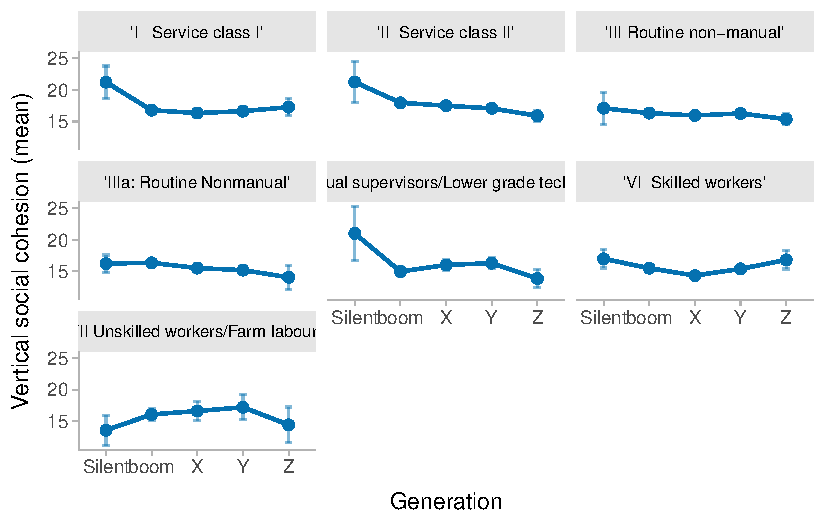
\includegraphics[keepaspectratio]{05-resultados_files/figure-pdf/fig-1-1.pdf}}

}

\end{figure}%

La figura presenta un análisis bivariado que examina la media de la
cohesión social vertical (eje Y) a través de cinco cohortes
generacionales (Generation: Silent, Boom, X, Y, Z, en el eje X),
segmentado o facetado por las distintas categorías del esquema de clase
social EGP-7. Las barras verticales alrededor de cada punto representan
los intervalos de confianza al 95\%, lo que permite evaluar la precisión
de las estimaciones y la significancia visual de las diferencias.

En primer lugar, se observa un efecto generacional parcialmente
consistente con la hipótesis H1, caracterizado por una tendencia
descendente de la cohesión social vertical a medida que las cohortes son
más jóvenes (de Silent hacia Z). Este patrón de ``caída'' generacional
es especialmente pronunciado y nítido en las clases socioeconómicas más
altas, como Service Class I y Service Class II, así como en las
ocupaciones de rutina no manuales (Routine non-manual y Routine
non-manual IIIa), donde los miembros de la generación Silent reportan
niveles de cohesión significativamente más altos (superando los 20
puntos en las clases de servicios) en comparación con las generaciones
sucesivas, las cuales tienden a estancarse o seguir descendiendo
sutilmente en torno a los 15-17 puntos.

En segundo lugar, el comportamiento de las clases manuales y
trabajadoras (EGP-V, VI y VII) quiebra la linealidad del descenso
generacional, mostrando dinámicas heterogéneas. En la categoría V
(Manual supervisors/Lower grade technicians) se aprecia un desplome
drástico entre la generación Silent y los Boomers, seguido de una leve
recuperación en las generaciones intermedias antes de volver a caer en
la generación Z. Por otro lado, la clase VI (Skilled workers) exhibe un
patrón en forma de ``U'': la cohesión disminuye desde la generación
Silent hasta alcanzar su punto más bajo en la Generación X, para luego
experimentar un repunte sistemático y estadísticamente visible en las
generaciones más jóvenes (Y y Z). Una tendencia inversa o de curva
invertida se observa en la clase VII (Unskilled workers/Farm labours),
donde la generación Silent inicia con los niveles de cohesión más bajos
(cercanos a 13 puntos), sube de forma sostenida hacia las generaciones
Boomer, X e Y, y vuelve a contraerse con la llegada de la generación Z.

\begin{figure}[H]

\caption{Gráficos del análisis Bivariado}

{\centering 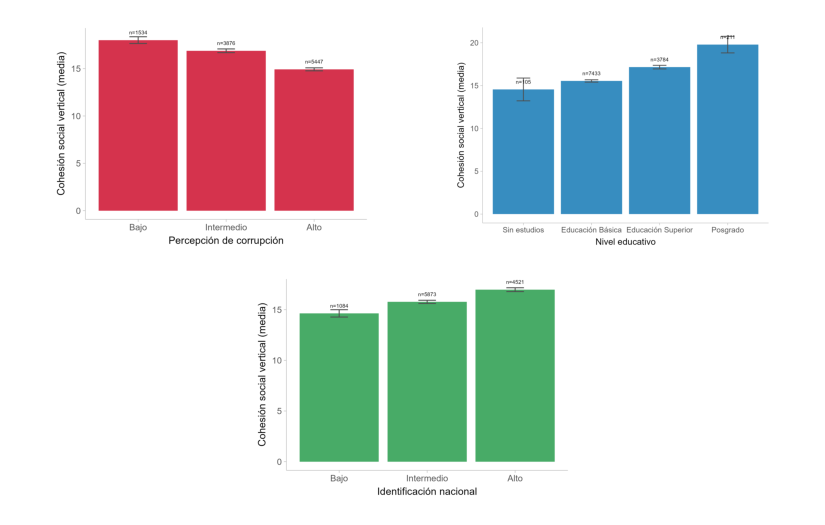
\includegraphics[width=1\linewidth,height=\textheight,keepaspectratio]{05-resultados_files/figure-pdf/bivariado2-1.pdf}

}

\end{figure}%

Aquellos individuos que perciben niveles bajos de corrupción reportan la
media más alta en el índice de cohesión social vertical, rozando los 18
puntos. Esta evaluación disminuye de manera progresiva a medida que la
percepción transita hacia niveles intermedios, alcanzando su punto más
deficiente en la categoría de alta corrupción, donde el indicador de
cohesión se contrae fuertemente hasta situarse justo en el límite de los
15 puntos.

En cuanto al nivel educativo, se observa una tendencia lineal
marcadamente ascendente que vincula el capital humano con la legitimidad
del sistema. Los niveles más bajos de cohesión social vertical se
concentran en el grupo de personas sin estudios, el cual se ubica por
debajo de los 15 puntos de media. A partir de ese umbral, la valoración
del lazo vertical experimenta un incremento constante y sucesivo al
pasar por la educación básica y la educación superior, alcanzando su
punto máximo e indiscutible en la población con estudios de posgrado,
cuya media se posiciona en la cúspide de la escala al rozar los 20
puntos.

Finalmente, el comportamiento de la identificación nacional devela una
relación directa y positiva con el orden institucional. Las personas que
manifiestan un sentido de identidad nacional bajo presentan un deterioro
evidente en su cohesión vertical, registrando puntuaciones por debajo de
los 15 puntos. En contraposición, a medida que el arraigo y el sentido
de pertenencia con el país se fortalecen hacia niveles intermedios y
altos, la media de la cohesión social vertical experimenta un aumento
sostenido, logrando superar con claridad la barrera de los 17 puntos en
la categoría más alta.

\begin{figure}[H]

\caption{Gráficos del análisis Bivariado}

{\centering 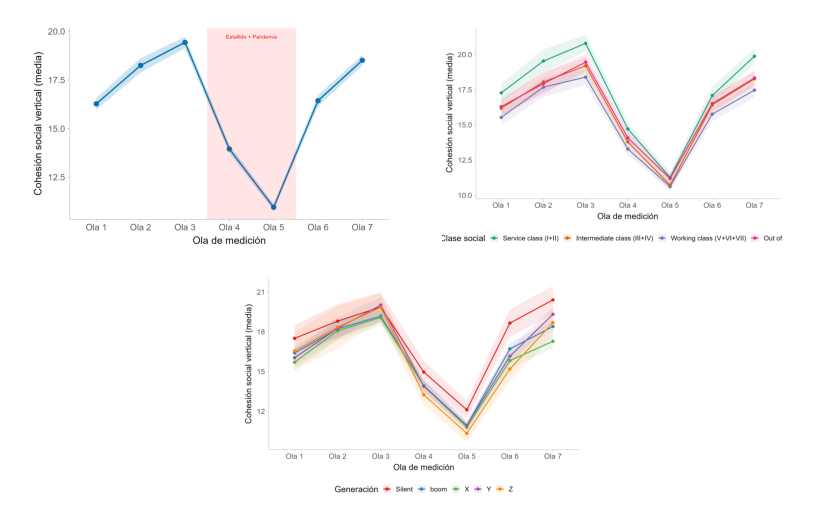
\includegraphics[width=1\linewidth,height=\textheight,keepaspectratio]{05-resultados_files/figure-pdf/bivariado3-1.pdf}

}

\end{figure}%

El análisis longitudinal revela una trayectoria temporal de la cohesión
social vertical altamente homogénea, marcada de forma dramática por el
contexto nacional. Se observa un aumento sostenido entre las Olas 1 y 3,
seguido de un quiebre abrupto en las Olas 4 y 5 que coincide exactamente
con el periodo del estallido social y la pandemia, donde el indicador
cae a su mínimo histórico. A partir de la Ola 6, el sistema muestra una
recuperación acelerada, retornando a los niveles iniciales hacia la Ola
7.

Al desagregar los datos, las brechas se mantienen estables en el tiempo,
sin que las crisis alteren el orden de los factores estructurales. Por
un lado, la clase de servicios y la generación Silent se posicionan de
manera persistente en la cúspide de la cohesión vertical, mientras que
la clase trabajadora permanece en la base. La única divergencia
relevante ocurre en la fase de recuperación post-pandemia (Olas 6 y 7),
donde las cohortes más jóvenes (Y y Z) exhiben un repunte o pendiente de
ascenso más pronunciado que la Generación X, sugiriendo una reactivación
diferenciada. \#\#\# Modelos de regresión multinivel.

{

\begin{longtable}[]{@{}lllllll@{}}

\caption{\label{tbl-modelos}Multilevel models for vertical social
cohesion}

\tabularnewline

\toprule\noalign{}
~ & Modelo 0 & Modelo Temp. & Modelo 1 & Modelo 2 & Modelo 3 & Modelo
4 \\
\midrule\noalign{}
\endhead
\midrule\noalign{}
\multicolumn{7}{@{}l@{}}{%
Note: Cells contain regression coefficients with standard errors in
parentheses. \textsuperscript{***}p \textless{} 0.001;
\textsuperscript{**}p \textless{} 0.01; \textsuperscript{*}p \textless{}
0.05.} \\
\bottomrule\noalign{}
\endlastfoot
Intercept & 15.848\textsuperscript{***} & 15.711\textsuperscript{***} &
17.915\textsuperscript{***} & 22.858\textsuperscript{***} &
23.195\textsuperscript{***} & 23.017\textsuperscript{***} \\
~ & (0.111) & (0.180) & (0.682) & (2.318) & (2.244) & (2.244) \\
Corruption perception (Specific-mean centered) & ~ & ~ &
-0.467\textsuperscript{***} & ~ & -0.480\textsuperscript{***} &
-0.494\textsuperscript{***} \\
~ & ~ & ~ & (0.090) & ~ & (0.075) & (0.077) \\
Corruption perception (Person historical mean) & ~ & ~ & ~ &
-2.113\textsuperscript{***} & -2.079\textsuperscript{***} &
-2.090\textsuperscript{***} \\
~ & ~ & ~ & ~ & (0.166) & (0.163) & (0.163) \\
Age (Specific-mean centered) & ~ & ~ & 0.072\textsuperscript{**} & ~ &
0.030 & -0.053 \\
~ & ~ & ~ & (0.028) & ~ & (0.045) & (0.078) \\
Age (Person historical mean) & ~ & ~ & ~ & 0.015 & 0.012 & 0.014 \\
~ & ~ & ~ & ~ & (0.023) & (0.022) & (0.022) \\
National identification (Specific-mean centered) & ~ & ~ &
0.674\textsuperscript{***} & ~ & 0.341\textsuperscript{***} &
0.340\textsuperscript{***} \\
~ & ~ & ~ & (0.100) & ~ & (0.083) & (0.083) \\
National identification (Person historical mean) & ~ & ~ & ~ &
1.221\textsuperscript{***} & 1.160\textsuperscript{***} &
1.162\textsuperscript{***} \\
~ & ~ & ~ & ~ & (0.200) & (0.195) & (0.195) \\
Dignified treatment (Specific-mean centered) & ~ & ~ &
0.167\textsuperscript{***} & ~ & -0.062\textsuperscript{**} &
-0.055\textsuperscript{**} \\
~ & ~ & ~ & (0.016) & ~ & (0.021) & (0.021) \\
Dignified treatment (Person historical mean) & ~ & ~ & ~ &
-0.309\textsuperscript{***} & -0.174\textsuperscript{***} &
-0.199\textsuperscript{***} \\
~ & ~ & ~ & ~ & (0.030) & (0.030) & (0.032) \\
Political self-identification (Specific-mean centered) & ~ & ~ & -0.035
& ~ & -0.111\textsuperscript{***} & -0.108\textsuperscript{***} \\
~ & ~ & ~ & (0.020) & ~ & (0.017) & (0.017) \\
Political self-identification (Person historical mean) & ~ & ~ & ~ &
-0.281\textsuperscript{***} & -0.293\textsuperscript{***} &
-0.297\textsuperscript{***} \\
~ & ~ & ~ & ~ & (0.039) & (0.038) & (0.038) \\
Sex: Female & ~ & ~ & ~ & -0.047 & -0.067 & -0.094 \\
~ & ~ & ~ & ~ & (0.200) & (0.195) & (0.196) \\
Education: Basic & ~ & ~ & ~ & 0.968 & 0.659 & 0.707 \\
~ & ~ & ~ & ~ & (0.997) & (0.873) & (0.861) \\
Education: Higher education & ~ & ~ & ~ & 2.221\textsuperscript{*} &
1.658 & 1.698 \\
~ & ~ & ~ & ~ & (1.013) & (0.888) & (0.876) \\
Education: Postgraduate & ~ & ~ & ~ & 3.782\textsuperscript{***} &
2.909\textsuperscript{**} & 2.969\textsuperscript{**} \\
~ & ~ & ~ & ~ & (1.142) & (1.001) & (0.991) \\
Generation: Boom & ~ & ~ & -1.893\textsuperscript{**} & -1.089 & -1.074
& -1.068 \\
~ & ~ & ~ & (0.705) & (0.699) & (0.689) & (0.688) \\
Generation: X & ~ & ~ & -2.323\textsuperscript{**} & -1.378 & -1.337 &
-1.327 \\
~ & ~ & ~ & (0.714) & (0.897) & (0.883) & (0.882) \\
Generation: Y & ~ & ~ & -2.012\textsuperscript{**} & -1.199 & -1.089 &
-1.052 \\
~ & ~ & ~ & (0.717) & (1.111) & (1.093) & (1.092) \\
Generation: Z & ~ & ~ & -2.661\textsuperscript{***} & -1.625 & -1.524 &
-1.481 \\
~ & ~ & ~ & (0.788) & (1.331) & (1.309) & (1.308) \\
Intermediate class (III+IV) & ~ & ~ & ~ & -0.585\textsuperscript{**} &
-0.419\textsuperscript{*} & -0.426\textsuperscript{*} \\
~ & ~ & ~ & ~ & (0.203) & (0.178) & (0.181) \\
Working class (V+VI+VII) & ~ & ~ & ~ & -0.930\textsuperscript{***} &
-0.812\textsuperscript{***} & -0.864\textsuperscript{***} \\
~ & ~ & ~ & ~ & (0.213) & (0.190) & (0.194) \\
Wave 2017 & ~ & 2.113\textsuperscript{***} & ~ & ~ &
1.409\textsuperscript{***} & 1.526\textsuperscript{***} \\
~ & ~ & (0.210) & ~ & ~ & (0.292) & (0.292) \\
Wave 2018 & ~ & 3.719\textsuperscript{***} & ~ & ~ &
3.463\textsuperscript{***} & 3.539\textsuperscript{***} \\
~ & ~ & (0.195) & ~ & ~ & (0.223) & (0.257) \\
Wave 2019 & ~ & -1.800\textsuperscript{***} & ~ & ~ &
-2.319\textsuperscript{***} & -2.090\textsuperscript{***} \\
~ & ~ & (0.194) & ~ & ~ & (0.307) & (0.367) \\
Wave 2021 & ~ & -4.866\textsuperscript{***} & ~ & ~ &
-5.585\textsuperscript{***} & -5.279\textsuperscript{***} \\
~ & ~ & (0.195) & ~ & ~ & (0.332) & (0.428) \\
Wave 2022 & ~ & 0.712\textsuperscript{***} & ~ & ~ & 0.053 & 0.516 \\
~ & ~ & (0.195) & ~ & ~ & (0.383) & (0.541) \\
Wave 2023 & ~ & 3.043\textsuperscript{***} & ~ & ~ &
2.242\textsuperscript{***} & 2.642\textsuperscript{***} \\
~ & ~ & (0.210) & ~ & ~ & (0.418) & (0.591) \\
BIC & 51120.934 & 48412.698 & 51007.369 & 50866.175 & 48179.382 &
48144.670 \\
Num. obs. & 7979 & 7979 & 7979 & 7979 & 7979 & 7979 \\
Num. groups: individuals & 1372 & 1372 & 1372 & 1372 & 1372 & 1372 \\
Var: individuals (Intercept) & 11.697 & 12.197 & 11.668 & 7.386 & 8.650
& 8.804 \\
Var: individuals (Age within) & 28.789 & 19.238 & 27.953 & 28.811 &
18.991 & 17.772 \\
Cov: individuals (Intercept - Age within) & ~ & ~ & ~ & ~ & ~ & 0.195 \\
Var: Residual & ~ & ~ & ~ & ~ & ~ & -0.091 \\

\end{longtable}

}

El análisis de los determinantes de la confianza en las instituciones se
abordó mediante una estrategia de modelación de efectos mixtos, idónea
para capturar de manera simultánea la variabilidad entre individuos y
los cambios a lo largo del tiempo durante el periodo 2016-2023.
Siguiendo las recomendaciones metodológicas de Enders y Tofighi (2007),
se procedió al centrado a la media de grupo (CWC) para las variables de
Nivel 1 y a la inclusión de los promedios históricos en el Nivel 2. Esta
especificación es fundamental para la correcta interpretación de los
hallazgos, puesto que la estimación de los coeficientes de Nivel 1
permite aislar el efecto within (intra-individual) puro, garantizando
que las fluctuaciones anuales específicas estén controladas por el
promedio histórico del sujeto. Por su parte, el coeficiente de la
variable grupal en el Nivel 2 representa el efecto between
(inter-individual), permitiendo una diferenciación teórica y empírica
nítida entre dinámicas longitudinales e individuales. Como paso
analítico previo, el Modelo 0 (Nulo) permitió realizar la partición de
la varianza y calcular la Correlación Intraclase (ICC) con el fin de
evaluar la pertinencia del anidamiento de los datos. A partir de una
varianza de intercepto (\(\tau_{00}\)) de 11.697 y una varianza residual
(\(\sigma^2\)) de 28.789, se obtuvo un ICC de aproximadamente 0.289.
Este resultado indica que el 28.9\% de la varianza en la confianza
institucional se explica por diferencias estables y estructurales entre
las personas, mientras que el 71.1\% restante responde a fluctuaciones
temporales endógenas o a errores de medición. Al superar ampliamente el
umbral crítico del 10\%, este indicador justifica técnicamente el empleo
de modelos multinivel, evitando así sesgos potenciales en las
inferencias estadísticas subsiguientes. Al examinar los predictores
sustantivos en el Modelo 4 (modelo final), la percepción de corrupción
manifiesta ser el detractor más robusto y severo de la confianza
institucional. Bajo la lógica de Enders y Tofighi, se evidencia un
marcado contraste entre el efecto crónico y el shock puntual: el
promedio histórico de la percepción de corrupción de un individuo
(efecto between) ejerce un impacto devastador (\(\beta = -2.090\),
\(p < 0.001\)) que cuadruplica la magnitud de una fluctuación anual
específica (efecto within, \(\beta = -0.494\), \(p < 0.001\)). Esto
sugiere de forma contundente que la confianza no se erosiona de manera
irreversible por escándalos aislados, sino por una evaluación sistémica
y prolongada de falta de integridad en el entorno, coincidiendo con el
diagnóstico de la OCDE sobre la prioridad de la integridad pública para
reconstruir el vínculo ciudadano. En una dirección opuesta, la
identificación nacional se ratifica como el principal motor de
resiliencia y cohesión social; en consonancia con los planteamientos de
Schiefer (2016), su promedio histórico presenta un fuerte efecto
positivo (\(\beta = 1.162\), \(p < 0.001\)), actuando como un potente
amortiguador cultural. Por otro lado, el comportamiento de las variables
de estratificación y capital humano manifiesta importantes fracturas de
carácter estructural y generacional. Un hallazgo metodológico y teórico
fundamental ocurre al observar la transición entre los modelos: en el
Modelo Temporal, las variables de generación (Boomers, X e Y) mostraban
efectos negativos significativos; sin embargo, al controlar por el
promedio histórico de la variable individual edad (Nivel 2) a partir del
Modelo 1, el efecto de estas variables generacionales pierde su
significancia estadística. Esto demuestra que la aparente desconfianza
atribuida a la cohorte era absorbida por el efecto puramente biográfico
y longitudinal de la edad acumulada. La única excepción a esta regla es
la Generación Z, la cual mantiene un distanciamiento estructural,
robusto y estadísticamente significativo frente a las instituciones
publicas (\(\beta = -1.481\)), sugiriendo que los jóvenes más australes
han abandonado los surcos de legitimación tradicional en favor de
perfiles más críticos e independientes.En cuanto a la estructura de
clases, los resultados exponen una brecha socioeconómica evidente: tanto
la clase intermedia (\(\beta = -0.426\), \(p < 0.05\)) como la clase
trabajadora manual (\(\beta = -0.864\), \(p < 0.001\)) exhiben niveles
de confianza significativamente menores en comparación con la clase de
servicios de referencia, validando el diagnóstico de Molina y Alfageme
(2022) sobre la exclusión material y subjetiva del pacto social en
América Latina. Finalmente, respecto al capital educativo se observa una
tendencia monótonamente creciente en los coeficientes, aunque únicamente
el nivel de Posgrado se consolida como un habilitador estadísticamente
significativo (\(\beta = 2.969\), \(p < 0.01\)). Cabe destacar que el
modelo final constató la estabilidad de estas brechas estructurales a
través del tiempo, dado que la varianza y covarianza de las pendientes
aleatorias resultaron marginales.Finalmente, la dimensión temporal del
modelo captura con precisión la trayectoria histórica reciente del
contexto chileno a través de los coeficientes asignados a las olas de
medición en comparación con la Ola basal de 2016. Tras repuntes
significativos en 2017 (\(\beta = 1.526\), \(p < 0.001\)) y 2018
(\(\beta = 3.539\), \(p < 0.001\)), se registra una caída estrepitosa
del indicador de confianza hacia la Ola 2019 (\(\beta = -2.090\),
\(p < 0.001\)) y especialmente en la Ola 2021 (\(\beta = -5.279\),
\(p < 0.001\)), reflejando el impacto acumulado y erosivo del estallido
social y la subsiguiente crisis de la pandemia. No obstante, al avanzar
hacia la Ola 2023, los datos muestran un fuerte repunte estadísticamente
significativo (\(\beta = 2.642\), \(p < 0.001\)), sugiriendo una fase de
estabilización institucional tras el periodo de mayor agitación. En
contraste con estos movimientos, la variable de Trato Digno arrojó un
comportamiento contraintuitivo respecto a las expectativas teóricas,
registrando coeficientes negativos tanto en su componente within
(\(\beta = -0.055\), \(p < 0.01\)) como between (\(\beta = -0.199\),
\(p < 0.001\)) en el modelo final, lo que plantea la necesidad de
revisar su operacionalización en escenarios de alta desafección
ciudadana.

Cabe mencionar que el \(R^2\) marginal de el último modelo reportado fue
de 0.293 lo que indica que los predictores fijos del estudio explican
por sí solos casi un tercio de la variabilidad en la confianza
institucional. \(R^2\) condicional, por su parte, que integra efectos
fijos y aleatorios fue de 54.3\%. Esta diferencia confirma que una parte
sustancial de la desconfianza en Chile es un rasgo crónico y persistente
de los individuos que trasciende las fluctuaciones anuales.

\bookmarksetup{startatroot}

\chapter{Conclusiones}\label{conclusiones}

A partir de los resultados obtenidos mediante la modelación de regresión
multinivel y su posterior contraste con la literatura teórica y
empírica, es posible establecer conclusiones fundamentales sobre la
dinámica de la confianza institucional en Chile durante el periodo
2016-2023. El hallazgo más contundente de esta investigación determina
que la percepción de corrupción constituye el principal detractor de la
confianza en las instituciones públicas. Al adoptar la desagregación
metodológica de Enders \& Tofighi
(\citeproc{ref-enders_centering_2007}{2007}), se constata que el
promedio histórico de un individuo (efecto \emph{between}) posee un
impacto adverso cuatro veces superior al de las fluctuaciones anuales
puntuales (efecto \emph{within}). Este resultado valida los diagnósticos
de la {«{La confianza en las instituciones públicas de Chile}»}
(\citeproc{ref-_confianza_2024}{2024}), que posicionan a la integridad
pública como el pilar analítico del contrato social. No obstante, la
evidencia empírica aporta un matiz crítico, ya que la confianza
institucional en Chile no se erosiona coyunturalmente por escándalos
aislados o de corto plazo, sino por una evaluación sistémica, acumulada
y cronificada de la probidad en el tiempo. Se corrobora así que la
integridad no es un simple resultado del desempeño, sino una
precondición estructural para la legitimidad del sistema político, tal
como postulan {«({PDF}) {The Essentials} of {Social Cohesion}»}
(\citeproc{ref-_essentials_2017}{2017}).

En contraposición a la volatilidad que caracteriza a la confianza
institucional, el sentido de pertenencia e identificación con el país se
consolida como el predictor de resiliencia más robusto dentro del modelo
estadístico. Este fenómeno se alinea con la tesis de {«({PDF}) {The
Essentials} of {Social Cohesion}»}
(\citeproc{ref-_essentials_2017}{2017}), quien define la identificación
colectiva como una dimensión constitutiva y esencial de la cohesión
social, diferenciándose de aquellas variables supeditadas al rendimiento
instrumental del Estado. En el escenario chileno, la identidad nacional
opera como una reserva cultural o amortiguador axiológico que sostiene
el vínculo entre la sociedad y el Estado, incluso ante crisis severas de
legitimidad representativa. Surge aquí una divergencia respecto a las
advertencias de la {«{La confianza en las instituciones públicas de
Chile}»} (\citeproc{ref-_confianza_2024}{2024}) sobre cómo la
desigualdad fractura el destino compartido, puesto que los datos
demuestran que este arraigo subjetivo permanece como el ancla más
estable del sistema a pesar de las profundas brechas socioeconómicas que
caracterizan al país.

Por otra parte, los modelos estimados exponen que la confianza
institucional se distribuye de manera asimétrica en la estructura
social, revelando quiebres estructurales que desafían ciertas premisas
de la literatura internacional. En primer lugar, la clase trabajadora
manual presenta los niveles de confianza más bajos del panel, lo cual
contradice parcialmente las tesis globales de Kim et~al.
(\citeproc{ref-kim_social_2021}{2021}), quienes sugieren que las clases
altas tienden a ser más críticas debido a estándares de evaluación
técnica más exigentes. Para el caso chileno, se constata más bien la
vigencia de la hipótesis de heterogeneidad estructural descrita por
Molina \& Alfageme (\citeproc{ref-molina_repensando_2022}{2022}), donde
la exclusión material en el mercado laboral se traduce directamente en
una desafección del pacto social. En segundo lugar, se identifica una
excepcionalidad en la Generación Z; mientras que el escepticismo en
otras cohortes tiende a ser absorbido por el efecto del envejecimiento
biográfico, esta generación manifiesta un distanciamiento estructural
significativo. Este hallazgo sintoniza con el perfil de los sectores
movilizados propuesto por \emph{{Cohesión social en Chile en tiempos de
cambio}} (\citeproc{ref-_cohesion_2022}{2022}), caracterizado por
cohortes juveniles con alta disposición a la participación horizontal
pero con una nula validación de las jerarquías tradicionales, hoy en día
confirmando una salida sistemática del surco de legitimidad tradicional.

Asimismo, el análisis longitudinal logra capturar con precisión la
sensibilidad del indicador frente a los hitos históricos recientes del
país, mostrando una contracción severa en la medición de 2021 que
refleja el impacto erosivo acumulado y sinérgico del estallido social de
2019 y la crisis sanitaria por COVID-19. Este comportamiento convalida
la perspectiva de la \emph{{Cohesión social en Chile en tiempos de
cambio}} (\citeproc{ref-_cohesion_2022}{2022}) respecto a la fragilidad
de la cohesión social vertical en escenarios de alta incertidumbre. Sin
embargo, el repunte estadísticamente significativo identificado en la
ola de 2023 introduce un matiz de estabilización que la literatura
reactiva del año 2020 no logró prever, sugiriendo una capacidad de
recuperación parcial y un retorno hacia una meseta de equilibrio tras el
periodo de mayor agitación civil.

Finalmente, la investigación revela un resultado imprevisto y de alta
relevancia teórica respecto al comportamiento de la variable asociada al
trato digno, la cual reportó coeficientes negativos tanto en su
dimensión temporal como en su componente transversal. Este matiz crítico
contradice la expectativa formulada por el Ministerio de Desarrollo
Social y Familia
(\citeproc{ref-ministeriodedesarrollosocialyfamilia_informe_2020}{2020}),
que proyectaba al trato digno como el principal articulador micro-social
de las interacciones cotidianas. La evidencia sugiere que, en contextos
de profunda desafección ciudadana, la demanda por dignidad adquiere un
carácter maximalista. Por consiguiente, mejoras marginales o
superficiales en los niveles de trato pueden ser percibidas por los
individuos como insuficientes o cínicas, un hallazgo que releva la
necesidad de revisar urgentemente la operacionalización de este
constructo al ser evaluado en sociedades con fracturas estructurales
complejas.

\bookmarksetup{startatroot}

\chapter{Referencias}\label{referencias}

\cleardoublepage
\phantomsection
\addcontentsline{toc}{part}{Apéndices}
\appendix

\chapter{Preparación de Datos}\label{preparaciuxf3n-de-datos}

Cohesión Social Vertical en Chile (2016--2023)

\hfill\break

\chapter{Presentación}\label{presentaciuxf3n}

Este documento detalla el proceso de preparación de datos para el
análisis de la cohesión social vertical en Chile entre 2016 y 2023,
utilizando los datos del Estudio Longitudinal Social de Chile (ELSOC).
Se describen y justifican todas las decisiones de procesamiento, desde
la limpieza inicial hasta la construcción de variables analíticas y el
centrado para modelos multinivel.

\chapter{Librerías}\label{libreruxedas}

\begin{Shaded}
\begin{Highlighting}[]
\FunctionTok{library}\NormalTok{(haven)}
\FunctionTok{library}\NormalTok{(dplyr)}
\FunctionTok{library}\NormalTok{(tidyr)}
\FunctionTok{library}\NormalTok{(lme4)}
\FunctionTok{library}\NormalTok{(DIGCLASS)}
\FunctionTok{library}\NormalTok{(stringr)}
\FunctionTok{options}\NormalTok{(}\AttributeTok{scipen =} \DecValTok{999}\NormalTok{)}
\FunctionTok{rm}\NormalTok{(}\AttributeTok{list =} \FunctionTok{ls}\NormalTok{())}
\FunctionTok{library}\NormalTok{(here)}
\end{Highlighting}
\end{Shaded}

\chapter{Lectura y limpieza inicial}\label{lectura-y-limpieza-inicial}

\section{Lectura de datos}\label{lectura-de-datos}

Los datos provienen de ELSOC en su versión longitudinal 2016--2023, en
formato Stata (\texttt{.dta}).

\begin{Shaded}
\begin{Highlighting}[]
\NormalTok{elsoc }\OtherTok{\textless{}{-}} \FunctionTok{readRDS}\NormalTok{(}\FunctionTok{here}\NormalTok{(}\StringTok{"input"}\NormalTok{, }\StringTok{"ELSOC\_variables\_estudio.rds"}\NormalTok{))}
\FunctionTok{colnames}\NormalTok{(elsoc)}
\end{Highlighting}
\end{Shaded}

\begin{verbatim}
 [1] "idencuesta"    "ola"           "tipo_atricion" "c05_01"       
 [5] "c05_02"        "c05_03"        "c05_04"        "c05_05"       
 [9] "c05_06"        "c05_07"        "c05_08"        "c05_09"       
[13] "c35_01"        "c35_02"        "c35_03"        "c38"          
[17] "c32_01"        "c15"           "m53"           "m0_edad"      
[21] "m0_sexo"       "m01"           "ciuo88_m03"    "ciuo08_m03"   
[25] "m02"           "m07"           "m06"          
\end{verbatim}

\section{Limpieza de códigos perdidos y filtro de
muestra}\label{limpieza-de-cuxf3digos-perdidos-y-filtro-de-muestra}

ELSOC codifica los valores perdidos con códigos numéricos especiales
(−999, −888, −777, −666), que corresponden a distintas razones de no
respuesta (rechazo, no sabe, error técnico, encuesta incompleta). Estos
códigos se reemplazan por \texttt{NA} para todas las variables numéricas
y de carácter.

Adicionalmente, se restringe la muestra a los respondentes con
\texttt{tipo\_atricion\ ==\ 1}, que corresponde a quienes participaron
de forma continua en el panel. Esta decisión asegura que los modelos
longitudinales se estimen sobre trayectorias completas y comparables
entre individuos.

\begin{Shaded}
\begin{Highlighting}[]
\NormalTok{data }\OtherTok{\textless{}{-}}\NormalTok{ elsoc }\SpecialCharTok{\%\textgreater{}\%}
  \FunctionTok{mutate}\NormalTok{(}
    \FunctionTok{across}\NormalTok{(}
      \FunctionTok{where}\NormalTok{(is.numeric),}
      \SpecialCharTok{\textasciitilde{}} \FunctionTok{na\_if}\NormalTok{(}\FunctionTok{na\_if}\NormalTok{(}\FunctionTok{na\_if}\NormalTok{(}\FunctionTok{na\_if}\NormalTok{(.x, }\SpecialCharTok{{-}}\DecValTok{999}\NormalTok{), }\SpecialCharTok{{-}}\DecValTok{888}\NormalTok{), }\SpecialCharTok{{-}}\DecValTok{777}\NormalTok{), }\SpecialCharTok{{-}}\DecValTok{666}\NormalTok{)}
\NormalTok{    ),}
    \FunctionTok{across}\NormalTok{(}
      \FunctionTok{where}\NormalTok{(is.character) }\SpecialCharTok{|} \FunctionTok{where}\NormalTok{(is.factor),}
      \SpecialCharTok{\textasciitilde{}} \FunctionTok{na\_if}\NormalTok{(}\FunctionTok{na\_if}\NormalTok{(}\FunctionTok{na\_if}\NormalTok{(}\FunctionTok{na\_if}\NormalTok{(}\FunctionTok{as.character}\NormalTok{(.x), }\StringTok{"{-}999"}\NormalTok{), }\StringTok{"{-}888"}\NormalTok{), }\StringTok{"{-}777"}\NormalTok{), }\StringTok{"{-}666"}\NormalTok{)}
\NormalTok{    )}
\NormalTok{  ) }\SpecialCharTok{\%\textgreater{}\%}
\NormalTok{  \{}
    \ControlFlowTok{if}\NormalTok{ (}\StringTok{"tipo\_atricion"} \SpecialCharTok{\%in\%} \FunctionTok{names}\NormalTok{(.)) \{}
\NormalTok{      dplyr}\SpecialCharTok{::}\FunctionTok{filter}\NormalTok{(., .data[[}\StringTok{"tipo\_atricion"}\NormalTok{]] }\SpecialCharTok{==} \DecValTok{1}\NormalTok{)}
\NormalTok{    \} }\ControlFlowTok{else}\NormalTok{ \{}
\NormalTok{      .}
\NormalTok{    \}}
\NormalTok{  \}}
\end{Highlighting}
\end{Shaded}

\chapter{Construcción de variables
base}\label{construcciuxf3n-de-variables-base}

\section{Ola, trato digno e identificación
indígena}\label{ola-trato-digno-e-identificaciuxf3n-induxedgena}

La variable \texttt{ola} se convierte en factor etiquetado. La
percepción de meritocracia (\texttt{c32\_01}) se trata como variable
ordinal de cinco categorías (\texttt{c32\_01\_ord}). La pertenencia a
pueblo indígena (\texttt{indigena}) se construye como variable
dicotómica a partir del ítem \texttt{m53}, que registra la
autoidentificación con algún pueblo originario.

Los índices de participación organizacional (\texttt{c05\_total}) y
trato digno (\texttt{trato\_digno}) se construyen como sumas aditivas de
sus ítems componentes. Para el indicador de trato digno, los valores
ausentes (NA) se imputaron mediante arrastre hacia adelante (forward
fill) a nivel de individuo, reemplazando el vacío de una ola únicamente
si existía un valor válido en la medición inmediatamente anterior.

\begin{Shaded}
\begin{Highlighting}[]
\CommentTok{\# 1. Creamos las variables base y aplicamos las condiciones sobre \textquotesingle{}data\textquotesingle{}}
\NormalTok{data }\OtherTok{\textless{}{-}}\NormalTok{ data }\SpecialCharTok{\%\textgreater{}\%}
  \FunctionTok{mutate}\NormalTok{(}
    \AttributeTok{ola =} \FunctionTok{factor}\NormalTok{(ola, }\AttributeTok{levels =} \DecValTok{1}\SpecialCharTok{:}\DecValTok{7}\NormalTok{, }\AttributeTok{labels =} \FunctionTok{paste0}\NormalTok{(}\StringTok{"Ola "}\NormalTok{, }\DecValTok{1}\SpecialCharTok{:}\DecValTok{7}\NormalTok{)),}
    \AttributeTok{c32\_01 =}\NormalTok{ readr}\SpecialCharTok{::}\FunctionTok{parse\_number}\NormalTok{(}\FunctionTok{as.character}\NormalTok{(c32\_01)),}
    \AttributeTok{c32\_01\_ord =} \FunctionTok{factor}\NormalTok{(c32\_01, }\AttributeTok{levels =} \DecValTok{1}\SpecialCharTok{:}\DecValTok{5}\NormalTok{, }\AttributeTok{ordered =} \ConstantTok{TRUE}\NormalTok{),}
    \AttributeTok{m53\_label =}\NormalTok{ haven}\SpecialCharTok{::}\FunctionTok{as\_factor}\NormalTok{(m53, }\AttributeTok{levels =} \StringTok{"labels"}\NormalTok{),}
    \AttributeTok{indigena =} \FunctionTok{case\_when}\NormalTok{(}
\NormalTok{      m53\_label }\SpecialCharTok{==} \StringTok{"Ninguno"} \SpecialCharTok{\textasciitilde{}} \DecValTok{0}\NormalTok{,}
\NormalTok{      m53\_label }\SpecialCharTok{\%in\%} \FunctionTok{c}\NormalTok{(}
        \StringTok{"Otro"}\NormalTok{, }\StringTok{"Yagan o Yamana"}\NormalTok{, }\StringTok{"Kawesqar"}\NormalTok{, }\StringTok{"Diaguita"}\NormalTok{, }\StringTok{"Colla"}\NormalTok{,}
        \StringTok{"Quechua"}\NormalTok{, }\StringTok{"Likan Antai"}\NormalTok{, }\StringTok{"Linkan Antai"}\NormalTok{, }\StringTok{"Rapa Nui"}\NormalTok{,}
        \StringTok{"Aimara"}\NormalTok{, }\StringTok{"Mapuche"}
\NormalTok{      ) }\SpecialCharTok{\textasciitilde{}} \DecValTok{1}\NormalTok{,}
\NormalTok{      m53\_label }\SpecialCharTok{\%in\%} \FunctionTok{c}\NormalTok{(}
        \StringTok{"No Responde"}\NormalTok{, }\StringTok{"No Sabe"}\NormalTok{,}
        \StringTok{"Valor perdido por error tecnico"}\NormalTok{,}
        \StringTok{"Valor perdido por encuesta incompleta"}
\NormalTok{      ) }\SpecialCharTok{\textasciitilde{}} \ConstantTok{NA\_real\_}\NormalTok{,}
      \ConstantTok{TRUE} \SpecialCharTok{\textasciitilde{}} \ConstantTok{NA\_real\_}
\NormalTok{    ),}
    \AttributeTok{c05\_total =} \FunctionTok{rowSums}\NormalTok{(}\FunctionTok{pick}\NormalTok{(c05\_01}\SpecialCharTok{:}\NormalTok{c05\_09), }\AttributeTok{na.rm =} \ConstantTok{TRUE}\NormalTok{),}
    \AttributeTok{trato\_digno =} \FunctionTok{rowSums}\NormalTok{(}\FunctionTok{pick}\NormalTok{(c35\_01}\SpecialCharTok{:}\NormalTok{c35\_03), }\AttributeTok{na.rm =} \ConstantTok{TRUE}\NormalTok{)}
\NormalTok{  ) }\SpecialCharTok{\%\textgreater{}\%}
  
  \CommentTok{\# 2. Forward Fill aplicado únicamente a \textquotesingle{}trato\_digno\textquotesingle{} a nivel de individuo}
  \FunctionTok{arrange}\NormalTok{(idencuesta, ola) }\SpecialCharTok{\%\textgreater{}\%} 
  \FunctionTok{group\_by}\NormalTok{(idencuesta) }\SpecialCharTok{\%\textgreater{}\%} 
\NormalTok{  tidyr}\SpecialCharTok{::}\FunctionTok{fill}\NormalTok{(trato\_digno, }\AttributeTok{.direction =} \StringTok{"down"}\NormalTok{) }\SpecialCharTok{\%\textgreater{}\%} 
  \FunctionTok{ungroup}\NormalTok{()}
\end{Highlighting}
\end{Shaded}

\section{Imputación de identificación
indígena}\label{imputaciuxf3n-de-identificaciuxf3n-induxedgena}

La variable \texttt{indigena} solo fue medida sistemáticamente en Ola 3.
Dado que la autoidentificación étnica es un atributo estable en el
tiempo ---es poco probable que una persona cambie su percepción sobre si
pertenece o no a un pueblo originario--- se imputa el valor de Ola 3
hacia todas las demás olas del mismo individuo.

\begin{Shaded}
\begin{Highlighting}[]
\NormalTok{data }\OtherTok{\textless{}{-}}\NormalTok{ data }\SpecialCharTok{\%\textgreater{}\%}
  \FunctionTok{group\_by}\NormalTok{(idencuesta) }\SpecialCharTok{\%\textgreater{}\%}
  \FunctionTok{mutate}\NormalTok{(}
    \AttributeTok{indigena\_ola3 =} \ControlFlowTok{if}\NormalTok{ (}\FunctionTok{any}\NormalTok{(ola }\SpecialCharTok{==} \StringTok{"Ola 3"} \SpecialCharTok{\&} \SpecialCharTok{!}\FunctionTok{is.na}\NormalTok{(indigena)))}
\NormalTok{      indigena[}\FunctionTok{which}\NormalTok{(ola }\SpecialCharTok{==} \StringTok{"Ola 3"} \SpecialCharTok{\&} \SpecialCharTok{!}\FunctionTok{is.na}\NormalTok{(indigena))[}\DecValTok{1}\NormalTok{]]}
    \ControlFlowTok{else} \ConstantTok{NA\_real\_}
\NormalTok{  ) }\SpecialCharTok{\%\textgreater{}\%}
  \FunctionTok{ungroup}\NormalTok{() }\SpecialCharTok{\%\textgreater{}\%}
  \FunctionTok{mutate}\NormalTok{(}\AttributeTok{indigena =} \FunctionTok{coalesce}\NormalTok{(indigena, indigena\_ola3)) }\SpecialCharTok{\%\textgreater{}\%}
  \FunctionTok{select}\NormalTok{(}\SpecialCharTok{{-}}\NormalTok{indigena\_ola3)}
\end{Highlighting}
\end{Shaded}

\chapter{Variables temporales y cohortes
generacionales}\label{variables-temporales-y-cohortes-generacionales}

La generación de pertenencia se deriva del año de nacimiento estimado,
calculado restando la edad máxima registrada en el panel al año 2023.
Este procedimiento asigna a cada individuo un año de nacimiento fijo,
independiente de la ola, y lo clasifica en una de cinco cohortes
generacionales.

\begin{Shaded}
\begin{Highlighting}[]
\NormalTok{safe\_max }\OtherTok{\textless{}{-}} \ControlFlowTok{function}\NormalTok{(x) \{}
\NormalTok{  x }\OtherTok{\textless{}{-}}\NormalTok{ x[}\SpecialCharTok{!}\FunctionTok{is.na}\NormalTok{(x)]}
  \ControlFlowTok{if}\NormalTok{ (}\FunctionTok{length}\NormalTok{(x) }\SpecialCharTok{==} \DecValTok{0}\NormalTok{) }\ConstantTok{NA\_real\_} \ControlFlowTok{else} \FunctionTok{max}\NormalTok{(x)}
\NormalTok{\}}

\NormalTok{data }\OtherTok{\textless{}{-}}\NormalTok{ data }\SpecialCharTok{\%\textgreater{}\%}
  \FunctionTok{group\_by}\NormalTok{(idencuesta) }\SpecialCharTok{\%\textgreater{}\%}
  \FunctionTok{mutate}\NormalTok{(}
    \AttributeTok{edad\_2023 =} \FunctionTok{safe\_max}\NormalTok{(m0\_edad),}
    \AttributeTok{anio\_nac =} \DecValTok{2023} \SpecialCharTok{{-}}\NormalTok{ edad\_2023,}
    \AttributeTok{Generacion =} \FunctionTok{case\_when}\NormalTok{(}
      \FunctionTok{between}\NormalTok{(anio\_nac, }\DecValTok{1930}\NormalTok{, }\DecValTok{1948}\NormalTok{) }\SpecialCharTok{\textasciitilde{}} \StringTok{"Silent"}\NormalTok{,}
      \FunctionTok{between}\NormalTok{(anio\_nac, }\DecValTok{1949}\NormalTok{, }\DecValTok{1968}\NormalTok{) }\SpecialCharTok{\textasciitilde{}} \StringTok{"boom"}\NormalTok{,}
      \FunctionTok{between}\NormalTok{(anio\_nac, }\DecValTok{1969}\NormalTok{, }\DecValTok{1980}\NormalTok{) }\SpecialCharTok{\textasciitilde{}} \StringTok{"X"}\NormalTok{,}
      \FunctionTok{between}\NormalTok{(anio\_nac, }\DecValTok{1981}\NormalTok{, }\DecValTok{1993}\NormalTok{) }\SpecialCharTok{\textasciitilde{}} \StringTok{"Y"}\NormalTok{,}
      \FunctionTok{between}\NormalTok{(anio\_nac, }\DecValTok{1994}\NormalTok{, }\DecValTok{2010}\NormalTok{) }\SpecialCharTok{\textasciitilde{}} \StringTok{"Z"}\NormalTok{,}
      \ConstantTok{TRUE} \SpecialCharTok{\textasciitilde{}} \ConstantTok{NA\_character\_}
\NormalTok{    ),}
    \AttributeTok{Generacion =} \FunctionTok{factor}\NormalTok{(Generacion, }\AttributeTok{levels =} \FunctionTok{c}\NormalTok{(}\StringTok{"Silent"}\NormalTok{, }\StringTok{"boom"}\NormalTok{, }\StringTok{"X"}\NormalTok{, }\StringTok{"Y"}\NormalTok{, }\StringTok{"Z"}\NormalTok{))}
\NormalTok{  ) }\SpecialCharTok{\%\textgreater{}\%}
  \FunctionTok{ungroup}\NormalTok{()}
\end{Highlighting}
\end{Shaded}

\chapter{Construcción de clase
social}\label{construcciuxf3n-de-clase-social}

\section{Esquema EGP-7}\label{esquema-egp-7}

La clase social se construye siguiendo el esquema EGP
(\emph{Erikson-Goldthorpe-Portocarrero}) de siete clases mediante el
paquete \texttt{DIGCLASS}. Este esquema requiere tres insumos: el código
ocupacional en ISCO-88, la situación de empleo y el número de
subordinados.

Los códigos ocupacionales disponibles en ISCO-08 (Olas 3, 5 y 7) se
convierten a ISCO-88. Dado que la ocupación no se midió en todas las
olas, los códigos ocupacionales y las variables auxiliares de empleo se
propagan hacia adelante y hacia atrás dentro de cada individuo
(\emph{fill down-up}), bajo el supuesto de que la posición ocupacional
es relativamente estable en el tiempo.

\begin{Shaded}
\begin{Highlighting}[]
\ControlFlowTok{if}\NormalTok{ (}\FunctionTok{requireNamespace}\NormalTok{(}\StringTok{"DIGCLASS"}\NormalTok{, }\AttributeTok{quietly =} \ConstantTok{TRUE}\NormalTok{)) \{}

\NormalTok{  data }\OtherTok{\textless{}{-}}\NormalTok{ data }\SpecialCharTok{\%\textgreater{}\%}
    \FunctionTok{arrange}\NormalTok{(idencuesta, ola) }\SpecialCharTok{\%\textgreater{}\%}
    \FunctionTok{mutate}\NormalTok{(}
      \AttributeTok{isco88\_raw =} \FunctionTok{case\_when}\NormalTok{(}
\NormalTok{        ola }\SpecialCharTok{==} \StringTok{"Ola 1"} \SpecialCharTok{\textasciitilde{}} \FunctionTok{formatC}\NormalTok{(}\FunctionTok{suppressWarnings}\NormalTok{(}\FunctionTok{as.integer}\NormalTok{(ciuo88\_m03)), }\AttributeTok{width =} \DecValTok{4}\NormalTok{, }\AttributeTok{flag =} \StringTok{"0"}\NormalTok{),}
        \ConstantTok{TRUE} \SpecialCharTok{\textasciitilde{}} \ConstantTok{NA\_character\_}
\NormalTok{      ),}
      \AttributeTok{isco88\_raw =} \FunctionTok{na\_if}\NormalTok{(isco88\_raw, }\StringTok{"  NA"}\NormalTok{),}
      \AttributeTok{ciuo08\_clean =} \FunctionTok{case\_when}\NormalTok{(}
\NormalTok{        ola }\SpecialCharTok{\%in\%} \FunctionTok{c}\NormalTok{(}\StringTok{"Ola 3"}\NormalTok{, }\StringTok{"Ola 5"}\NormalTok{, }\StringTok{"Ola 7"}\NormalTok{) }\SpecialCharTok{\textasciitilde{}} \FunctionTok{formatC}\NormalTok{(}\FunctionTok{suppressWarnings}\NormalTok{(readr}\SpecialCharTok{::}\FunctionTok{parse\_number}\NormalTok{(}\FunctionTok{as.character}\NormalTok{(ciuo08\_m03))), }\AttributeTok{width =} \DecValTok{4}\NormalTok{, }\AttributeTok{flag =} \StringTok{"0"}\NormalTok{),}
        \ConstantTok{TRUE} \SpecialCharTok{\textasciitilde{}} \ConstantTok{NA\_character\_}
\NormalTok{      ),}
      \AttributeTok{ciuo08\_clean =} \FunctionTok{na\_if}\NormalTok{(ciuo08\_clean, }\StringTok{"  NA"}\NormalTok{)}
\NormalTok{    )}

\NormalTok{  data}\SpecialCharTok{$}\NormalTok{isco88\_from08 }\OtherTok{\textless{}{-}} \ConstantTok{NA\_character\_}
\NormalTok{  idx08 }\OtherTok{\textless{}{-}} \SpecialCharTok{!}\FunctionTok{is.na}\NormalTok{(data}\SpecialCharTok{$}\NormalTok{ciuo08\_clean)}
\NormalTok{  data}\SpecialCharTok{$}\NormalTok{isco88\_from08[idx08] }\OtherTok{\textless{}{-}}\NormalTok{ DIGCLASS}\SpecialCharTok{::}\FunctionTok{isco08\_to\_isco88}\NormalTok{(data}\SpecialCharTok{$}\NormalTok{ciuo08\_clean[idx08])}

\NormalTok{  data }\OtherTok{\textless{}{-}}\NormalTok{ data }\SpecialCharTok{\%\textgreater{}\%}
    \FunctionTok{mutate}\NormalTok{(}\AttributeTok{isco88 =} \FunctionTok{coalesce}\NormalTok{(isco88\_raw, isco88\_from08)) }\SpecialCharTok{\%\textgreater{}\%}
    \FunctionTok{select}\NormalTok{(}\SpecialCharTok{{-}}\NormalTok{isco88\_raw, }\SpecialCharTok{{-}}\NormalTok{ciuo08\_clean, }\SpecialCharTok{{-}}\NormalTok{isco88\_from08)}

\NormalTok{  data }\OtherTok{\textless{}{-}}\NormalTok{ data }\SpecialCharTok{\%\textgreater{}\%}
    \FunctionTok{group\_by}\NormalTok{(idencuesta) }\SpecialCharTok{\%\textgreater{}\%}
\NormalTok{    tidyr}\SpecialCharTok{::}\FunctionTok{fill}\NormalTok{(isco88, }\AttributeTok{.direction =} \StringTok{"downup"}\NormalTok{) }\SpecialCharTok{\%\textgreater{}\%}
    \FunctionTok{ungroup}\NormalTok{()}

\NormalTok{  data }\OtherTok{\textless{}{-}}\NormalTok{ data }\SpecialCharTok{\%\textgreater{}\%}
    \FunctionTok{arrange}\NormalTok{(idencuesta, ola) }\SpecialCharTok{\%\textgreater{}\%}
    \FunctionTok{mutate}\NormalTok{(}
      \AttributeTok{m07 =} \FunctionTok{suppressWarnings}\NormalTok{(}\FunctionTok{as.integer}\NormalTok{(m07)),}
      \AttributeTok{m07 =} \FunctionTok{if\_else}\NormalTok{(m07 }\SpecialCharTok{\%in\%} \FunctionTok{c}\NormalTok{(}\DecValTok{1}\NormalTok{, }\DecValTok{2}\NormalTok{, }\DecValTok{4}\NormalTok{, }\DecValTok{5}\NormalTok{, }\DecValTok{7}\NormalTok{), m07, }\ConstantTok{NA\_integer\_}\NormalTok{),}
      \AttributeTok{is\_supervisor =} \FunctionTok{case\_when}\NormalTok{(}
        \SpecialCharTok{!}\FunctionTok{is.na}\NormalTok{(m06) }\SpecialCharTok{\&}\NormalTok{ m06 }\SpecialCharTok{\textgreater{}} \DecValTok{0} \SpecialCharTok{\textasciitilde{}} \DecValTok{1}\NormalTok{,}
        \SpecialCharTok{!}\FunctionTok{is.na}\NormalTok{(m06) }\SpecialCharTok{\&}\NormalTok{ m06 }\SpecialCharTok{==} \DecValTok{0} \SpecialCharTok{\textasciitilde{}} \DecValTok{0}\NormalTok{,}
        \ConstantTok{TRUE} \SpecialCharTok{\textasciitilde{}} \ConstantTok{NA\_real\_}
\NormalTok{      )}
\NormalTok{    ) }\SpecialCharTok{\%\textgreater{}\%}
    \FunctionTok{group\_by}\NormalTok{(idencuesta) }\SpecialCharTok{\%\textgreater{}\%}
\NormalTok{    tidyr}\SpecialCharTok{::}\FunctionTok{fill}\NormalTok{(m07, }\AttributeTok{.direction =} \StringTok{"downup"}\NormalTok{) }\SpecialCharTok{\%\textgreater{}\%}
\NormalTok{    tidyr}\SpecialCharTok{::}\FunctionTok{fill}\NormalTok{(is\_supervisor, }\AttributeTok{.direction =} \StringTok{"downup"}\NormalTok{) }\SpecialCharTok{\%\textgreater{}\%}
    \FunctionTok{ungroup}\NormalTok{() }\SpecialCharTok{\%\textgreater{}\%}
    \FunctionTok{mutate}\NormalTok{(}
      \AttributeTok{rel\_empleo =}\NormalTok{ m07,}
      \AttributeTok{self\_employed =} \FunctionTok{case\_when}\NormalTok{(}
\NormalTok{        rel\_empleo }\SpecialCharTok{\%in\%} \FunctionTok{c}\NormalTok{(}\DecValTok{4}\NormalTok{, }\DecValTok{5}\NormalTok{) }\SpecialCharTok{\textasciitilde{}} \DecValTok{1}\NormalTok{,}
\NormalTok{        rel\_empleo }\SpecialCharTok{\%in\%} \FunctionTok{c}\NormalTok{(}\DecValTok{1}\NormalTok{, }\DecValTok{2}\NormalTok{, }\DecValTok{7}\NormalTok{) }\SpecialCharTok{\textasciitilde{}} \DecValTok{0}\NormalTok{,}
        \ConstantTok{TRUE} \SpecialCharTok{\textasciitilde{}} \ConstantTok{NA\_real\_}
\NormalTok{      ),}
      \AttributeTok{n\_employees =} \FunctionTok{case\_when}\NormalTok{(}
\NormalTok{        is\_supervisor }\SpecialCharTok{==} \DecValTok{1} \SpecialCharTok{\textasciitilde{}} \FunctionTok{suppressWarnings}\NormalTok{(}\FunctionTok{as.numeric}\NormalTok{(m06)),}
\NormalTok{        is\_supervisor }\SpecialCharTok{==} \DecValTok{0} \SpecialCharTok{\textasciitilde{}} \DecValTok{0}\NormalTok{,}
        \ConstantTok{TRUE} \SpecialCharTok{\textasciitilde{}} \ConstantTok{NA\_real\_}
\NormalTok{      )}
\NormalTok{    )}

\NormalTok{  data }\OtherTok{\textless{}{-}}\NormalTok{ data }\SpecialCharTok{\%\textgreater{}\%}
    \FunctionTok{arrange}\NormalTok{(idencuesta, ola) }\SpecialCharTok{\%\textgreater{}\%}
    \FunctionTok{group\_by}\NormalTok{(idencuesta) }\SpecialCharTok{\%\textgreater{}\%}
\NormalTok{    tidyr}\SpecialCharTok{::}\FunctionTok{fill}\NormalTok{(n\_employees, }\AttributeTok{.direction =} \StringTok{"downup"}\NormalTok{) }\SpecialCharTok{\%\textgreater{}\%}
    \FunctionTok{ungroup}\NormalTok{()}

\NormalTok{  data }\OtherTok{\textless{}{-}}\NormalTok{ data }\SpecialCharTok{\%\textgreater{}\%}
    \FunctionTok{mutate}\NormalTok{(}\AttributeTok{isco88 =}\NormalTok{ DIGCLASS}\SpecialCharTok{::}\FunctionTok{repair\_isco}\NormalTok{(isco88))}

\NormalTok{  data }\OtherTok{\textless{}{-}}\NormalTok{ data }\SpecialCharTok{\%\textgreater{}\%}
    \FunctionTok{mutate}\NormalTok{(}
      \AttributeTok{egp7 =}\NormalTok{ DIGCLASS}\SpecialCharTok{::}\FunctionTok{isco88\_to\_egp}\NormalTok{(}
        \AttributeTok{x =}\NormalTok{ isco88,}
        \AttributeTok{self\_employed =}\NormalTok{ self\_employed,}
        \AttributeTok{n\_employees =}\NormalTok{ n\_employees,}
        \AttributeTok{n\_classes =} \DecValTok{7}\NormalTok{,}
        \AttributeTok{label =} \ConstantTok{TRUE}
\NormalTok{      )}
\NormalTok{    )}
\NormalTok{\}}
\end{Highlighting}
\end{Shaded}

\section{Recodificación a EGP-4}\label{recodificaciuxf3n-a-egp-4}

El esquema de siete clases se colapsa en cuatro categorías por dos
razones. Primero, por potencia estadística: con muestras de tamaño
moderado, siete categorías generan celdas pequeñas que dificultan la
estimación. Segundo, para incorporar explícitamente a las personas fuera
del mercado laboral (jubilados, inactivos, desempleados), quienes quedan
excluidos del esquema EGP original por no tener código ocupacional
válido. Esta categoría residual se construye a partir de la variable
\texttt{m02} (situación laboral actual).

\begin{Shaded}
\begin{Highlighting}[]
\NormalTok{data }\OtherTok{\textless{}{-}}\NormalTok{ data }\SpecialCharTok{\%\textgreater{}\%}
  \FunctionTok{mutate}\NormalTok{(}
    \AttributeTok{egp7\_clean =} \FunctionTok{str\_squish}\NormalTok{(}\FunctionTok{as.character}\NormalTok{(egp7)),}
    \AttributeTok{egp3 =} \FunctionTok{case\_when}\NormalTok{(}
\NormalTok{      egp7\_clean }\SpecialCharTok{\%in\%} \FunctionTok{c}\NormalTok{(}\StringTok{"\textquotesingle{}I Service class I\textquotesingle{}"}\NormalTok{,}
                         \StringTok{"\textquotesingle{}II Service class II\textquotesingle{}"}\NormalTok{)                }\SpecialCharTok{\textasciitilde{}} \StringTok{"Service class (I+II)"}\NormalTok{,}
\NormalTok{      egp7\_clean }\SpecialCharTok{\%in\%} \FunctionTok{c}\NormalTok{(}\StringTok{"\textquotesingle{}III Routine non{-}manual\textquotesingle{}"}\NormalTok{,}
                         \StringTok{"\textquotesingle{}IIIa: Routine Nonmanual\textquotesingle{}"}\NormalTok{,}
                         \StringTok{"\textquotesingle{}IV Self{-}employed\textquotesingle{}"}\NormalTok{)                   }\SpecialCharTok{\textasciitilde{}} \StringTok{"Intermediate class (III+IV)"}\NormalTok{,}
\NormalTok{      egp7\_clean }\SpecialCharTok{\%in\%} \FunctionTok{c}\NormalTok{(}\StringTok{"\textquotesingle{}V Manual supervisors/Lower grade technicians\textquotesingle{}"}\NormalTok{,}
                         \StringTok{"\textquotesingle{}VI Skilled workers\textquotesingle{}"}\NormalTok{,}
                         \StringTok{"\textquotesingle{}VII Unskilled workers/Farm labours\textquotesingle{}"}\NormalTok{) }\SpecialCharTok{\textasciitilde{}} \StringTok{"Working class (V+VI+VII)"}\NormalTok{,}
      \ConstantTok{TRUE} \SpecialCharTok{\textasciitilde{}} \ConstantTok{NA\_character\_}
\NormalTok{    ),}
    \AttributeTok{egp3 =} \FunctionTok{factor}\NormalTok{(egp3, }\AttributeTok{levels =} \FunctionTok{c}\NormalTok{(}\StringTok{"Service class (I+II)"}\NormalTok{,}
                                    \StringTok{"Intermediate class (III+IV)"}\NormalTok{,}
                                    \StringTok{"Working class (V+VI+VII)"}\NormalTok{)),}
    \AttributeTok{egp4 =} \FunctionTok{case\_when}\NormalTok{(}
      \SpecialCharTok{!}\FunctionTok{is.na}\NormalTok{(egp3)               }\SpecialCharTok{\textasciitilde{}} \FunctionTok{as.character}\NormalTok{(egp3),}
      \FunctionTok{is.na}\NormalTok{(egp3) }\SpecialCharTok{\&} \SpecialCharTok{!}\FunctionTok{is.na}\NormalTok{(m02) }\SpecialCharTok{\textasciitilde{}} \StringTok{"Out of labor force"}\NormalTok{,}
      \ConstantTok{TRUE}                       \SpecialCharTok{\textasciitilde{}} \ConstantTok{NA\_character\_}
\NormalTok{    ),}
    \AttributeTok{egp4 =} \FunctionTok{factor}\NormalTok{(egp4, }\AttributeTok{levels =} \FunctionTok{c}\NormalTok{(}\StringTok{"Service class (I+II)"}\NormalTok{,}
                                    \StringTok{"Intermediate class (III+IV)"}\NormalTok{,}
                                    \StringTok{"Working class (V+VI+VII)"}\NormalTok{,}
                                    \StringTok{"Out of labor force"}\NormalTok{))}
\NormalTok{  )}

\CommentTok{\# Verificación}
\FunctionTok{cat}\NormalTok{(}\StringTok{"}\SpecialCharTok{\textbackslash{}n}\StringTok{Distribución egp3:}\SpecialCharTok{\textbackslash{}n}\StringTok{"}\NormalTok{); }\FunctionTok{print}\NormalTok{(}\FunctionTok{table}\NormalTok{(data}\SpecialCharTok{$}\NormalTok{egp3, }\AttributeTok{useNA =} \StringTok{"ifany"}\NormalTok{))}
\end{Highlighting}
\end{Shaded}

\begin{verbatim}

Distribución egp3:
\end{verbatim}

\begin{verbatim}

       Service class (I+II) Intermediate class (III+IV) 
                       2854                        2599 
   Working class (V+VI+VII)                        <NA> 
                       3193                        2891 
\end{verbatim}

\begin{Shaded}
\begin{Highlighting}[]
\FunctionTok{cat}\NormalTok{(}\StringTok{"}\SpecialCharTok{\textbackslash{}n}\StringTok{Distribución egp4:}\SpecialCharTok{\textbackslash{}n}\StringTok{"}\NormalTok{); }\FunctionTok{print}\NormalTok{(}\FunctionTok{table}\NormalTok{(data}\SpecialCharTok{$}\NormalTok{egp4, }\AttributeTok{useNA =} \StringTok{"ifany"}\NormalTok{))}
\end{Highlighting}
\end{Shaded}

\begin{verbatim}

Distribución egp4:
\end{verbatim}

\begin{verbatim}

       Service class (I+II) Intermediate class (III+IV) 
                       2854                        2599 
   Working class (V+VI+VII)          Out of labor force 
                       3193                        2881 
                       <NA> 
                         10 
\end{verbatim}

\chapter{Imputación de percepción de
corrupción}\label{imputaciuxf3n-de-percepciuxf3n-de-corrupciuxf3n}

La variable \texttt{c38} (percepción de corrupción institucional) solo
fue medida a partir de Ola 3. Para recuperar observaciones en Olas 1 y
2, se imputa hacia atrás (\emph{backward fill}) dentro de cada
individuo, asignando el valor más antiguo disponible a las olas
anteriores. Esta decisión permite maximizar el uso de la información
disponible sin recurrir a imputación múltiple.

\begin{Shaded}
\begin{Highlighting}[]
\NormalTok{data }\OtherTok{\textless{}{-}}\NormalTok{ data }\SpecialCharTok{\%\textgreater{}\%}
  \FunctionTok{arrange}\NormalTok{(idencuesta, ola) }\SpecialCharTok{\%\textgreater{}\%}
  \FunctionTok{mutate}\NormalTok{(}\AttributeTok{c38 =}\NormalTok{ readr}\SpecialCharTok{::}\FunctionTok{parse\_number}\NormalTok{(}\FunctionTok{as.character}\NormalTok{(c38))) }\SpecialCharTok{\%\textgreater{}\%}
  \FunctionTok{group\_by}\NormalTok{(idencuesta) }\SpecialCharTok{\%\textgreater{}\%}
\NormalTok{  tidyr}\SpecialCharTok{::}\FunctionTok{fill}\NormalTok{(c38, }\AttributeTok{.direction =} \StringTok{"up"}\NormalTok{) }\SpecialCharTok{\%\textgreater{}\%}
  \FunctionTok{ungroup}\NormalTok{()}

\CommentTok{\# Comprobación de cobertura tras imputación}
\NormalTok{data }\SpecialCharTok{\%\textgreater{}\%}
  \FunctionTok{filter}\NormalTok{(ola }\SpecialCharTok{\%in\%} \FunctionTok{c}\NormalTok{(}\StringTok{"Ola 1"}\NormalTok{, }\StringTok{"Ola 2"}\NormalTok{)) }\SpecialCharTok{\%\textgreater{}\%}
  \FunctionTok{group\_by}\NormalTok{(ola) }\SpecialCharTok{\%\textgreater{}\%}
  \FunctionTok{summarise}\NormalTok{(}
    \AttributeTok{c38\_no\_faltante =} \FunctionTok{sum}\NormalTok{(}\SpecialCharTok{!}\FunctionTok{is.na}\NormalTok{(c38)),}
    \AttributeTok{total =} \FunctionTok{n}\NormalTok{(),}
    \AttributeTok{pct\_c38\_no\_faltante =} \FunctionTok{round}\NormalTok{(}\DecValTok{100} \SpecialCharTok{*}\NormalTok{ c38\_no\_faltante }\SpecialCharTok{/}\NormalTok{ total, }\DecValTok{1}\NormalTok{),}
    \AttributeTok{.groups =} \StringTok{"drop"}
\NormalTok{  )}
\end{Highlighting}
\end{Shaded}

\begin{verbatim}
# A tibble: 2 x 4
  ola   c38_no_faltante total pct_c38_no_faltante
  <fct>           <int> <int>               <dbl>
1 Ola 1            1176  1176                 100
2 Ola 2            1176  1176                 100
\end{verbatim}

\chapter{Recodificación de variables a versión
categórica}\label{recodificaciuxf3n-de-variables-a-versiuxf3n-categuxf3rica}

\section{Percepción de corrupción
categórica}\label{percepciuxf3n-de-corrupciuxf3n-categuxf3rica}

Además de su versión continua, \texttt{c38} se recodifica en tres
niveles para explorar relaciones no lineales y facilitar la
interpretación sustantiva: Bajo (categorías 1--3), Intermedio (categoría
4) y Alto (categoría 5). El criterio para colapsar la variable fue el de
5\%. Las categorias 1 y 2 que contaban con menos del 5\% de
concentracion de respuestas se colapsaron en una misma categoria con el
valor 3.

\begin{Shaded}
\begin{Highlighting}[]
\NormalTok{data }\OtherTok{\textless{}{-}}\NormalTok{ data }\SpecialCharTok{\%\textgreater{}\%}
  \FunctionTok{mutate}\NormalTok{(}
    \AttributeTok{c38\_cat =} \FunctionTok{case\_when}\NormalTok{(}
\NormalTok{      c38 }\SpecialCharTok{\%in\%} \FunctionTok{c}\NormalTok{(}\DecValTok{1}\NormalTok{, }\DecValTok{2}\NormalTok{, }\DecValTok{3}\NormalTok{) }\SpecialCharTok{\textasciitilde{}} \StringTok{"Bajo"}\NormalTok{,}
\NormalTok{      c38 }\SpecialCharTok{==} \DecValTok{4}             \SpecialCharTok{\textasciitilde{}} \StringTok{"Intermedio"}\NormalTok{,}
\NormalTok{      c38 }\SpecialCharTok{==} \DecValTok{5}             \SpecialCharTok{\textasciitilde{}} \StringTok{"Alto"}\NormalTok{,}
      \ConstantTok{TRUE}                 \SpecialCharTok{\textasciitilde{}} \ConstantTok{NA\_character\_}
\NormalTok{    ),}
    \AttributeTok{c38\_cat =} \FunctionTok{factor}\NormalTok{(c38\_cat, }\AttributeTok{levels =} \FunctionTok{c}\NormalTok{(}\StringTok{"Bajo"}\NormalTok{, }\StringTok{"Intermedio"}\NormalTok{, }\StringTok{"Alto"}\NormalTok{))}
\NormalTok{  )}

\FunctionTok{table}\NormalTok{(data}\SpecialCharTok{$}\NormalTok{c38\_cat, }\AttributeTok{useNA =} \StringTok{"ifany"}\NormalTok{)}
\end{Highlighting}
\end{Shaded}

\begin{verbatim}

      Bajo Intermedio       Alto       <NA> 
      1534       3876       5447        680 
\end{verbatim}

\section{Percepción de meritocracia
categórica}\label{percepciuxf3n-de-meritocracia-categuxf3rica}

De forma análoga, \texttt{c32\_01} se recodifica en tres niveles bajo el
mismo criterio anterior: Bajo (categorías 1--3), Intermedio (categoría
4) y Alto (categoría 5). Esta versión categórica se construye para
explorar posibles efectos no lineales de la percepción de meritocracia
sobre la participación organizacional.

\begin{Shaded}
\begin{Highlighting}[]
\NormalTok{data }\OtherTok{\textless{}{-}}\NormalTok{ data }\SpecialCharTok{\%\textgreater{}\%}
  \FunctionTok{mutate}\NormalTok{(}
    \AttributeTok{c32\_cat =} \FunctionTok{case\_when}\NormalTok{(}
\NormalTok{      c32\_01 }\SpecialCharTok{\%in\%} \FunctionTok{c}\NormalTok{(}\DecValTok{1}\NormalTok{, }\DecValTok{2}\NormalTok{, }\DecValTok{3}\NormalTok{) }\SpecialCharTok{\textasciitilde{}} \StringTok{"Bajo"}\NormalTok{,}
\NormalTok{      c32\_01 }\SpecialCharTok{==} \DecValTok{4}             \SpecialCharTok{\textasciitilde{}} \StringTok{"Intermedio"}\NormalTok{,}
\NormalTok{      c32\_01 }\SpecialCharTok{==} \DecValTok{5}             \SpecialCharTok{\textasciitilde{}} \StringTok{"Alto"}\NormalTok{,}
      \ConstantTok{TRUE}                    \SpecialCharTok{\textasciitilde{}} \ConstantTok{NA\_character\_}
\NormalTok{    ),}
    \AttributeTok{c32\_cat =} \FunctionTok{factor}\NormalTok{(c32\_cat, }\AttributeTok{levels =} \FunctionTok{c}\NormalTok{(}\StringTok{"Bajo"}\NormalTok{, }\StringTok{"Intermedio"}\NormalTok{, }\StringTok{"Alto"}\NormalTok{))}
\NormalTok{  )}

\FunctionTok{table}\NormalTok{(data}\SpecialCharTok{$}\NormalTok{c32\_cat, }\AttributeTok{useNA =} \StringTok{"ifany"}\NormalTok{)}
\end{Highlighting}
\end{Shaded}

\begin{verbatim}

      Bajo Intermedio       Alto       <NA> 
      1084       5873       4521         59 
\end{verbatim}

\chapter{Subconjunto analítico}\label{subconjunto-analuxedtico}

Se seleccionan las variables necesarias para el análisis y se construyen
las variables sociodemográficas de control. El sexo se recodifica como
variable dicotómica y el nivel educativo se agrupa en cuatro categorías
ordinales.

\begin{Shaded}
\begin{Highlighting}[]
\NormalTok{data\_f }\OtherTok{\textless{}{-}}\NormalTok{ data }\SpecialCharTok{\%\textgreater{}\%}
  \FunctionTok{select}\NormalTok{(c05\_total, c38, c38\_cat, c32\_cat, m0\_edad, egp7, egp3, egp4,}
\NormalTok{         trato\_digno, c15, c32\_01\_ord, Generacion, ola, idencuesta,}
\NormalTok{         indigena, m0\_sexo, m01) }\SpecialCharTok{\%\textgreater{}\%}
  \FunctionTok{mutate}\NormalTok{(}
    \AttributeTok{sexo =} \FunctionTok{case\_when}\NormalTok{(}
\NormalTok{      m0\_sexo }\SpecialCharTok{==} \DecValTok{1} \SpecialCharTok{\textasciitilde{}} \DecValTok{1}\NormalTok{,}
\NormalTok{      m0\_sexo }\SpecialCharTok{==} \DecValTok{2} \SpecialCharTok{\textasciitilde{}} \DecValTok{2}\NormalTok{,}
      \ConstantTok{TRUE} \SpecialCharTok{\textasciitilde{}} \ConstantTok{NA\_real\_}
\NormalTok{    ),}
    \AttributeTok{sexo =} \FunctionTok{factor}\NormalTok{(sexo, }\AttributeTok{levels =} \FunctionTok{c}\NormalTok{(}\DecValTok{1}\NormalTok{, }\DecValTok{2}\NormalTok{), }\AttributeTok{labels =} \FunctionTok{c}\NormalTok{(}\StringTok{"Hombre"}\NormalTok{, }\StringTok{"Mujer"}\NormalTok{)),}
    \AttributeTok{nedu =} \FunctionTok{case\_when}\NormalTok{(}
\NormalTok{      m01 }\SpecialCharTok{==} \DecValTok{1}                \SpecialCharTok{\textasciitilde{}} \DecValTok{1}\NormalTok{,}
\NormalTok{      m01 }\SpecialCharTok{\%in\%} \FunctionTok{c}\NormalTok{(}\DecValTok{2}\NormalTok{, }\DecValTok{3}\NormalTok{, }\DecValTok{4}\NormalTok{, }\DecValTok{5}\NormalTok{) }\SpecialCharTok{\textasciitilde{}} \DecValTok{2}\NormalTok{,}
\NormalTok{      m01 }\SpecialCharTok{\%in\%} \FunctionTok{c}\NormalTok{(}\DecValTok{6}\NormalTok{, }\DecValTok{7}\NormalTok{, }\DecValTok{8}\NormalTok{, }\DecValTok{9}\NormalTok{) }\SpecialCharTok{\textasciitilde{}} \DecValTok{3}\NormalTok{,}
\NormalTok{      m01 }\SpecialCharTok{==} \DecValTok{10}               \SpecialCharTok{\textasciitilde{}} \DecValTok{4}\NormalTok{,}
      \ConstantTok{TRUE} \SpecialCharTok{\textasciitilde{}} \ConstantTok{NA\_real\_}
\NormalTok{    ),}
    \AttributeTok{nedu =} \FunctionTok{factor}\NormalTok{(nedu, }\AttributeTok{levels =} \DecValTok{1}\SpecialCharTok{:}\DecValTok{4}\NormalTok{, }\AttributeTok{labels =} \FunctionTok{c}\NormalTok{(}
      \StringTok{"Sin estudios"}\NormalTok{,}
      \StringTok{"Educación Básica"}\NormalTok{,}
      \StringTok{"Educación Superior"}\NormalTok{,}
      \StringTok{"Posgrado"}
\NormalTok{    ))}
\NormalTok{  )}

\FunctionTok{cat}\NormalTok{(}\StringTok{"N observaciones en data\_f:"}\NormalTok{, }\FunctionTok{nrow}\NormalTok{(data\_f), }\StringTok{"}\SpecialCharTok{\textbackslash{}n}\StringTok{"}\NormalTok{)}
\end{Highlighting}
\end{Shaded}

\begin{verbatim}
N observaciones en data_f: 11537 
\end{verbatim}

\begin{Shaded}
\begin{Highlighting}[]
\FunctionTok{cat}\NormalTok{(}\StringTok{"N individuos en data\_f:"}\NormalTok{, }\FunctionTok{n\_distinct}\NormalTok{(data\_f}\SpecialCharTok{$}\NormalTok{idencuesta), }\StringTok{"}\SpecialCharTok{\textbackslash{}n}\StringTok{"}\NormalTok{)}
\end{Highlighting}
\end{Shaded}

\begin{verbatim}
N individuos en data_f: 1837 
\end{verbatim}

\chapter{Diagnóstico de valores
perdidos}\label{diagnuxf3stico-de-valores-perdidos}

Se examina la distribución de valores perdidos por variable y por ola
para evaluar el impacto de la exclusión por casos completos.

\begin{Shaded}
\begin{Highlighting}[]
\NormalTok{vars }\OtherTok{\textless{}{-}} \FunctionTok{c}\NormalTok{(}\StringTok{"c05\_total"}\NormalTok{, }\StringTok{"c38"}\NormalTok{, }\StringTok{"m0\_edad"}\NormalTok{, }\StringTok{"egp7"}\NormalTok{, }\StringTok{"trato\_digno"}\NormalTok{,}
          \StringTok{"indigena"}\NormalTok{, }\StringTok{"c15"}\NormalTok{, }\StringTok{"c32\_01\_ord"}\NormalTok{, }\StringTok{"ola"}\NormalTok{)}

\NormalTok{n\_total }\OtherTok{\textless{}{-}} \FunctionTok{nrow}\NormalTok{(data)}
\NormalTok{n\_complete\_all }\OtherTok{\textless{}{-}} \FunctionTok{sum}\NormalTok{(}\FunctionTok{complete.cases}\NormalTok{(data[vars]))}
\NormalTok{n\_missing }\OtherTok{\textless{}{-}} \FunctionTok{sapply}\NormalTok{(vars, }\ControlFlowTok{function}\NormalTok{(v) }\FunctionTok{sum}\NormalTok{(}\FunctionTok{is.na}\NormalTok{(data[[v]])))}
\NormalTok{n\_excluded\_only\_by\_var }\OtherTok{\textless{}{-}} \FunctionTok{sapply}\NormalTok{(vars, }\ControlFlowTok{function}\NormalTok{(v) \{}
  \FunctionTok{sum}\NormalTok{(}\FunctionTok{is.na}\NormalTok{(data[[v]]) }\SpecialCharTok{\&} \FunctionTok{complete.cases}\NormalTok{(data[}\FunctionTok{setdiff}\NormalTok{(vars, v)]))}
\NormalTok{\})}

\NormalTok{res\_missing }\OtherTok{\textless{}{-}}\NormalTok{ tibble}\SpecialCharTok{::}\FunctionTok{tibble}\NormalTok{(}
  \AttributeTok{var =}\NormalTok{ vars,}
  \AttributeTok{n\_missing =}\NormalTok{ n\_missing,}
  \AttributeTok{n\_excluded\_only\_by\_var =}\NormalTok{ n\_excluded\_only\_by\_var,}
  \AttributeTok{pct\_excluded\_of\_total =} \FunctionTok{round}\NormalTok{(}\DecValTok{100} \SpecialCharTok{*}\NormalTok{ n\_excluded\_only\_by\_var }\SpecialCharTok{/}\NormalTok{ n\_total, }\DecValTok{1}\NormalTok{)}
\NormalTok{) }\SpecialCharTok{\%\textgreater{}\%}
  \FunctionTok{arrange}\NormalTok{(}\FunctionTok{desc}\NormalTok{(n\_excluded\_only\_by\_var))}

\FunctionTok{list}\NormalTok{(}\AttributeTok{n\_total =}\NormalTok{ n\_total, }\AttributeTok{n\_complete\_all =}\NormalTok{ n\_complete\_all, }\AttributeTok{table =}\NormalTok{ res\_missing)}
\end{Highlighting}
\end{Shaded}

\begin{verbatim}
$n_total
[1] 11537

$n_complete_all
[1] 7982

$table
# A tibble: 9 x 4
  var         n_missing n_excluded_only_by_var pct_excluded_of_total
  <chr>           <int>                  <int>                 <dbl>
1 egp7             2891                   2621                  22.7
2 c38               680                    482                   4.2
3 c15               163                     92                   0.8
4 c32_01_ord         59                     46                   0.4
5 indigena           48                     37                   0.3
6 c05_total           0                      0                   0  
7 m0_edad             0                      0                   0  
8 trato_digno         0                      0                   0  
9 ola                 0                      0                   0  
\end{verbatim}

\begin{Shaded}
\begin{Highlighting}[]
\CommentTok{\# Por ola}
\NormalTok{vars\_respuestas }\OtherTok{\textless{}{-}} \FunctionTok{c}\NormalTok{(}\StringTok{"c05\_total"}\NormalTok{, }\StringTok{"c38"}\NormalTok{, }\StringTok{"m0\_edad"}\NormalTok{, }\StringTok{"egp7"}\NormalTok{,}
                     \StringTok{"trato\_digno"}\NormalTok{, }\StringTok{"indigena"}\NormalTok{, }\StringTok{"c15"}\NormalTok{, }\StringTok{"c32\_01\_ord"}\NormalTok{, }\StringTok{"Generacion"}\NormalTok{)}

\NormalTok{respuestas\_por\_ola }\OtherTok{\textless{}{-}}\NormalTok{ data }\SpecialCharTok{\%\textgreater{}\%}
  \FunctionTok{group\_by}\NormalTok{(ola) }\SpecialCharTok{\%\textgreater{}\%}
  \FunctionTok{summarise}\NormalTok{(}
    \FunctionTok{across}\NormalTok{(}\FunctionTok{all\_of}\NormalTok{(vars\_respuestas), }\SpecialCharTok{\textasciitilde{}} \FunctionTok{sum}\NormalTok{(}\SpecialCharTok{!}\FunctionTok{is.na}\NormalTok{(.x)), }\AttributeTok{.names =} \StringTok{"n\_\{.col\}"}\NormalTok{),}
    \AttributeTok{n\_total =} \FunctionTok{n}\NormalTok{(),}
    \AttributeTok{.groups =} \StringTok{"drop"}
\NormalTok{  ) }\SpecialCharTok{\%\textgreater{}\%}
  \FunctionTok{pivot\_longer}\NormalTok{(}
    \AttributeTok{cols =} \FunctionTok{starts\_with}\NormalTok{(}\StringTok{"n\_"}\NormalTok{),}
    \AttributeTok{names\_to =} \StringTok{"variable"}\NormalTok{,}
    \AttributeTok{values\_to =} \StringTok{"n\_respuestas"}
\NormalTok{  ) }\SpecialCharTok{\%\textgreater{}\%}
  \FunctionTok{mutate}\NormalTok{(}
    \AttributeTok{variable =} \FunctionTok{sub}\NormalTok{(}\StringTok{"\^{}n\_"}\NormalTok{, }\StringTok{""}\NormalTok{, variable),}
    \AttributeTok{pct\_respuestas =} \FunctionTok{round}\NormalTok{(}\DecValTok{100} \SpecialCharTok{*}\NormalTok{ n\_respuestas }\SpecialCharTok{/}\NormalTok{ n\_total, }\DecValTok{1}\NormalTok{)}
\NormalTok{  )}

\NormalTok{respuestas\_por\_ola}
\end{Highlighting}
\end{Shaded}

\begin{verbatim}
# A tibble: 70 x 4
   ola   variable    n_respuestas pct_respuestas
   <fct> <chr>              <int>          <dbl>
 1 Ola 1 c05_total           1176           10.2
 2 Ola 1 c38                 1176           10.2
 3 Ola 1 m0_edad             1176           10.2
 4 Ola 1 egp7                 892            7.7
 5 Ola 1 trato_digno         1176           10.2
 6 Ola 1 indigena            1166           10.1
 7 Ola 1 c15                 1154           10  
 8 Ola 1 c32_01_ord          1173           10.2
 9 Ola 1 Generacion          1176           10.2
10 Ola 1 total               1176           10.2
# i 60 more rows
\end{verbatim}

\chapter{Centrado de variables para modelos
multinivel}\label{centrado-de-variables-para-modelos-multinivel}

Para la estimación de modelos multinivel con datos de panel, las
variables continuas se centran siguiendo dos estrategias
complementarias:

\begin{itemize}
\tightlist
\item
  \textbf{Centrado within-person} (\texttt{\_within}): cada observación
  se expresa como desviación respecto a la media del propio individuo a
  lo largo de las olas. Captura la variación intraindividual y se
  interpreta como efecto \emph{within}.
\item
  \textbf{Centrado grand-mean} (\texttt{\_grand}): cada observación se
  expresa como desviación respecto a la media muestral global. Captura
  las diferencias entre individuos y se interpreta como efecto
  \emph{between}.
\item
  \textbf{Media between-person} (\texttt{\_between}): promedio del
  individuo a lo largo de todas sus olas. Representa la componente
  estable entre individuos de cada variable.
\end{itemize}

Este procedimiento se aplica a las variables continuas
\texttt{c05\_total}, \texttt{c38}, \texttt{m0\_edad},
\texttt{trato\_digno} y \texttt{c15}, y por separado a \texttt{c32\_num}
(versión numérica de la percepción de meritocracia).

\begin{Shaded}
\begin{Highlighting}[]
\NormalTok{vars\_continuas }\OtherTok{\textless{}{-}} \FunctionTok{c}\NormalTok{(}\StringTok{"c05\_total"}\NormalTok{, }\StringTok{"c38"}\NormalTok{, }\StringTok{"m0\_edad"}\NormalTok{, }\StringTok{"trato\_digno"}\NormalTok{, }\StringTok{"c15"}\NormalTok{)}

\CommentTok{\# Within y grand{-}mean}
\NormalTok{data\_centrada }\OtherTok{\textless{}{-}}\NormalTok{ data\_f }\SpecialCharTok{\%\textgreater{}\%}
  \FunctionTok{group\_by}\NormalTok{(idencuesta) }\SpecialCharTok{\%\textgreater{}\%}
  \FunctionTok{mutate}\NormalTok{(}
    \FunctionTok{across}\NormalTok{(}\FunctionTok{all\_of}\NormalTok{(vars\_continuas),}
           \SpecialCharTok{\textasciitilde{}}\NormalTok{ .x }\SpecialCharTok{{-}} \FunctionTok{mean}\NormalTok{(.x, }\AttributeTok{na.rm =} \ConstantTok{TRUE}\NormalTok{),}
           \AttributeTok{.names =} \StringTok{"\{.col\}\_within"}\NormalTok{)}
\NormalTok{  ) }\SpecialCharTok{\%\textgreater{}\%}
  \FunctionTok{ungroup}\NormalTok{() }\SpecialCharTok{\%\textgreater{}\%}
  \FunctionTok{mutate}\NormalTok{(}
    \FunctionTok{across}\NormalTok{(}\FunctionTok{all\_of}\NormalTok{(vars\_continuas),}
           \SpecialCharTok{\textasciitilde{}}\NormalTok{ .x }\SpecialCharTok{{-}} \FunctionTok{mean}\NormalTok{(.x, }\AttributeTok{na.rm =} \ConstantTok{TRUE}\NormalTok{),}
           \AttributeTok{.names =} \StringTok{"\{.col\}\_grand"}\NormalTok{)}
\NormalTok{  )}

\CommentTok{\# Between{-}person means}
\NormalTok{data\_centrada }\OtherTok{\textless{}{-}}\NormalTok{ data\_centrada }\SpecialCharTok{\%\textgreater{}\%}
  \FunctionTok{group\_by}\NormalTok{(idencuesta) }\SpecialCharTok{\%\textgreater{}\%}
  \FunctionTok{mutate}\NormalTok{(}
    \FunctionTok{across}\NormalTok{(}
      \FunctionTok{all\_of}\NormalTok{(vars\_continuas),}
      \SpecialCharTok{\textasciitilde{}} \FunctionTok{mean}\NormalTok{(.x, }\AttributeTok{na.rm =} \ConstantTok{TRUE}\NormalTok{),}
      \AttributeTok{.names =} \StringTok{"\{.col\}\_between"}
\NormalTok{    )}
\NormalTok{  ) }\SpecialCharTok{\%\textgreater{}\%}
  \FunctionTok{ungroup}\NormalTok{()}

\CommentTok{\# Centrado de c32}
\NormalTok{data\_centrada }\OtherTok{\textless{}{-}}\NormalTok{ data\_centrada }\SpecialCharTok{\%\textgreater{}\%}
  \FunctionTok{mutate}\NormalTok{(}\AttributeTok{c32\_num =} \FunctionTok{as.numeric}\NormalTok{(}\FunctionTok{as.character}\NormalTok{(c32\_01\_ord))) }\SpecialCharTok{\%\textgreater{}\%}
  \FunctionTok{mutate}\NormalTok{(}\AttributeTok{c32\_grand =}\NormalTok{ c32\_num }\SpecialCharTok{{-}} \FunctionTok{mean}\NormalTok{(c32\_num, }\AttributeTok{na.rm =} \ConstantTok{TRUE}\NormalTok{)) }\SpecialCharTok{\%\textgreater{}\%}
  \FunctionTok{group\_by}\NormalTok{(idencuesta) }\SpecialCharTok{\%\textgreater{}\%}
  \FunctionTok{mutate}\NormalTok{(}
    \AttributeTok{c32\_within  =}\NormalTok{ c32\_num }\SpecialCharTok{{-}} \FunctionTok{mean}\NormalTok{(c32\_num, }\AttributeTok{na.rm =} \ConstantTok{TRUE}\NormalTok{),}
    \AttributeTok{c32\_between =} \FunctionTok{mean}\NormalTok{(c32\_num, }\AttributeTok{na.rm =} \ConstantTok{TRUE}\NormalTok{)}
\NormalTok{  ) }\SpecialCharTok{\%\textgreater{}\%}
  \FunctionTok{ungroup}\NormalTok{()}

\CommentTok{\# Verificación}
\NormalTok{data\_centrada }\SpecialCharTok{\%\textgreater{}\%}
  \FunctionTok{select}\NormalTok{(idencuesta, ola, c05\_total, c05\_total\_within,}
\NormalTok{         c05\_total\_between, c05\_total\_grand) }\SpecialCharTok{\%\textgreater{}\%}
  \FunctionTok{head}\NormalTok{(}\DecValTok{10}\NormalTok{)}
\end{Highlighting}
\end{Shaded}

\begin{verbatim}
# A tibble: 10 x 6
   idencuesta ola   c05_total c05_total_within c05_total_between c05_total_grand
        <dbl> <fct>     <dbl>            <dbl>             <dbl>           <dbl>
 1    1101011 Ola 1        10           -1.43               11.4           -6.14
 2    1101011 Ola 2        11           -0.429              11.4           -5.14
 3    1101011 Ola 3        12            0.571              11.4           -4.14
 4    1101011 Ola 4         9           -2.43               11.4           -7.14
 5    1101011 Ola 5        10           -1.43               11.4           -6.14
 6    1101011 Ola 6        18            6.57               11.4            1.86
 7    1101011 Ola 7        10           -1.43               11.4           -6.14
 8    1101012 Ola 1        11           -4.14               15.1           -5.14
 9    1101012 Ola 2        11           -4.14               15.1           -5.14
10    1101012 Ola 3        26           10.9                15.1            9.86
\end{verbatim}

\chapter{Guardado de bases
procesadas}\label{guardado-de-bases-procesadas}

Las tres bases procesadas (\texttt{data}, \texttt{data\_f},
\texttt{data\_centrada}) se guardan como archivos \texttt{.rds}. La
función \texttt{guardar\_si\_no\_existe} verifica si el archivo ya
existe antes de guardarlo, evitando sobreescrituras accidentales y
manteniendo la limpieza del flujo de trabajo.

\begin{Shaded}
\begin{Highlighting}[]
\NormalTok{proc\_dir }\OtherTok{\textless{}{-}} \StringTok{"input"}
\FunctionTok{dir.create}\NormalTok{(proc\_dir, }\AttributeTok{recursive =} \ConstantTok{TRUE}\NormalTok{, }\AttributeTok{showWarnings =} \ConstantTok{FALSE}\NormalTok{)}

\NormalTok{archivos\_regresion }\OtherTok{\textless{}{-}} \FunctionTok{list}\NormalTok{(}
  \AttributeTok{data          =} \FunctionTok{file.path}\NormalTok{(proc\_dir, }\StringTok{"data\_regresion.rds"}\NormalTok{),}
  \AttributeTok{data\_f        =} \FunctionTok{file.path}\NormalTok{(proc\_dir, }\StringTok{"data\_f\_regresion.rds"}\NormalTok{),}
  \AttributeTok{data\_centrada =} \FunctionTok{file.path}\NormalTok{(proc\_dir, }\StringTok{"data\_centrada\_regresion.rds"}\NormalTok{)}
\NormalTok{)}

\NormalTok{guardar\_si\_no\_existe }\OtherTok{\textless{}{-}} \ControlFlowTok{function}\NormalTok{(objeto, ruta) \{}
  \ControlFlowTok{if}\NormalTok{ (}\FunctionTok{file.exists}\NormalTok{(ruta)) \{}
    \FunctionTok{message}\NormalTok{(}\StringTok{"Archivo ya existe, no se sobreescribe: "}\NormalTok{, ruta)}
    \ConstantTok{FALSE}
\NormalTok{  \} }\ControlFlowTok{else}\NormalTok{ \{}
    \FunctionTok{saveRDS}\NormalTok{(objeto, ruta)}
    \ConstantTok{TRUE}
\NormalTok{  \}}
\NormalTok{\}}

\FunctionTok{mapply}\NormalTok{(}
\NormalTok{  guardar\_si\_no\_existe,}
  \AttributeTok{objeto =} \FunctionTok{list}\NormalTok{(data, data\_f, data\_centrada),}
  \AttributeTok{ruta =} \FunctionTok{unname}\NormalTok{(archivos\_regresion),}
  \AttributeTok{SIMPLIFY =} \ConstantTok{TRUE}
\NormalTok{)}
\end{Highlighting}
\end{Shaded}

\begin{verbatim}
[1] FALSE FALSE FALSE
\end{verbatim}

\chapter{Verificación final}\label{verificaciuxf3n-final}

\begin{Shaded}
\begin{Highlighting}[]
\NormalTok{data }\SpecialCharTok{\%\textgreater{}\%}
  \FunctionTok{group\_by}\NormalTok{(ola) }\SpecialCharTok{\%\textgreater{}\%}
  \FunctionTok{summarise}\NormalTok{(}
    \AttributeTok{n\_total =} \FunctionTok{n}\NormalTok{(),}
    \AttributeTok{n\_c32\_01 =} \FunctionTok{sum}\NormalTok{(}\SpecialCharTok{!}\FunctionTok{is.na}\NormalTok{(c32\_01)),}
    \AttributeTok{n\_c32\_01\_ord =} \FunctionTok{sum}\NormalTok{(}\SpecialCharTok{!}\FunctionTok{is.na}\NormalTok{(c32\_01\_ord)),}
    \AttributeTok{pct =} \FunctionTok{round}\NormalTok{(}\DecValTok{100} \SpecialCharTok{*}\NormalTok{ n\_c32\_01 }\SpecialCharTok{/}\NormalTok{ n\_total, }\DecValTok{1}\NormalTok{)}
\NormalTok{  )}
\end{Highlighting}
\end{Shaded}

\begin{verbatim}
# A tibble: 7 x 5
  ola   n_total n_c32_01 n_c32_01_ord   pct
  <fct>   <int>    <int>        <int> <dbl>
1 Ola 1    1176     1173         1173  99.7
2 Ola 2    1176     1170         1170  99.5
3 Ola 3    1837     1825         1825  99.3
4 Ola 4    1837     1830         1830  99.6
5 Ola 5    1837     1828         1828  99.5
6 Ola 6    1837     1823         1823  99.2
7 Ola 7    1837     1829         1829  99.6
\end{verbatim}

\chapter{Análisis Descriptivo y
Exploratorio}\label{anuxe1lisis-descriptivo-y-exploratorio}

Cohesión Social Vertical en Chile (2016--2023)

\hfill\break

\begin{Shaded}
\begin{Highlighting}[]
\NormalTok{label\_map }\OtherTok{\textless{}{-}} \FunctionTok{c}\NormalTok{(}
  \StringTok{"(Intercept)"}            \OtherTok{=} \StringTok{"Intercept"}\NormalTok{,}
  
  \CommentTok{\# Corruption perception}
  \StringTok{"c38"}                    \OtherTok{=} \StringTok{"Corruption perception"}\NormalTok{,}
  \StringTok{"c38\_grand"}              \OtherTok{=} \StringTok{"Corruption perception (Grand{-}mean centered)"}\NormalTok{,}
  \StringTok{"c38\_within"}             \OtherTok{=} \StringTok{"Corruption perception (Specific{-}mean centered)"}\NormalTok{,}
  \StringTok{"c38\_between"}            \OtherTok{=} \StringTok{"Corruption perception (Person historical mean)"}\NormalTok{,}
  \StringTok{"c38\_within:c38\_between"} \OtherTok{=} \StringTok{"Corruption perception (Cross{-}level Interaction)"}\NormalTok{,}
  \StringTok{"c38\_catIntermedio"}      \OtherTok{=} \StringTok{"Corruption perception: Intermediate"}\NormalTok{,}
  \StringTok{"c38\_catAlto"}            \OtherTok{=} \StringTok{"Corruption perception: High"}\NormalTok{,}

  \CommentTok{\# Age}
  \StringTok{"m0\_edad"}                \OtherTok{=} \StringTok{"Age"}\NormalTok{,}
  \StringTok{"m0\_edad\_grand"}          \OtherTok{=} \StringTok{"Age (Grand{-}mean centered)"}\NormalTok{,}
  \StringTok{"m0\_edad\_within"}         \OtherTok{=} \StringTok{"Age (Specific{-}mean centered)"}\NormalTok{,}
  \StringTok{"m0\_edad\_between"}        \OtherTok{=} \StringTok{"Age (Person historical mean)"}\NormalTok{,}
  \StringTok{"m0\_edad\_within:m0\_edad\_between"} \OtherTok{=} \StringTok{"Interaction: Age (within) × Age (between)"}\NormalTok{,}

  \CommentTok{\# Meritocracy / National identification}
  \StringTok{"c32\_01\_ord"}             \OtherTok{=} \StringTok{"Meritocracy perception"}\NormalTok{,}
  \StringTok{"c32\_01\_ord.L"}           \OtherTok{=} \StringTok{"Meritocracy perception (Linear trend)"}\NormalTok{,}
  \StringTok{"c32\_01\_ord.Q"}           \OtherTok{=} \StringTok{"Meritocracy perception (Quadratic trend)"}\NormalTok{,}
  \StringTok{"c32\_01\_ord.C"}           \OtherTok{=} \StringTok{"Meritocracy perception (Cubic trend)"}\NormalTok{,}
  \StringTok{"c32\_01\_ord\^{}4"}           \OtherTok{=} \StringTok{"Meritocracy perception (4th degree trend)"}\NormalTok{,}
  \StringTok{"c32\_grand"}              \OtherTok{=} \StringTok{"National identification (Grand{-}mean centered)"}\NormalTok{,}
  \StringTok{"c32\_within"}             \OtherTok{=} \StringTok{"National identification (Specific{-}mean centered)"}\NormalTok{,}
  \StringTok{"c32\_between"}            \OtherTok{=} \StringTok{"National identification (Person historical mean)"}\NormalTok{,}
  \StringTok{"c32\_catIntermedio"}      \OtherTok{=} \StringTok{"National identification: Intermediate"}\NormalTok{,}
  \StringTok{"c32\_catAlto"}            \OtherTok{=} \StringTok{"National identification: High"}\NormalTok{,}

  \CommentTok{\# Dignified treatment}
  \StringTok{"trato\_digno"}            \OtherTok{=} \StringTok{"Dignified treatment"}\NormalTok{,}
  \StringTok{"trato\_digno\_grand"}      \OtherTok{=} \StringTok{"Dignified treatment (Grand{-}mean centered)"}\NormalTok{,}
  \StringTok{"trato\_digno\_within"}     \OtherTok{=} \StringTok{"Dignified treatment (Specific{-}mean centered)"}\NormalTok{,}
  \StringTok{"trato\_digno\_between"}    \OtherTok{=} \StringTok{"Dignified treatment (Person historical mean)"}\NormalTok{,}

  \CommentTok{\# Political self{-}identification}
  \StringTok{"c15"}                    \OtherTok{=} \StringTok{"Political self{-}identification"}\NormalTok{,}
  \StringTok{"c15\_grand"}              \OtherTok{=} \StringTok{"Political self{-}identification (Grand{-}mean centered)"}\NormalTok{,}
  \StringTok{"c15\_within"}             \OtherTok{=} \StringTok{"Political self{-}identification (Specific{-}mean centered)"}\NormalTok{,}
  \StringTok{"c15\_between"}            \OtherTok{=} \StringTok{"Political self{-}identification (Person historical mean)"}\NormalTok{,}

  \CommentTok{\# Indigenous self{-}identification}
  \StringTok{"indigena"}               \OtherTok{=} \StringTok{"Indigenous self{-}identification"}\NormalTok{,}

  \CommentTok{\# Sex \& Education}
  \StringTok{"sexoMujer"}              \OtherTok{=} \StringTok{"Sex: Female"}\NormalTok{,}
  \StringTok{"neduEducación Básica"}   \OtherTok{=} \StringTok{"Education: Basic"}\NormalTok{,}
  \StringTok{"neduEducación Superior"} \OtherTok{=} \StringTok{"Education: Higher education"}\NormalTok{,}
  \StringTok{"neduPosgrado"}           \OtherTok{=} \StringTok{"Education: Postgraduate"}\NormalTok{,}

  \CommentTok{\# Generation (ref. = Silent)}
  \StringTok{"Generacionboom"}         \OtherTok{=} \StringTok{"Generation: Boom"}\NormalTok{,}
  \StringTok{"GeneracionX"}            \OtherTok{=} \StringTok{"Generation: X"}\NormalTok{,}
  \StringTok{"GeneracionY"}            \OtherTok{=} \StringTok{"Generation: Y"}\NormalTok{,}
  \StringTok{"GeneracionZ"}            \OtherTok{=} \StringTok{"Generation: Z"}\NormalTok{,}

  \CommentTok{\# Social class EGP{-}7 (ref. = Service class I)}
  \StringTok{"egp7\textquotesingle{}II  Service class II\textquotesingle{}"}                           \OtherTok{=} \StringTok{"Service class II"}\NormalTok{,}
  \StringTok{"egp7\textquotesingle{}III Routine non{-}manual\textquotesingle{}"}                         \OtherTok{=} \StringTok{"Routine non{-}manual"}\NormalTok{,}
  \StringTok{"egp7\textquotesingle{}IIIa: Routine Nonmanual\textquotesingle{}"}                        \OtherTok{=} \StringTok{"Routine non{-}manual (IIIa)"}\NormalTok{,}
  \StringTok{"egp7\textquotesingle{}V   Manual supervisors/Lower grade technicians\textquotesingle{}"} \OtherTok{=} \StringTok{"Manual supervisors"}\NormalTok{,}
  \StringTok{"egp7\textquotesingle{}VI  Skilled workers\textquotesingle{}"}                            \OtherTok{=} \StringTok{"Skilled workers"}\NormalTok{,}
  \StringTok{"egp7\textquotesingle{}VII Unskilled workers/Farm labours\textquotesingle{}"}             \OtherTok{=} \StringTok{"Unskilled workers"}\NormalTok{,}

  \CommentTok{\# Social class EGP{-}4 (ref. = Service class I+II)}
  \StringTok{"egp4Intermediate class (III+IV)"}                    \OtherTok{=} \StringTok{"Intermediate class (III+IV)"}\NormalTok{,}
  \StringTok{"egp4Working class (V+VI+VII)"}                       \OtherTok{=} \StringTok{"Working class (V+VI+VII)"}\NormalTok{,}
  \StringTok{"egp4Out of labor force"}                             \OtherTok{=} \StringTok{"Out of labor force"}\NormalTok{,}

  \CommentTok{\# Wave (ref. = Ola 1 / 2016)}
  \StringTok{"olaOla 2"} \OtherTok{=} \StringTok{"Wave 2017"}\NormalTok{,}
  \StringTok{"olaOla 3"} \OtherTok{=} \StringTok{"Wave 2018"}\NormalTok{,}
  \StringTok{"olaOla 4"} \OtherTok{=} \StringTok{"Wave 2019"}\NormalTok{,}
  \StringTok{"olaOla 5"} \OtherTok{=} \StringTok{"Wave 2021"}\NormalTok{,}
  \StringTok{"olaOla 6"} \OtherTok{=} \StringTok{"Wave 2022"}\NormalTok{,}
  \StringTok{"olaOla 7"} \OtherTok{=} \StringTok{"Wave 2023"}\NormalTok{,}

  \CommentTok{\# DV}
  \StringTok{"c05\_total"} \OtherTok{=} \StringTok{"Organizational participation (DV)"}\NormalTok{,}

  \CommentTok{\# Interacciones edad within x clase social EGP{-}4}
  \StringTok{"m0\_edad\_within:egp4Intermediate class (III+IV)"}    \OtherTok{=} \StringTok{"Age (within) × Intermediate class"}\NormalTok{,}
  \StringTok{"m0\_edad\_within:egp4Working class (V+VI+VII)"}       \OtherTok{=} \StringTok{"Age (within) × Working class"}\NormalTok{,}
  \StringTok{"m0\_edad\_within:egp4Out of labor force"}             \OtherTok{=} \StringTok{"Age (within) × Out of labor force"}
\NormalTok{) }
\end{Highlighting}
\end{Shaded}

\chapter{Presentación}\label{presentaciuxf3n-1}

Este documento presenta el análisis descriptivo y exploratorio de los
datos procesados, previo a la estimación de los modelos multinivel. Se
reportan estadísticos descriptivos de las variables del estudio, se
examinan las distribuciones de la variable dependiente a lo largo del
tiempo y por subgrupos, y se exploran relaciones bivariadas entre la
cohesión social vertical y los principales predictores teóricos.

\chapter{Librerías y datos}\label{libreruxedas-y-datos}

\begin{Shaded}
\begin{Highlighting}[]
\FunctionTok{library}\NormalTok{(here)}
\FunctionTok{library}\NormalTok{(tidyverse)}
\FunctionTok{library}\NormalTok{(ggplot2)}
\FunctionTok{library}\NormalTok{(ggdist)}
\FunctionTok{library}\NormalTok{(lme4)}
\FunctionTok{library}\NormalTok{(gtsummary)}
\FunctionTok{library}\NormalTok{(tibble)}

\NormalTok{data\_f        }\OtherTok{\textless{}{-}} \FunctionTok{readRDS}\NormalTok{(}\FunctionTok{here}\NormalTok{(}\StringTok{"input/data\_f\_regresion.rds"}\NormalTok{))}
\NormalTok{data\_centrada }\OtherTok{\textless{}{-}} \FunctionTok{readRDS}\NormalTok{(}\FunctionTok{here}\NormalTok{(}\StringTok{"input/data\_centrada\_regresion.rds"}\NormalTok{))}

\NormalTok{output\_tables\_dir }\OtherTok{\textless{}{-}} \FunctionTok{file.path}\NormalTok{(}\StringTok{"output"}\NormalTok{, }\StringTok{"tables"}\NormalTok{)}
\NormalTok{output\_graphs\_dir }\OtherTok{\textless{}{-}} \FunctionTok{file.path}\NormalTok{(}\StringTok{"output"}\NormalTok{, }\StringTok{"graphs"}\NormalTok{)}
\FunctionTok{dir.create}\NormalTok{(output\_tables\_dir, }\AttributeTok{recursive =} \ConstantTok{TRUE}\NormalTok{, }\AttributeTok{showWarnings =} \ConstantTok{FALSE}\NormalTok{)}
\FunctionTok{dir.create}\NormalTok{(output\_graphs\_dir, }\AttributeTok{recursive =} \ConstantTok{TRUE}\NormalTok{, }\AttributeTok{showWarnings =} \ConstantTok{FALSE}\NormalTok{)}
\end{Highlighting}
\end{Shaded}

\chapter{Tabla de estadísticos
descriptivos}\label{tabla-de-estaduxedsticos-descriptivos}

Se presenta una tabla de estadísticos descriptivos para las variables
incluidas en el análisis. Las variables continuas se reportan con media,
desviación estándar, mínimo y máximo; las variables categóricas con
frecuencias absolutas y relativas. La tabla se restringe a casos con
información válida en cada variable.

\begin{Shaded}
\begin{Highlighting}[]
\FunctionTok{library}\NormalTok{(vtable)}

\CommentTok{\# Preparar los datos primero (Ola 7, variables seleccionadas y casos completos)}
\NormalTok{datos\_limpios }\OtherTok{\textless{}{-}}\NormalTok{ data\_f }\SpecialCharTok{\%\textgreater{}\%} 
  \FunctionTok{filter}\NormalTok{(ola }\SpecialCharTok{==} \StringTok{"Ola 7"}\NormalTok{) }\SpecialCharTok{\%\textgreater{}\%} 
  \FunctionTok{select}\NormalTok{(c05\_total, c38, m0\_edad, egp4, trato\_digno, c15, c32\_01\_ord, Generacion) }\SpecialCharTok{\%\textgreater{}\%} 
  \FunctionTok{mutate}\NormalTok{(}
    \AttributeTok{c38        =} \FunctionTok{as.numeric}\NormalTok{(haven}\SpecialCharTok{::}\FunctionTok{zap\_labels}\NormalTok{(c38)),}
    \AttributeTok{c15        =} \FunctionTok{as.numeric}\NormalTok{(haven}\SpecialCharTok{::}\FunctionTok{zap\_labels}\NormalTok{(c15)),}
    \AttributeTok{c32\_01\_ord =} \FunctionTok{as.numeric}\NormalTok{(haven}\SpecialCharTok{::}\FunctionTok{zap\_labels}\NormalTok{(c32\_01\_ord)),}
    \AttributeTok{egp4       =} \FunctionTok{as.factor}\NormalTok{(egp4)}
\NormalTok{  ) }\SpecialCharTok{\%\textgreater{}\%} 
  \FunctionTok{drop\_na}\NormalTok{()}
\FunctionTok{table}\NormalTok{(data\_f}\SpecialCharTok{$}\NormalTok{trato\_digno)}
\end{Highlighting}
\end{Shaded}

\begin{verbatim}

   0    1    2    3    4    5    6    7    8    9   10   11   12   13   14   15 
5951    2   10  179   69  181  308  398  489 1139  645  592  658  352  189  375 
\end{verbatim}

\begin{Shaded}
\begin{Highlighting}[]
\CommentTok{\# Generar la tabla descriptiva automáticamente}
\FunctionTok{st}\NormalTok{(datos\_limpios, }
   \AttributeTok{labels =} \FunctionTok{c}\NormalTok{(}\StringTok{"Cohesión social vertical"}\NormalTok{, }\StringTok{"Percepción de corrupción"}\NormalTok{, }\StringTok{"Edad"}\NormalTok{, }
              \StringTok{"Clase social (EGP{-}4)"}\NormalTok{, }\StringTok{"Trato digno"}\NormalTok{, }\StringTok{"Autoidentificación política"}\NormalTok{, }
              \StringTok{"Orgullo de ser chileno"}\NormalTok{, }\StringTok{"Generación"}\NormalTok{),}
   \AttributeTok{title =} \StringTok{"Estadísticos descriptivos (Casos completos {-} Ola 7)"}\NormalTok{)}
\end{Highlighting}
\end{Shaded}

\begin{table}

\caption{\label{tab:unnamed-chunk-2}Estadísticos descriptivos (Casos completos - Ola 7)}
\centering
\begin{tabular}[t]{llllllll}
\toprule
Variable & N & Mean & Std. Dev. & Min & Pctl. 25 & Pctl. 75 & Max\\
\midrule
Cohesión social vertical & 1154 & 19 & 6.2 & 8 & 15 & 23 & 45\\
Percepción de corrupción & 1154 & 4.5 & 0.76 & 1 & 4 & 5 & 5\\
Edad & 1154 & 54 & 14 & 23 & 43 & 65 & 84\\
Clase social (EGP-4) & 1154 &  &  &  &  &  & \\
... Service class (I+II) & 310 & 27\% &  &  &  &  & \\
\addlinespace
... Intermediate class (III+IV) & 253 & 22\% &  &  &  &  & \\
... Working class (V+VI+VII) & 319 & 28\% &  &  &  &  & \\
... Out of labor force & 272 & 24\% &  &  &  &  & \\
Trato digno & 1154 & 0 & 0 & 0 & 0 & 0 & 0\\
Autoidentificación política & 1154 & 7.4 & 3.9 & 0 & 5 & 12 & 12\\
\addlinespace
Orgullo de ser chileno & 1154 & 4.2 & 0.72 & 1 & 4 & 5 & 5\\
Generación & 1154 &  &  &  &  &  & \\
... Silent & 103 & 9\% &  &  &  &  & \\
... boom & 499 & 43\% &  &  &  &  & \\
... X & 270 & 23\% &  &  &  &  & \\
\addlinespace
... Y & 224 & 19\% &  &  &  &  & \\
... Z & 58 & 5\% &  &  &  &  & \\
\bottomrule
\end{tabular}
\end{table}

Alternativa adicional:

\begin{Shaded}
\begin{Highlighting}[]
\FunctionTok{library}\NormalTok{(dplyr)}
\FunctionTok{library}\NormalTok{(modelsummary)}

\NormalTok{ids\_7olas }\OtherTok{\textless{}{-}}\NormalTok{ data\_centrada }\SpecialCharTok{\%\textgreater{}\%}
  \FunctionTok{count}\NormalTok{(idencuesta) }\SpecialCharTok{\%\textgreater{}\%}
  \FunctionTok{filter}\NormalTok{(n }\SpecialCharTok{==} \DecValTok{7}\NormalTok{) }\SpecialCharTok{\%\textgreater{}\%}
  \FunctionTok{pull}\NormalTok{(idencuesta)}

\FunctionTok{length}\NormalTok{(ids\_7olas)  }\CommentTok{\# debería darte 1837}
\end{Highlighting}
\end{Shaded}

\begin{verbatim}
[1] 1176
\end{verbatim}

\begin{Shaded}
\begin{Highlighting}[]
\CommentTok{\# ============================================================}
\CommentTok{\# 2. Filtrar el panel completo a SOLO esos individuos}
\CommentTok{\#    (se conservan sus 7 filas, no se aplica complete.cases)}
\CommentTok{\# ============================================================}
\NormalTok{data\_7olas }\OtherTok{\textless{}{-}}\NormalTok{ data\_centrada }\SpecialCharTok{\%\textgreater{}\%}
  \FunctionTok{filter}\NormalTok{(idencuesta }\SpecialCharTok{\%in\%}\NormalTok{ ids\_7olas)}

\FunctionTok{nrow}\NormalTok{(data\_7olas)                       }\CommentTok{\# debería ser 1837 * 7 = 12859}
\end{Highlighting}
\end{Shaded}

\begin{verbatim}
[1] 8232
\end{verbatim}

\begin{Shaded}
\begin{Highlighting}[]
\FunctionTok{n\_distinct}\NormalTok{(data\_7olas}\SpecialCharTok{$}\NormalTok{idencuesta)      }\CommentTok{\# debería ser 1837}
\end{Highlighting}
\end{Shaded}

\begin{verbatim}
[1] 1176
\end{verbatim}

\begin{Shaded}
\begin{Highlighting}[]
\CommentTok{\# ============================================================}
\CommentTok{\# 3. Construir la tabla descriptiva sobre este subconjunto}
\CommentTok{\# ============================================================}
\NormalTok{datos\_modelo }\OtherTok{\textless{}{-}}\NormalTok{ data\_7olas }\SpecialCharTok{\%\textgreater{}\%}
  \FunctionTok{select}\NormalTok{(}
\NormalTok{    c05\_total,}
\NormalTok{    c38, c38\_between,}
\NormalTok{    m0\_edad, m0\_edad\_between,}
\NormalTok{    trato\_digno, trato\_digno\_between,}
\NormalTok{    c15, c15\_between,}
\NormalTok{    c32\_num, c32\_between,}
\NormalTok{    egp4, Generacion, ola, sexo, nedu}
\NormalTok{  ) }\SpecialCharTok{\%\textgreater{}\%}
  \FunctionTok{mutate}\NormalTok{(}
    \AttributeTok{egp4 =} \FunctionTok{as.factor}\NormalTok{(egp4),}
    \AttributeTok{sexo =} \FunctionTok{as.factor}\NormalTok{(sexo),}
    \AttributeTok{nedu =} \FunctionTok{as.factor}\NormalTok{(nedu)}
\NormalTok{  )}

\NormalTok{datos\_modelo\_etiquetados }\OtherTok{\textless{}{-}}\NormalTok{ datos\_modelo }\SpecialCharTok{\%\textgreater{}\%}
\NormalTok{  dplyr}\SpecialCharTok{::}\FunctionTok{rename}\NormalTok{(}
    \StringTok{\textasciigrave{}}\AttributeTok{Cohesión social vertical (N1 {-} Y)}\StringTok{\textasciigrave{}}             \OtherTok{=}\NormalTok{ c05\_total,}
    \StringTok{\textasciigrave{}}\AttributeTok{Percepción de corrupción (N1)}\StringTok{\textasciigrave{}}                 \OtherTok{=}\NormalTok{ c38,}
    \StringTok{\textasciigrave{}}\AttributeTok{Percepción de corrupción (N2 {-} Promedio)}\StringTok{\textasciigrave{}}      \OtherTok{=}\NormalTok{ c38\_between,}
    \StringTok{\textasciigrave{}}\AttributeTok{Edad (N1)}\StringTok{\textasciigrave{}}                                     \OtherTok{=}\NormalTok{ m0\_edad,}
    \StringTok{\textasciigrave{}}\AttributeTok{Edad (N2 {-} Promedio)}\StringTok{\textasciigrave{}}                          \OtherTok{=}\NormalTok{ m0\_edad\_between,}
    \StringTok{\textasciigrave{}}\AttributeTok{Trato digno (N1)}\StringTok{\textasciigrave{}}                              \OtherTok{=}\NormalTok{ trato\_digno,}
    \StringTok{\textasciigrave{}}\AttributeTok{Trato digno (N2 {-} Promedio)}\StringTok{\textasciigrave{}}                   \OtherTok{=}\NormalTok{ trato\_digno\_between,}
    \StringTok{\textasciigrave{}}\AttributeTok{Autoidentificación política (N1)}\StringTok{\textasciigrave{}}              \OtherTok{=}\NormalTok{ c15,}
    \StringTok{\textasciigrave{}}\AttributeTok{Autoidentificación política (N2 {-} Promedio)}\StringTok{\textasciigrave{}}   \OtherTok{=}\NormalTok{ c15\_between,}
    \StringTok{\textasciigrave{}}\AttributeTok{Orgullo de ser chileno (N1)}\StringTok{\textasciigrave{}}                   \OtherTok{=}\NormalTok{ c32\_num,}
    \StringTok{\textasciigrave{}}\AttributeTok{Orgullo de ser chileno (N2 {-} Promedio)}\StringTok{\textasciigrave{}}        \OtherTok{=}\NormalTok{ c32\_between,}
    \StringTok{\textasciigrave{}}\AttributeTok{Clase social (N2 {-} EGP{-}4)}\StringTok{\textasciigrave{}}                     \OtherTok{=}\NormalTok{ egp4,}
    \StringTok{\textasciigrave{}}\AttributeTok{Generación (N2)}\StringTok{\textasciigrave{}}                               \OtherTok{=}\NormalTok{ Generacion,}
    \StringTok{\textasciigrave{}}\AttributeTok{Ola (N1)}\StringTok{\textasciigrave{}}                                      \OtherTok{=}\NormalTok{ ola,}
    \StringTok{\textasciigrave{}}\AttributeTok{Sexo (N2)}\StringTok{\textasciigrave{}}                                     \OtherTok{=}\NormalTok{ sexo,}
    \StringTok{\textasciigrave{}}\AttributeTok{Nivel educacional (N2)}\StringTok{\textasciigrave{}}                        \OtherTok{=}\NormalTok{ nedu}
\NormalTok{  )}

\FunctionTok{datasummary\_balance}\NormalTok{(}
  \SpecialCharTok{\textasciitilde{}} \DecValTok{1}\NormalTok{,}
  \AttributeTok{data =}\NormalTok{ datos\_modelo\_etiquetados,}
  \AttributeTok{dinm =} \ConstantTok{FALSE}\NormalTok{,}
  \AttributeTok{output =} \FunctionTok{file.path}\NormalTok{(output\_tables\_dir, }\StringTok{"tabla\_descriptiva\_7olas.html"}\NormalTok{)}
\NormalTok{)}
\end{Highlighting}
\end{Shaded}

\begin{Shaded}
\begin{Highlighting}[]
\NormalTok{tabla\_descriptivos }\OtherTok{\textless{}{-}}\NormalTok{ data\_f }\SpecialCharTok{\%\textgreater{}\%} 
  \FunctionTok{filter}\NormalTok{(ola }\SpecialCharTok{==} \StringTok{"Ola 7"}\NormalTok{) }\SpecialCharTok{\%\textgreater{}\%}               \CommentTok{\# \textless{}{-}{-} Cambiado a Ola 7}
  \FunctionTok{select}\NormalTok{(c05\_total, c38, m0\_edad, egp4, trato\_digno,}
\NormalTok{         c15, c32\_01\_ord, Generacion) }\SpecialCharTok{\%\textgreater{}\%}  \CommentTok{\# \textless{}{-}{-} Se eliminó \textquotesingle{}ola\textquotesingle{}}
  \FunctionTok{mutate}\NormalTok{(}
    \AttributeTok{c38        =} \FunctionTok{as.numeric}\NormalTok{(haven}\SpecialCharTok{::}\FunctionTok{zap\_labels}\NormalTok{(c38)),}
    \AttributeTok{c15        =} \FunctionTok{as.numeric}\NormalTok{(haven}\SpecialCharTok{::}\FunctionTok{zap\_labels}\NormalTok{(c15)),}
    \AttributeTok{c32\_01\_ord =} \FunctionTok{as.numeric}\NormalTok{(haven}\SpecialCharTok{::}\FunctionTok{zap\_labels}\NormalTok{(c32\_01\_ord)),}
    \AttributeTok{egp4       =} \FunctionTok{as.factor}\NormalTok{(egp4)}
\NormalTok{  ) }\SpecialCharTok{\%\textgreater{}\%} 
  \FunctionTok{drop\_na}\NormalTok{() }\SpecialCharTok{\%\textgreater{}\%}                            \CommentTok{\# \textless{}{-}{-} Solo observaciones completas}
  \FunctionTok{tbl\_summary}\NormalTok{(}
    \AttributeTok{type =} \FunctionTok{list}\NormalTok{(}
\NormalTok{      c38        }\SpecialCharTok{\textasciitilde{}} \StringTok{"continuous"}\NormalTok{,           }\CommentTok{\# \textless{}{-}{-} Forzada como continua}
\NormalTok{      c32\_01\_ord }\SpecialCharTok{\textasciitilde{}} \StringTok{"continuous"}            \CommentTok{\# \textless{}{-}{-} Forzada como continua}
\NormalTok{    ),}
    \AttributeTok{statistic =} \FunctionTok{list}\NormalTok{(}
      \FunctionTok{all\_continuous}\NormalTok{()  }\SpecialCharTok{\textasciitilde{}} \StringTok{"\{mean\} (\{sd\}) [\{min\}; \{max\}]"}\NormalTok{,}
      \FunctionTok{all\_categorical}\NormalTok{() }\SpecialCharTok{\textasciitilde{}} \StringTok{"\{n\} (\{p\}\%)"}
\NormalTok{    ),}
    \AttributeTok{label =} \FunctionTok{list}\NormalTok{(}
\NormalTok{      c05\_total   }\SpecialCharTok{\textasciitilde{}} \StringTok{"Cohesión social vertical"}\NormalTok{,}
\NormalTok{      c38         }\SpecialCharTok{\textasciitilde{}} \StringTok{"Percepción de corrupción"}\NormalTok{,}
\NormalTok{      m0\_edad     }\SpecialCharTok{\textasciitilde{}} \StringTok{"Edad"}\NormalTok{,}
\NormalTok{      egp4        }\SpecialCharTok{\textasciitilde{}} \StringTok{"Clase social (EGP{-}4)"}\NormalTok{,}
\NormalTok{      trato\_digno }\SpecialCharTok{\textasciitilde{}} \StringTok{"Trato digno"}\NormalTok{,}
\NormalTok{      c15         }\SpecialCharTok{\textasciitilde{}} \StringTok{"Autoidentificación política"}\NormalTok{,}
\NormalTok{      c32\_01\_ord  }\SpecialCharTok{\textasciitilde{}} \StringTok{"Orgullo de ser chileno"}\NormalTok{,}
\NormalTok{      Generacion  }\SpecialCharTok{\textasciitilde{}} \StringTok{"Generación"}
\NormalTok{    ),}
    \AttributeTok{missing =} \StringTok{"no"}
\NormalTok{  ) }\SpecialCharTok{\%\textgreater{}\%}
  \FunctionTok{add\_n}\NormalTok{() }\SpecialCharTok{\%\textgreater{}\%}
  \FunctionTok{bold\_labels}\NormalTok{() }\SpecialCharTok{\%\textgreater{}\%}
  \FunctionTok{modify\_caption}\NormalTok{(}\StringTok{"**Tabla 1. Estadísticos descriptivos (Casos completos {-} Ola 7)**"}\NormalTok{)}

\CommentTok{\# Mostrar la tabla}
\NormalTok{tabla\_descriptivos}
\end{Highlighting}
\end{Shaded}

\begin{table}
\fontsize{12.0pt}{14.0pt}\selectfont
\begin{tabular*}{\linewidth}{@{\extracolsep{\fill}}lcc}
\toprule
\textbf{Characteristic} & \textbf{N} & \textbf{N = 1,154}\textsuperscript{\textit{1}} \\ 
\midrule\addlinespace[2.5pt]
{\bfseries Cohesión social vertical} & 1,154 & 19 (6) [8; 45] \\ 
{\bfseries Percepción de corrupción} & 1,154 & 4.48 (0.76) [1.00; 5.00] \\ 
{\bfseries Edad} & 1,154 & 54 (14) [23; 84] \\ 
{\bfseries Clase social (EGP-4)} & 1,154 &  \\ 
    Service class (I+II) &  & 310 (27\%) \\ 
    Intermediate class (III+IV) &  & 253 (22\%) \\ 
    Working class (V+VI+VII) &  & 319 (28\%) \\ 
    Out of labor force &  & 272 (24\%) \\ 
{\bfseries Trato digno} & 1,154 &  \\ 
    0 &  & 1,154 (100\%) \\ 
{\bfseries Autoidentificación política} & 1,154 & 7.4 (3.9) [0.0; 12.0] \\ 
{\bfseries Orgullo de ser chileno} & 1,154 & 4.22 (0.72) [1.00; 5.00] \\ 
{\bfseries Generación} & 1,154 &  \\ 
    Silent &  & 103 (8.9\%) \\ 
    boom &  & 499 (43\%) \\ 
    X &  & 270 (23\%) \\ 
    Y &  & 224 (19\%) \\ 
    Z &  & 58 (5.0\%) \\ 
\bottomrule
\end{tabular*}
\begin{minipage}{\linewidth}
\vspace{.05em}
\textsuperscript{\textit{1}} Mean (SD) {[}Min; Max{]}; n (\%)\\
\end{minipage}
\end{table}

\chapter{Distribución por sexo y nivel
educativo}\label{distribuciuxf3n-por-sexo-y-nivel-educativo}

Se examina la composición de la muestra por sexo y nivel educativo como
verificación de la representatividad de la muestra analítica.

\begin{Shaded}
\begin{Highlighting}[]
\FunctionTok{table}\NormalTok{(data\_f}\SpecialCharTok{$}\NormalTok{sexo)}
\end{Highlighting}
\end{Shaded}

\begin{verbatim}

Hombre  Mujer 
  3790   7747 
\end{verbatim}

\begin{Shaded}
\begin{Highlighting}[]
\FunctionTok{table}\NormalTok{(data\_f}\SpecialCharTok{$}\NormalTok{nedu)}
\end{Highlighting}
\end{Shaded}

\begin{verbatim}

      Sin estudios   Educación Básica Educación Superior           Posgrado 
               105               7433               3784                211 
\end{verbatim}

\chapter{Análisis exploratorio
bivariado}\label{anuxe1lisis-exploratorio-bivariado}

\section{Cohesión vertical por generación y clase
social}\label{cohesiuxf3n-vertical-por-generaciuxf3n-y-clase-social}

Se examina la media de cohesión social vertical según la combinación de
generación y clase social (EGP-7), con intervalos de confianza al 95\%.
Este gráfico permite identificar patrones de interacción entre ambas
variables antes de su inclusión en los modelos.

\begin{Shaded}
\begin{Highlighting}[]
\NormalTok{resumen\_clase\_gen }\OtherTok{\textless{}{-}}\NormalTok{ data\_f }\SpecialCharTok{\%\textgreater{}\%}
  \FunctionTok{group\_by}\NormalTok{(egp7, Generacion) }\SpecialCharTok{\%\textgreater{}\%}
  \FunctionTok{summarise}\NormalTok{(}
    \AttributeTok{media   =} \FunctionTok{mean}\NormalTok{(c05\_total, }\AttributeTok{na.rm =} \ConstantTok{TRUE}\NormalTok{),}
    \AttributeTok{se      =} \FunctionTok{sd}\NormalTok{(c05\_total, }\AttributeTok{na.rm =} \ConstantTok{TRUE}\NormalTok{) }\SpecialCharTok{/} \FunctionTok{sqrt}\NormalTok{(}\FunctionTok{n}\NormalTok{()),}
    \AttributeTok{n       =} \FunctionTok{n}\NormalTok{(),}
    \AttributeTok{.groups =} \StringTok{"drop"}
\NormalTok{  ) }\SpecialCharTok{\%\textgreater{}\%}
  \FunctionTok{mutate}\NormalTok{(}
    \AttributeTok{ci\_low  =}\NormalTok{ media }\SpecialCharTok{{-}} \FloatTok{1.96} \SpecialCharTok{*}\NormalTok{ se,}
    \AttributeTok{ci\_high =}\NormalTok{ media }\SpecialCharTok{+} \FloatTok{1.96} \SpecialCharTok{*}\NormalTok{ se}
\NormalTok{  )}

\NormalTok{grafico\_clase\_gen }\OtherTok{\textless{}{-}}\NormalTok{ resumen\_clase\_gen }\SpecialCharTok{\%\textgreater{}\%}
  \FunctionTok{ggplot}\NormalTok{(}\FunctionTok{aes}\NormalTok{(}\AttributeTok{x =}\NormalTok{ Generacion, }\AttributeTok{y =}\NormalTok{ media, }\AttributeTok{group =}\NormalTok{ egp7)) }\SpecialCharTok{+}
  \FunctionTok{geom\_line}\NormalTok{(}\AttributeTok{linewidth =} \FloatTok{0.8}\NormalTok{, }\AttributeTok{color =} \StringTok{"\#0571B0"}\NormalTok{) }\SpecialCharTok{+}
  \FunctionTok{geom\_point}\NormalTok{(}\AttributeTok{size =} \DecValTok{2}\NormalTok{, }\AttributeTok{color =} \StringTok{"\#0571B0"}\NormalTok{) }\SpecialCharTok{+}
  \FunctionTok{geom\_errorbar}\NormalTok{(}\FunctionTok{aes}\NormalTok{(}\AttributeTok{ymin =}\NormalTok{ ci\_low, }\AttributeTok{ymax =}\NormalTok{ ci\_high),}
                \AttributeTok{width =} \FloatTok{0.15}\NormalTok{, }\AttributeTok{alpha =} \FloatTok{0.5}\NormalTok{, }\AttributeTok{color =} \StringTok{"\#0571B0"}\NormalTok{) }\SpecialCharTok{+}
  \FunctionTok{facet\_wrap}\NormalTok{(}\SpecialCharTok{\textasciitilde{}}\NormalTok{ egp7, }\AttributeTok{ncol =} \DecValTok{3}\NormalTok{) }\SpecialCharTok{+}
  \FunctionTok{labs}\NormalTok{(}
    \AttributeTok{x =} \StringTok{"Generación"}\NormalTok{,}
    \AttributeTok{y =} \StringTok{"Cohesión social vertical (media)"}
\NormalTok{  ) }\SpecialCharTok{+}
  \FunctionTok{theme\_ggdist}\NormalTok{() }\SpecialCharTok{+}
  \FunctionTok{theme}\NormalTok{(}\AttributeTok{strip.text =} \FunctionTok{element\_text}\NormalTok{(}\AttributeTok{size =} \DecValTok{8}\NormalTok{))}

\NormalTok{grafico\_clase\_gen}
\end{Highlighting}
\end{Shaded}

\pandocbounded{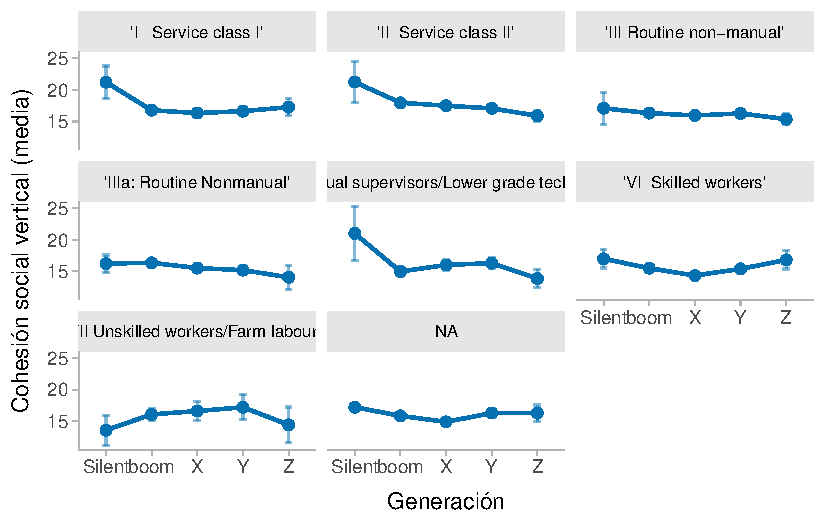
\includegraphics[keepaspectratio]{procesamiento/descriptivo_bivariado_files/figure-pdf/grafico-clase-generacion-1.pdf}}

\begin{Shaded}
\begin{Highlighting}[]
\NormalTok{grafico\_clase\_gen\_path }\OtherTok{\textless{}{-}} \FunctionTok{file.path}\NormalTok{(output\_graphs\_dir, }\StringTok{"cohesion\_clase\_generacion.png"}\NormalTok{)}
\ControlFlowTok{if}\NormalTok{ (}\SpecialCharTok{!}\FunctionTok{file.exists}\NormalTok{(grafico\_clase\_gen\_path)) \{}
  \FunctionTok{ggsave}\NormalTok{(}\AttributeTok{filename =}\NormalTok{ grafico\_clase\_gen\_path, }\AttributeTok{plot =}\NormalTok{ grafico\_clase\_gen,}
         \AttributeTok{width =} \DecValTok{8}\NormalTok{, }\AttributeTok{height =} \DecValTok{6}\NormalTok{, }\AttributeTok{dpi =} \DecValTok{300}\NormalTok{)}
\NormalTok{\}}
\end{Highlighting}
\end{Shaded}

\section{Evolución temporal de la cohesión
vertical}\label{evoluciuxf3n-temporal-de-la-cohesiuxf3n-vertical}

Se examina la trayectoria promedio de la cohesión social vertical a lo
largo de las siete olas, con intervalos de confianza. Este gráfico
permite identificar los efectos de los shocks contextuales (estallido
social 2019, pandemia 2020--2022).

\begin{Shaded}
\begin{Highlighting}[]
\NormalTok{resumen\_ola }\OtherTok{\textless{}{-}}\NormalTok{ data\_f }\SpecialCharTok{\%\textgreater{}\%}
  \FunctionTok{group\_by}\NormalTok{(ola) }\SpecialCharTok{\%\textgreater{}\%}
  \FunctionTok{summarise}\NormalTok{(}
    \AttributeTok{media   =} \FunctionTok{mean}\NormalTok{(c05\_total, }\AttributeTok{na.rm =} \ConstantTok{TRUE}\NormalTok{),}
    \AttributeTok{se      =} \FunctionTok{sd}\NormalTok{(c05\_total, }\AttributeTok{na.rm =} \ConstantTok{TRUE}\NormalTok{) }\SpecialCharTok{/} \FunctionTok{sqrt}\NormalTok{(}\FunctionTok{n}\NormalTok{()),}
    \AttributeTok{.groups =} \StringTok{"drop"}
\NormalTok{  ) }\SpecialCharTok{\%\textgreater{}\%}
  \FunctionTok{mutate}\NormalTok{(}
    \AttributeTok{ci\_low  =}\NormalTok{ media }\SpecialCharTok{{-}} \FloatTok{1.96} \SpecialCharTok{*}\NormalTok{ se,}
    \AttributeTok{ci\_high =}\NormalTok{ media }\SpecialCharTok{+} \FloatTok{1.96} \SpecialCharTok{*}\NormalTok{ se}
\NormalTok{  )}

\NormalTok{grafico\_temporal }\OtherTok{\textless{}{-}}\NormalTok{ resumen\_ola }\SpecialCharTok{\%\textgreater{}\%}
  \FunctionTok{ggplot}\NormalTok{(}\FunctionTok{aes}\NormalTok{(}\AttributeTok{x =}\NormalTok{ ola, }\AttributeTok{y =}\NormalTok{ media, }\AttributeTok{group =} \DecValTok{1}\NormalTok{)) }\SpecialCharTok{+}
  \FunctionTok{geom\_ribbon}\NormalTok{(}\FunctionTok{aes}\NormalTok{(}\AttributeTok{ymin =}\NormalTok{ ci\_low, }\AttributeTok{ymax =}\NormalTok{ ci\_high), }\AttributeTok{alpha =} \FloatTok{0.2}\NormalTok{, }\AttributeTok{fill =} \StringTok{"\#0571B0"}\NormalTok{) }\SpecialCharTok{+}
  \FunctionTok{geom\_line}\NormalTok{(}\AttributeTok{linewidth =} \DecValTok{1}\NormalTok{, }\AttributeTok{color =} \StringTok{"\#0571B0"}\NormalTok{) }\SpecialCharTok{+}
  \FunctionTok{geom\_point}\NormalTok{(}\AttributeTok{size =} \DecValTok{3}\NormalTok{, }\AttributeTok{color =} \StringTok{"\#0571B0"}\NormalTok{) }\SpecialCharTok{+}
  \FunctionTok{annotate}\NormalTok{(}\StringTok{"rect"}\NormalTok{, }\AttributeTok{xmin =} \FloatTok{3.5}\NormalTok{, }\AttributeTok{xmax =} \FloatTok{5.5}\NormalTok{, }\AttributeTok{ymin =} \SpecialCharTok{{-}}\ConstantTok{Inf}\NormalTok{, }\AttributeTok{ymax =} \ConstantTok{Inf}\NormalTok{,}
           \AttributeTok{alpha =} \FloatTok{0.1}\NormalTok{, }\AttributeTok{fill =} \StringTok{"red"}\NormalTok{) }\SpecialCharTok{+}
  \FunctionTok{annotate}\NormalTok{(}\StringTok{"text"}\NormalTok{, }\AttributeTok{x =} \FloatTok{4.5}\NormalTok{, }\AttributeTok{y =} \FunctionTok{max}\NormalTok{(resumen\_ola}\SpecialCharTok{$}\NormalTok{ci\_high),}
           \AttributeTok{label =} \StringTok{"Estallido + Pandemia"}\NormalTok{, }\AttributeTok{size =} \DecValTok{3}\NormalTok{, }\AttributeTok{color =} \StringTok{"red"}\NormalTok{) }\SpecialCharTok{+}
  \FunctionTok{labs}\NormalTok{(}
    \AttributeTok{x =} \StringTok{"Ola de medición"}\NormalTok{,}
    \AttributeTok{y =} \StringTok{"Cohesión social vertical (media)"}
\NormalTok{  ) }\SpecialCharTok{+}
  \FunctionTok{theme\_ggdist}\NormalTok{(}\AttributeTok{base\_size =} \DecValTok{16}\NormalTok{) }\SpecialCharTok{+}
  \FunctionTok{theme}\NormalTok{(}
    \AttributeTok{axis.title =} \FunctionTok{element\_text}\NormalTok{(}\AttributeTok{size =} \DecValTok{16}\NormalTok{),}
    \AttributeTok{axis.text  =} \FunctionTok{element\_text}\NormalTok{(}\AttributeTok{size =} \DecValTok{14}\NormalTok{),}
    \AttributeTok{plot.title =} \FunctionTok{element\_text}\NormalTok{(}\AttributeTok{size =} \DecValTok{18}\NormalTok{)}
\NormalTok{  )}

\NormalTok{grafico\_temporal}
\end{Highlighting}
\end{Shaded}

\pandocbounded{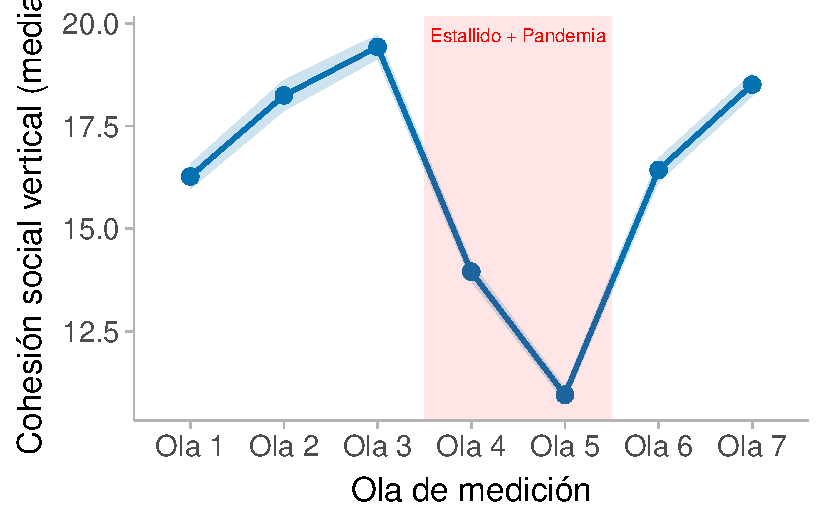
\includegraphics[keepaspectratio]{procesamiento/descriptivo_bivariado_files/figure-pdf/grafico-temporal-1.pdf}}

\begin{Shaded}
\begin{Highlighting}[]
\FunctionTok{ggsave}\NormalTok{(}\FunctionTok{file.path}\NormalTok{(output\_graphs\_dir, }\StringTok{"cohesion\_temporal.png"}\NormalTok{),}
       \AttributeTok{plot =}\NormalTok{ grafico\_temporal, }\AttributeTok{width =} \DecValTok{8}\NormalTok{, }\AttributeTok{height =} \DecValTok{5}\NormalTok{, }\AttributeTok{dpi =} \DecValTok{300}\NormalTok{)}
\end{Highlighting}
\end{Shaded}

\section{Cohesión vertical por nivel
educativo}\label{cohesiuxf3n-vertical-por-nivel-educativo}

Se examina la distribución de la cohesión social vertical según nivel
educativo, para explorar el gradiente educativo antes de la modelación.

\begin{Shaded}
\begin{Highlighting}[]
\NormalTok{resumen\_nedu }\OtherTok{\textless{}{-}}\NormalTok{ data\_f }\SpecialCharTok{\%\textgreater{}\%}
  \FunctionTok{filter}\NormalTok{(}\SpecialCharTok{!}\FunctionTok{is.na}\NormalTok{(nedu)) }\SpecialCharTok{\%\textgreater{}\%}
  \FunctionTok{group\_by}\NormalTok{(nedu) }\SpecialCharTok{\%\textgreater{}\%}
  \FunctionTok{summarise}\NormalTok{(}
    \AttributeTok{media   =} \FunctionTok{mean}\NormalTok{(c05\_total, }\AttributeTok{na.rm =} \ConstantTok{TRUE}\NormalTok{),}
    \AttributeTok{se      =} \FunctionTok{sd}\NormalTok{(c05\_total, }\AttributeTok{na.rm =} \ConstantTok{TRUE}\NormalTok{) }\SpecialCharTok{/} \FunctionTok{sqrt}\NormalTok{(}\FunctionTok{n}\NormalTok{()),}
    \AttributeTok{n       =} \FunctionTok{n}\NormalTok{(),}
    \AttributeTok{.groups =} \StringTok{"drop"}
\NormalTok{  ) }\SpecialCharTok{\%\textgreater{}\%}
  \FunctionTok{mutate}\NormalTok{(}
    \AttributeTok{ci\_low  =}\NormalTok{ media }\SpecialCharTok{{-}} \FloatTok{1.96} \SpecialCharTok{*}\NormalTok{ se,}
    \AttributeTok{ci\_high =}\NormalTok{ media }\SpecialCharTok{+} \FloatTok{1.96} \SpecialCharTok{*}\NormalTok{ se}
\NormalTok{  )}

\NormalTok{grafico\_nedu }\OtherTok{\textless{}{-}}\NormalTok{ resumen\_nedu }\SpecialCharTok{\%\textgreater{}\%}
  \FunctionTok{ggplot}\NormalTok{(}\FunctionTok{aes}\NormalTok{(}\AttributeTok{x =}\NormalTok{ nedu, }\AttributeTok{y =}\NormalTok{ media)) }\SpecialCharTok{+}
  \FunctionTok{geom\_col}\NormalTok{(}\AttributeTok{fill =} \StringTok{"\#0571B0"}\NormalTok{, }\AttributeTok{alpha =} \FloatTok{0.8}\NormalTok{) }\SpecialCharTok{+}
  \FunctionTok{geom\_errorbar}\NormalTok{(}\FunctionTok{aes}\NormalTok{(}\AttributeTok{ymin =}\NormalTok{ ci\_low, }\AttributeTok{ymax =}\NormalTok{ ci\_high),}
                \AttributeTok{width =} \FloatTok{0.2}\NormalTok{, }\AttributeTok{color =} \StringTok{"gray30"}\NormalTok{) }\SpecialCharTok{+}
  \FunctionTok{geom\_text}\NormalTok{(}\FunctionTok{aes}\NormalTok{(}\AttributeTok{label =} \FunctionTok{paste0}\NormalTok{(}\StringTok{"n="}\NormalTok{, n)), }\AttributeTok{vjust =} \SpecialCharTok{{-}}\FloatTok{1.5}\NormalTok{, }\AttributeTok{size =} \DecValTok{3}\NormalTok{) }\SpecialCharTok{+}
  \FunctionTok{labs}\NormalTok{(}
    \AttributeTok{x =} \StringTok{"Nivel educativo"}\NormalTok{,}
    \AttributeTok{y =} \StringTok{"Cohesión social vertical (media)"}
\NormalTok{  ) }\SpecialCharTok{+}
  \FunctionTok{theme\_ggdist}\NormalTok{(}\AttributeTok{base\_size =} \DecValTok{14}\NormalTok{) }\SpecialCharTok{+}
  \FunctionTok{theme}\NormalTok{(}
    \AttributeTok{axis.title =} \FunctionTok{element\_text}\NormalTok{(}\AttributeTok{size =} \DecValTok{14}\NormalTok{),}
    \AttributeTok{axis.text  =} \FunctionTok{element\_text}\NormalTok{(}\AttributeTok{size =} \DecValTok{12}\NormalTok{),}
    \AttributeTok{plot.title =} \FunctionTok{element\_text}\NormalTok{(}\AttributeTok{size =} \DecValTok{18}\NormalTok{)}
\NormalTok{  )}

\NormalTok{grafico\_nedu}
\end{Highlighting}
\end{Shaded}

\pandocbounded{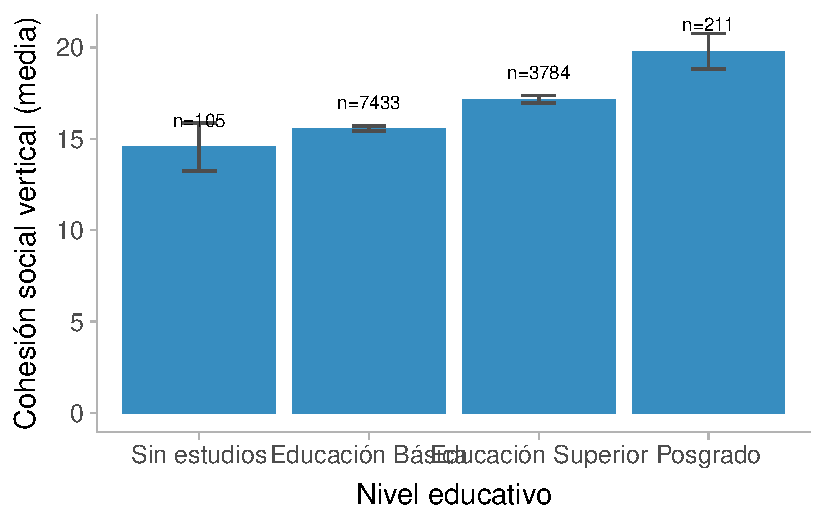
\includegraphics[keepaspectratio]{procesamiento/descriptivo_bivariado_files/figure-pdf/grafico-educacion-1.pdf}}

\begin{Shaded}
\begin{Highlighting}[]
\FunctionTok{ggsave}\NormalTok{(}\FunctionTok{file.path}\NormalTok{(output\_graphs\_dir, }\StringTok{"cohesion\_educacion.png"}\NormalTok{),}
       \AttributeTok{plot =}\NormalTok{ grafico\_nedu, }\AttributeTok{width =} \DecValTok{7}\NormalTok{, }\AttributeTok{height =} \DecValTok{5}\NormalTok{, }\AttributeTok{dpi =} \DecValTok{300}\NormalTok{)}
\end{Highlighting}
\end{Shaded}

\section{Cohesión vertical por percepción de
corrupción}\label{cohesiuxf3n-vertical-por-percepciuxf3n-de-corrupciuxf3n}

Se examina si existe un gradiente en la cohesión vertical según el nivel
de percepción de corrupción institucional, tanto en su versión
categórica como continua.

\begin{Shaded}
\begin{Highlighting}[]
\NormalTok{resumen\_c38 }\OtherTok{\textless{}{-}}\NormalTok{ data\_f }\SpecialCharTok{\%\textgreater{}\%}
  \FunctionTok{filter}\NormalTok{(}\SpecialCharTok{!}\FunctionTok{is.na}\NormalTok{(c38\_cat)) }\SpecialCharTok{\%\textgreater{}\%}
  \FunctionTok{group\_by}\NormalTok{(c38\_cat) }\SpecialCharTok{\%\textgreater{}\%}
  \FunctionTok{summarise}\NormalTok{(}
    \AttributeTok{media   =} \FunctionTok{mean}\NormalTok{(c05\_total, }\AttributeTok{na.rm =} \ConstantTok{TRUE}\NormalTok{),}
    \AttributeTok{se      =} \FunctionTok{sd}\NormalTok{(c05\_total, }\AttributeTok{na.rm =} \ConstantTok{TRUE}\NormalTok{) }\SpecialCharTok{/} \FunctionTok{sqrt}\NormalTok{(}\FunctionTok{n}\NormalTok{()),}
    \AttributeTok{n       =} \FunctionTok{n}\NormalTok{(),}
    \AttributeTok{.groups =} \StringTok{"drop"}
\NormalTok{  ) }\SpecialCharTok{\%\textgreater{}\%}
  \FunctionTok{mutate}\NormalTok{(}
    \AttributeTok{ci\_low  =}\NormalTok{ media }\SpecialCharTok{{-}} \FloatTok{1.96} \SpecialCharTok{*}\NormalTok{ se,}
    \AttributeTok{ci\_high =}\NormalTok{ media }\SpecialCharTok{+} \FloatTok{1.96} \SpecialCharTok{*}\NormalTok{ se}
\NormalTok{  )}

\NormalTok{grafico\_c38 }\OtherTok{\textless{}{-}}\NormalTok{ resumen\_c38 }\SpecialCharTok{\%\textgreater{}\%}
  \FunctionTok{ggplot}\NormalTok{(}\FunctionTok{aes}\NormalTok{(}\AttributeTok{x =}\NormalTok{ c38\_cat, }\AttributeTok{y =}\NormalTok{ media)) }\SpecialCharTok{+}
  \FunctionTok{geom\_col}\NormalTok{(}\AttributeTok{fill =} \StringTok{"\#CA0020"}\NormalTok{, }\AttributeTok{alpha =} \FloatTok{0.8}\NormalTok{) }\SpecialCharTok{+}
  \FunctionTok{geom\_errorbar}\NormalTok{(}\FunctionTok{aes}\NormalTok{(}\AttributeTok{ymin =}\NormalTok{ ci\_low, }\AttributeTok{ymax =}\NormalTok{ ci\_high),}
                \AttributeTok{width =} \FloatTok{0.2}\NormalTok{, }\AttributeTok{color =} \StringTok{"gray30"}\NormalTok{) }\SpecialCharTok{+}
  \FunctionTok{geom\_text}\NormalTok{(}\FunctionTok{aes}\NormalTok{(}\AttributeTok{label =} \FunctionTok{paste0}\NormalTok{(}\StringTok{"n="}\NormalTok{, n)), }\AttributeTok{vjust =} \SpecialCharTok{{-}}\FloatTok{1.5}\NormalTok{, }\AttributeTok{size =} \DecValTok{3}\NormalTok{) }\SpecialCharTok{+}
  \FunctionTok{labs}\NormalTok{(}
    \AttributeTok{x =} \StringTok{"Percepción de corrupción"}\NormalTok{,}
    \AttributeTok{y =} \StringTok{"Cohesión social vertical (media)"}
\NormalTok{  ) }\SpecialCharTok{+}
  \FunctionTok{theme\_ggdist}\NormalTok{(}\AttributeTok{base\_size =} \DecValTok{16}\NormalTok{) }\SpecialCharTok{+}                                     \CommentTok{\# \textless{}{-} aumenta esto para ejes/etiquetas}
  \FunctionTok{theme}\NormalTok{(}
    \AttributeTok{axis.title =} \FunctionTok{element\_text}\NormalTok{(}\AttributeTok{size =} \DecValTok{16}\NormalTok{),}
    \AttributeTok{axis.text  =} \FunctionTok{element\_text}\NormalTok{(}\AttributeTok{size =} \DecValTok{14}\NormalTok{),}
    \AttributeTok{plot.title =} \FunctionTok{element\_text}\NormalTok{(}\AttributeTok{size =} \DecValTok{18}\NormalTok{)}
\NormalTok{  )}


\NormalTok{grafico\_c38}
\end{Highlighting}
\end{Shaded}

\pandocbounded{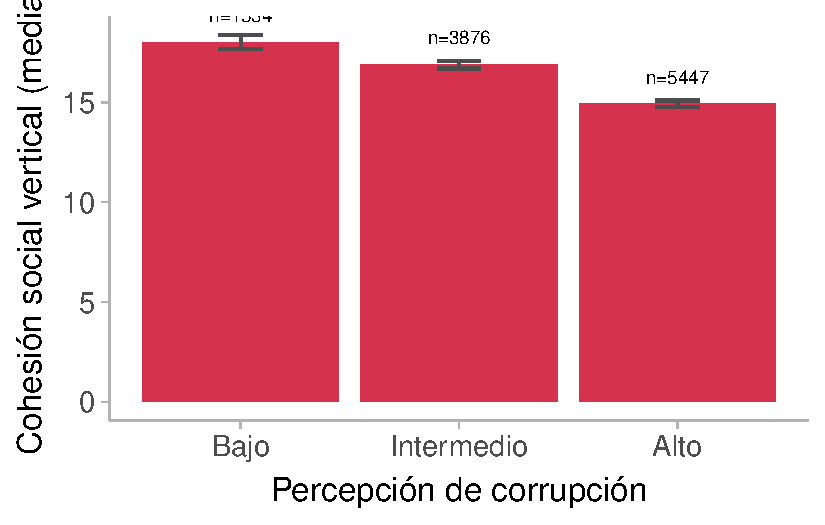
\includegraphics[keepaspectratio]{procesamiento/descriptivo_bivariado_files/figure-pdf/grafico-corrupcion-1.pdf}}

\begin{Shaded}
\begin{Highlighting}[]
\FunctionTok{ggsave}\NormalTok{(}\FunctionTok{file.path}\NormalTok{(output\_graphs\_dir, }\StringTok{"cohesion\_corrupcion.png"}\NormalTok{),}
       \AttributeTok{plot =}\NormalTok{ grafico\_c38, }\AttributeTok{width =} \DecValTok{7}\NormalTok{, }\AttributeTok{height =} \DecValTok{5}\NormalTok{, }\AttributeTok{dpi =} \DecValTok{300}\NormalTok{)}
\end{Highlighting}
\end{Shaded}

\section{Cohesión vertical por percepción de
meritocracia}\label{cohesiuxf3n-vertical-por-percepciuxf3n-de-meritocracia}

Se examina la relación entre la percepción de meritocracia y la cohesión
vertical, tanto en su versión categórica como a través de la evolución
temporal por nivel de meritocracia.

\begin{Shaded}
\begin{Highlighting}[]
\NormalTok{resumen\_c32 }\OtherTok{\textless{}{-}}\NormalTok{ data\_f }\SpecialCharTok{\%\textgreater{}\%}
  \FunctionTok{filter}\NormalTok{(}\SpecialCharTok{!}\FunctionTok{is.na}\NormalTok{(c32\_cat)) }\SpecialCharTok{\%\textgreater{}\%}
  \FunctionTok{group\_by}\NormalTok{(c32\_cat) }\SpecialCharTok{\%\textgreater{}\%}
  \FunctionTok{summarise}\NormalTok{(}
    \AttributeTok{media   =} \FunctionTok{mean}\NormalTok{(c05\_total, }\AttributeTok{na.rm =} \ConstantTok{TRUE}\NormalTok{),}
    \AttributeTok{se      =} \FunctionTok{sd}\NormalTok{(c05\_total, }\AttributeTok{na.rm =} \ConstantTok{TRUE}\NormalTok{) }\SpecialCharTok{/} \FunctionTok{sqrt}\NormalTok{(}\FunctionTok{n}\NormalTok{()),}
    \AttributeTok{n       =} \FunctionTok{n}\NormalTok{(),}
    \AttributeTok{.groups =} \StringTok{"drop"}
\NormalTok{  ) }\SpecialCharTok{\%\textgreater{}\%}
  \FunctionTok{mutate}\NormalTok{(}
    \AttributeTok{ci\_low  =}\NormalTok{ media }\SpecialCharTok{{-}} \FloatTok{1.96} \SpecialCharTok{*}\NormalTok{ se,}
    \AttributeTok{ci\_high =}\NormalTok{ media }\SpecialCharTok{+} \FloatTok{1.96} \SpecialCharTok{*}\NormalTok{ se}
\NormalTok{  )}

\NormalTok{grafico\_c32 }\OtherTok{\textless{}{-}}\NormalTok{ resumen\_c32 }\SpecialCharTok{\%\textgreater{}\%}
  \FunctionTok{ggplot}\NormalTok{(}\FunctionTok{aes}\NormalTok{(}\AttributeTok{x =}\NormalTok{ c32\_cat, }\AttributeTok{y =}\NormalTok{ media)) }\SpecialCharTok{+}
  \FunctionTok{geom\_col}\NormalTok{(}\AttributeTok{fill =} \StringTok{"\#1A9641"}\NormalTok{, }\AttributeTok{alpha =} \FloatTok{0.8}\NormalTok{) }\SpecialCharTok{+}
  \FunctionTok{geom\_errorbar}\NormalTok{(}\FunctionTok{aes}\NormalTok{(}\AttributeTok{ymin =}\NormalTok{ ci\_low, }\AttributeTok{ymax =}\NormalTok{ ci\_high),}
                \AttributeTok{width =} \FloatTok{0.2}\NormalTok{, }\AttributeTok{color =} \StringTok{"gray30"}\NormalTok{) }\SpecialCharTok{+}
  \FunctionTok{geom\_text}\NormalTok{(}\FunctionTok{aes}\NormalTok{(}\AttributeTok{label =} \FunctionTok{paste0}\NormalTok{(}\StringTok{"n="}\NormalTok{, n)), }\AttributeTok{vjust =} \SpecialCharTok{{-}}\FloatTok{1.5}\NormalTok{, }\AttributeTok{size =} \DecValTok{3}\NormalTok{) }\SpecialCharTok{+}
  \FunctionTok{labs}\NormalTok{(}
    \AttributeTok{x =} \StringTok{"Identificación nacional"}\NormalTok{,}
    \AttributeTok{y =} \StringTok{"Cohesión social vertical (media)"}
\NormalTok{  ) }\SpecialCharTok{+}
  \FunctionTok{theme\_ggdist}\NormalTok{(}\AttributeTok{base\_size =} \DecValTok{16}\NormalTok{) }\SpecialCharTok{+}                                     \CommentTok{\# \textless{}{-} aumenta esto para ejes/etiquetas}
  \FunctionTok{theme}\NormalTok{(}
    \AttributeTok{axis.title =} \FunctionTok{element\_text}\NormalTok{(}\AttributeTok{size =} \DecValTok{16}\NormalTok{),}
    \AttributeTok{axis.text  =} \FunctionTok{element\_text}\NormalTok{(}\AttributeTok{size =} \DecValTok{14}\NormalTok{),}
    \AttributeTok{plot.title =} \FunctionTok{element\_text}\NormalTok{(}\AttributeTok{size =} \DecValTok{18}\NormalTok{)}
\NormalTok{  )}


\NormalTok{grafico\_c32}
\end{Highlighting}
\end{Shaded}

\pandocbounded{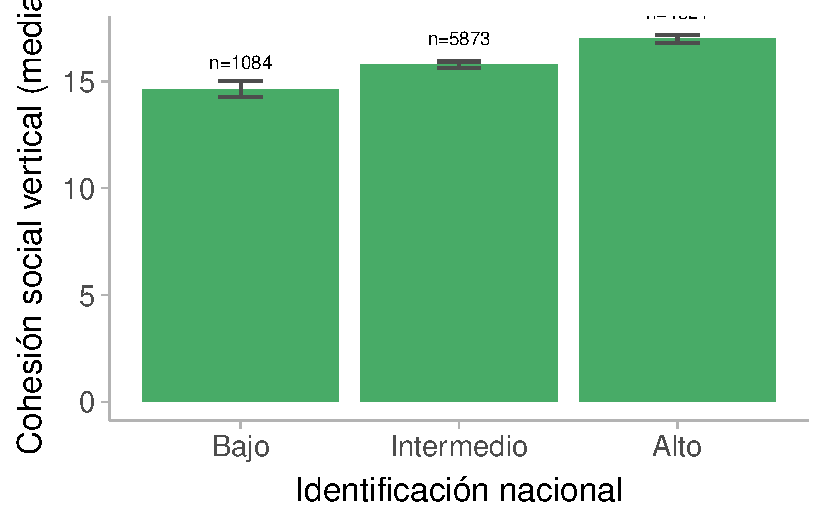
\includegraphics[keepaspectratio]{procesamiento/descriptivo_bivariado_files/figure-pdf/grafico-identificacion-1.pdf}}

\begin{Shaded}
\begin{Highlighting}[]
\FunctionTok{ggsave}\NormalTok{(}\FunctionTok{file.path}\NormalTok{(output\_graphs\_dir, }\StringTok{"cohesion\_meritocracia.png"}\NormalTok{),}
       \AttributeTok{plot =}\NormalTok{ grafico\_c32, }\AttributeTok{width =} \DecValTok{7}\NormalTok{, }\AttributeTok{height =} \DecValTok{5}\NormalTok{, }\AttributeTok{dpi =} \DecValTok{300}\NormalTok{)}
\end{Highlighting}
\end{Shaded}

\section{Evolución temporal por
generación}\label{evoluciuxf3n-temporal-por-generaciuxf3n}

Se examina si las trayectorias temporales de la cohesión vertical
difieren entre cohortes generacionales, lo que permite explorar efectos
de interacción generación × tiempo antes de la modelación.

\begin{Shaded}
\begin{Highlighting}[]
\NormalTok{resumen\_ola\_gen }\OtherTok{\textless{}{-}}\NormalTok{ data\_f }\SpecialCharTok{\%\textgreater{}\%}
  \FunctionTok{filter}\NormalTok{(}\SpecialCharTok{!}\FunctionTok{is.na}\NormalTok{(Generacion)) }\SpecialCharTok{\%\textgreater{}\%}
  \FunctionTok{group\_by}\NormalTok{(ola, Generacion) }\SpecialCharTok{\%\textgreater{}\%}
  \FunctionTok{summarise}\NormalTok{(}
    \AttributeTok{media   =} \FunctionTok{mean}\NormalTok{(c05\_total, }\AttributeTok{na.rm =} \ConstantTok{TRUE}\NormalTok{),}
    \AttributeTok{se      =} \FunctionTok{sd}\NormalTok{(c05\_total, }\AttributeTok{na.rm =} \ConstantTok{TRUE}\NormalTok{) }\SpecialCharTok{/} \FunctionTok{sqrt}\NormalTok{(}\FunctionTok{n}\NormalTok{()),}
    \AttributeTok{.groups =} \StringTok{"drop"}
\NormalTok{  ) }\SpecialCharTok{\%\textgreater{}\%}
  \FunctionTok{mutate}\NormalTok{(}
    \AttributeTok{ci\_low  =}\NormalTok{ media }\SpecialCharTok{{-}} \FloatTok{1.96} \SpecialCharTok{*}\NormalTok{ se,}
    \AttributeTok{ci\_high =}\NormalTok{ media }\SpecialCharTok{+} \FloatTok{1.96} \SpecialCharTok{*}\NormalTok{ se}
\NormalTok{  )}

\NormalTok{grafico\_ola\_gen }\OtherTok{\textless{}{-}}\NormalTok{ resumen\_ola\_gen }\SpecialCharTok{\%\textgreater{}\%}
  \FunctionTok{ggplot}\NormalTok{(}\FunctionTok{aes}\NormalTok{(}\AttributeTok{x =}\NormalTok{ ola, }\AttributeTok{y =}\NormalTok{ media, }\AttributeTok{color =}\NormalTok{ Generacion, }\AttributeTok{group =}\NormalTok{ Generacion)) }\SpecialCharTok{+}
  \FunctionTok{geom\_ribbon}\NormalTok{(}\FunctionTok{aes}\NormalTok{(}\AttributeTok{ymin =}\NormalTok{ ci\_low, }\AttributeTok{ymax =}\NormalTok{ ci\_high, }\AttributeTok{fill =}\NormalTok{ Generacion),}
              \AttributeTok{alpha =} \FloatTok{0.1}\NormalTok{, }\AttributeTok{color =} \ConstantTok{NA}\NormalTok{) }\SpecialCharTok{+}
  \FunctionTok{geom\_line}\NormalTok{(}\AttributeTok{linewidth =} \FloatTok{0.9}\NormalTok{) }\SpecialCharTok{+}
  \FunctionTok{geom\_point}\NormalTok{(}\AttributeTok{size =} \DecValTok{2}\NormalTok{) }\SpecialCharTok{+}
  \FunctionTok{scale\_color\_brewer}\NormalTok{(}\AttributeTok{palette =} \StringTok{"Set1"}\NormalTok{) }\SpecialCharTok{+}
  \FunctionTok{scale\_fill\_brewer}\NormalTok{(}\AttributeTok{palette =} \StringTok{"Set1"}\NormalTok{) }\SpecialCharTok{+}
  \FunctionTok{labs}\NormalTok{(}
    \AttributeTok{x =} \StringTok{"Ola de medición"}\NormalTok{,}
    \AttributeTok{y =} \StringTok{"Cohesión social vertical (media)"}\NormalTok{,}
    \AttributeTok{color =} \StringTok{"Generación"}\NormalTok{,}
    \AttributeTok{fill  =} \StringTok{"Generación"}
\NormalTok{  ) }\SpecialCharTok{+}
  \FunctionTok{theme\_ggdist}\NormalTok{(}\AttributeTok{base\_size =} \DecValTok{16}\NormalTok{) }\SpecialCharTok{+} 
  \FunctionTok{theme}\NormalTok{(}
    \AttributeTok{axis.title =} \FunctionTok{element\_text}\NormalTok{(}\AttributeTok{size =} \DecValTok{16}\NormalTok{),}
    \AttributeTok{axis.text  =} \FunctionTok{element\_text}\NormalTok{(}\AttributeTok{size =} \DecValTok{14}\NormalTok{),}
    \AttributeTok{plot.title =} \FunctionTok{element\_text}\NormalTok{(}\AttributeTok{size =} \DecValTok{18}\NormalTok{)}
\NormalTok{  ) }\SpecialCharTok{+}
  \FunctionTok{theme}\NormalTok{(}\AttributeTok{legend.position =} \StringTok{"bottom"}\NormalTok{)}

\NormalTok{grafico\_ola\_gen}
\end{Highlighting}
\end{Shaded}

\pandocbounded{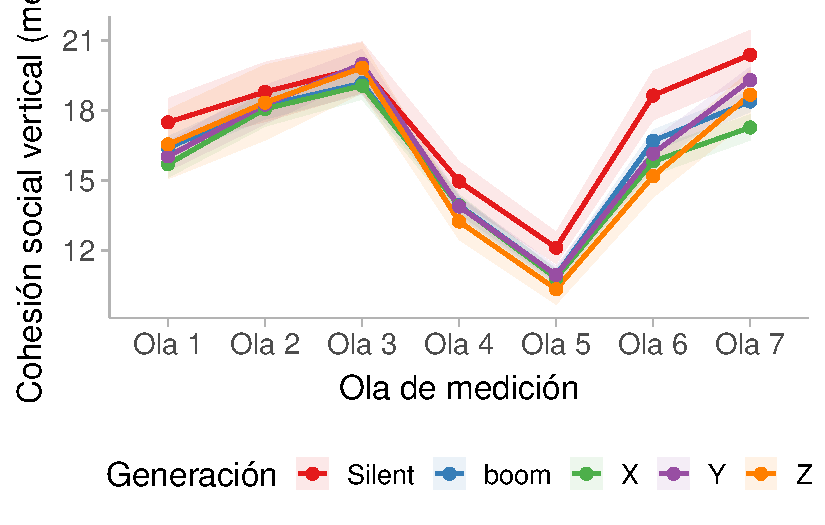
\includegraphics[keepaspectratio]{procesamiento/descriptivo_bivariado_files/figure-pdf/grafico-temporal-generacion-1.pdf}}

\begin{Shaded}
\begin{Highlighting}[]
\FunctionTok{ggsave}\NormalTok{(}\FunctionTok{file.path}\NormalTok{(output\_graphs\_dir, }\StringTok{"cohesion\_temporal\_generacion.png"}\NormalTok{),}
       \AttributeTok{plot =}\NormalTok{ grafico\_ola\_gen, }\AttributeTok{width =} \DecValTok{9}\NormalTok{, }\AttributeTok{height =} \DecValTok{6}\NormalTok{, }\AttributeTok{dpi =} \DecValTok{300}\NormalTok{)}
\end{Highlighting}
\end{Shaded}

\section{Evolución temporal por clase
social}\label{evoluciuxf3n-temporal-por-clase-social}

De forma análoga, se examina si las trayectorias temporales difieren
entre clases sociales (EGP-4).

\begin{Shaded}
\begin{Highlighting}[]
\NormalTok{resumen\_ola\_clase }\OtherTok{\textless{}{-}}\NormalTok{ data\_f }\SpecialCharTok{\%\textgreater{}\%}
  \FunctionTok{filter}\NormalTok{(}\SpecialCharTok{!}\FunctionTok{is.na}\NormalTok{(egp4)) }\SpecialCharTok{\%\textgreater{}\%}
  \FunctionTok{group\_by}\NormalTok{(ola, egp4) }\SpecialCharTok{\%\textgreater{}\%}
  \FunctionTok{summarise}\NormalTok{(}
    \AttributeTok{media   =} \FunctionTok{mean}\NormalTok{(c05\_total, }\AttributeTok{na.rm =} \ConstantTok{TRUE}\NormalTok{),}
    \AttributeTok{se      =} \FunctionTok{sd}\NormalTok{(c05\_total, }\AttributeTok{na.rm =} \ConstantTok{TRUE}\NormalTok{) }\SpecialCharTok{/} \FunctionTok{sqrt}\NormalTok{(}\FunctionTok{n}\NormalTok{()),}
    \AttributeTok{.groups =} \StringTok{"drop"}
\NormalTok{  ) }\SpecialCharTok{\%\textgreater{}\%}
  \FunctionTok{mutate}\NormalTok{(}
    \AttributeTok{ci\_low  =}\NormalTok{ media }\SpecialCharTok{{-}} \FloatTok{1.96} \SpecialCharTok{*}\NormalTok{ se,}
    \AttributeTok{ci\_high =}\NormalTok{ media }\SpecialCharTok{+} \FloatTok{1.96} \SpecialCharTok{*}\NormalTok{ se}
\NormalTok{  )}

\NormalTok{grafico\_ola\_clase }\OtherTok{\textless{}{-}}\NormalTok{ resumen\_ola\_clase }\SpecialCharTok{\%\textgreater{}\%}
  \FunctionTok{ggplot}\NormalTok{(}\FunctionTok{aes}\NormalTok{(}\AttributeTok{x =}\NormalTok{ ola, }\AttributeTok{y =}\NormalTok{ media, }\AttributeTok{color =}\NormalTok{ egp4, }\AttributeTok{group =}\NormalTok{ egp4)) }\SpecialCharTok{+}
  \FunctionTok{geom\_ribbon}\NormalTok{(}\FunctionTok{aes}\NormalTok{(}\AttributeTok{ymin =}\NormalTok{ ci\_low, }\AttributeTok{ymax =}\NormalTok{ ci\_high, }\AttributeTok{fill =}\NormalTok{ egp4),}
              \AttributeTok{alpha =} \FloatTok{0.1}\NormalTok{, }\AttributeTok{color =} \ConstantTok{NA}\NormalTok{) }\SpecialCharTok{+}
  \FunctionTok{geom\_line}\NormalTok{(}\AttributeTok{linewidth =} \FloatTok{0.9}\NormalTok{) }\SpecialCharTok{+}
  \FunctionTok{geom\_point}\NormalTok{(}\AttributeTok{size =} \DecValTok{2}\NormalTok{) }\SpecialCharTok{+}
  \FunctionTok{scale\_color\_brewer}\NormalTok{(}\AttributeTok{palette =} \StringTok{"Dark2"}\NormalTok{) }\SpecialCharTok{+}
  \FunctionTok{scale\_fill\_brewer}\NormalTok{(}\AttributeTok{palette =} \StringTok{"Dark2"}\NormalTok{) }\SpecialCharTok{+}
  \FunctionTok{labs}\NormalTok{(    }\AttributeTok{x =} \StringTok{"Ola de medición"}\NormalTok{,}
    \AttributeTok{y =} \StringTok{"Cohesión social vertical (media)"}\NormalTok{,}
    \AttributeTok{color =} \StringTok{"Clase social"}\NormalTok{,}
    \AttributeTok{fill  =} \StringTok{"Clase social"}
\NormalTok{  ) }\SpecialCharTok{+}
  \FunctionTok{theme\_ggdist}\NormalTok{(}\AttributeTok{base\_size =} \DecValTok{16}
\NormalTok{  ) }\SpecialCharTok{+}                                     \CommentTok{\# \textless{}{-} aumenta esto para ejes/etiquetas}
  \FunctionTok{theme}\NormalTok{(}
    \AttributeTok{axis.title =} \FunctionTok{element\_text}\NormalTok{(}\AttributeTok{size =} \DecValTok{16}\NormalTok{),}
    \AttributeTok{axis.text  =} \FunctionTok{element\_text}\NormalTok{(}\AttributeTok{size =} \DecValTok{14}\NormalTok{),}
    \AttributeTok{plot.title =} \FunctionTok{element\_text}\NormalTok{(}\AttributeTok{size =} \DecValTok{18}\NormalTok{)}
\NormalTok{  ) }\SpecialCharTok{+}
  \FunctionTok{theme}\NormalTok{(}\AttributeTok{legend.position =} \StringTok{"bottom"}\NormalTok{)}

\NormalTok{grafico\_ola\_clase}
\end{Highlighting}
\end{Shaded}

\pandocbounded{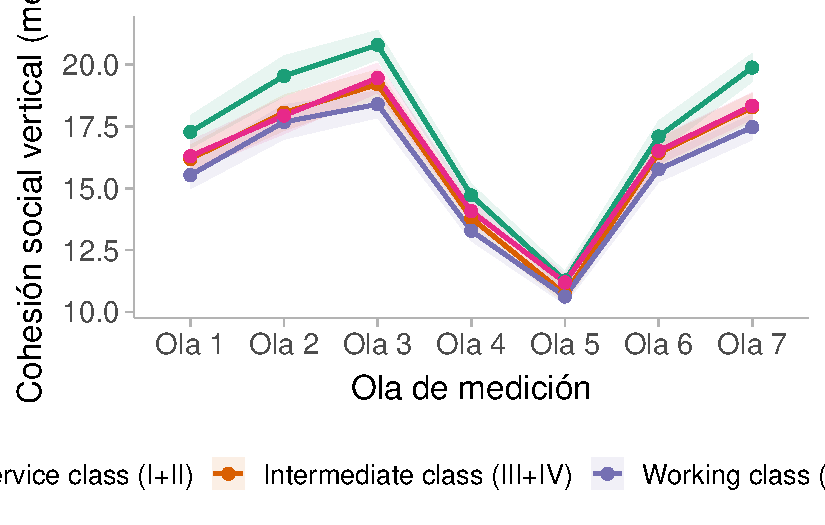
\includegraphics[keepaspectratio]{procesamiento/descriptivo_bivariado_files/figure-pdf/grafico-temporal-clase-1.pdf}}

\begin{Shaded}
\begin{Highlighting}[]
\FunctionTok{ggsave}\NormalTok{(}\FunctionTok{file.path}\NormalTok{(output\_graphs\_dir, }\StringTok{"cohesion\_temporal\_clase.png"}\NormalTok{),}
       \AttributeTok{plot =}\NormalTok{ grafico\_ola\_clase, }\AttributeTok{width =} \DecValTok{9}\NormalTok{, }\AttributeTok{height =} \DecValTok{6}\NormalTok{, }\AttributeTok{dpi =} \DecValTok{300}\NormalTok{)}
\end{Highlighting}
\end{Shaded}

\section{Distribución de la variable
dependiente}\label{distribuciuxf3n-de-la-variable-dependiente}

Se examina la distribución de \texttt{c05\_total} para evaluar su forma
y detectar posibles asimetrías o valores extremos relevantes para la
modelación.

\begin{Shaded}
\begin{Highlighting}[]
\NormalTok{grafico\_dist }\OtherTok{\textless{}{-}}\NormalTok{ data\_f }\SpecialCharTok{\%\textgreater{}\%}
  \FunctionTok{ggplot}\NormalTok{(}\FunctionTok{aes}\NormalTok{(}\AttributeTok{x =}\NormalTok{ c05\_total)) }\SpecialCharTok{+}
  \FunctionTok{geom\_histogram}\NormalTok{(}\AttributeTok{binwidth =} \DecValTok{1}\NormalTok{, }\AttributeTok{fill =} \StringTok{"\#0571B0"}\NormalTok{, }\AttributeTok{color =} \StringTok{"white"}\NormalTok{, }\AttributeTok{alpha =} \FloatTok{0.8}\NormalTok{) }\SpecialCharTok{+}
  \FunctionTok{geom\_vline}\NormalTok{(}\AttributeTok{xintercept =} \FunctionTok{mean}\NormalTok{(data\_f}\SpecialCharTok{$}\NormalTok{c05\_total, }\AttributeTok{na.rm =} \ConstantTok{TRUE}\NormalTok{),}
             \AttributeTok{color =} \StringTok{"red"}\NormalTok{, }\AttributeTok{linetype =} \StringTok{"dashed"}\NormalTok{, }\AttributeTok{linewidth =} \FloatTok{0.8}\NormalTok{) }\SpecialCharTok{+}
  \FunctionTok{annotate}\NormalTok{(}\StringTok{"text"}\NormalTok{,}
           \AttributeTok{x =} \FunctionTok{mean}\NormalTok{(data\_f}\SpecialCharTok{$}\NormalTok{c05\_total, }\AttributeTok{na.rm =} \ConstantTok{TRUE}\NormalTok{) }\SpecialCharTok{+} \FloatTok{0.5}\NormalTok{,}
           \AttributeTok{y =} \ConstantTok{Inf}\NormalTok{, }\AttributeTok{vjust =} \DecValTok{2}\NormalTok{,}
           \AttributeTok{label =} \FunctionTok{paste0}\NormalTok{(}\StringTok{"Media = "}\NormalTok{, }\FunctionTok{round}\NormalTok{(}\FunctionTok{mean}\NormalTok{(data\_f}\SpecialCharTok{$}\NormalTok{c05\_total, }\AttributeTok{na.rm =} \ConstantTok{TRUE}\NormalTok{), }\DecValTok{2}\NormalTok{)),}
           \AttributeTok{color =} \StringTok{"red"}\NormalTok{, }\AttributeTok{size =} \FloatTok{3.5}\NormalTok{) }\SpecialCharTok{+}
  \FunctionTok{labs}\NormalTok{(}
    \AttributeTok{x =} \StringTok{"Cohesión social vertical (c05\_total)"}\NormalTok{,}
    \AttributeTok{y =} \StringTok{"Frecuencia"}
\NormalTok{  ) }\SpecialCharTok{+}
  \FunctionTok{theme\_ggdist}\NormalTok{()}

\NormalTok{grafico\_dist}
\end{Highlighting}
\end{Shaded}

\pandocbounded{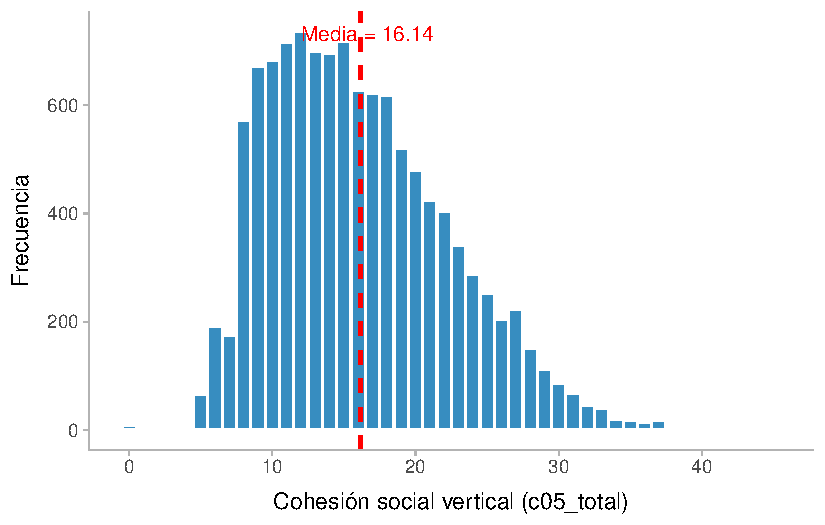
\includegraphics[keepaspectratio]{procesamiento/descriptivo_bivariado_files/figure-pdf/grafico-distribucion-dv-1.pdf}}

\begin{Shaded}
\begin{Highlighting}[]
\FunctionTok{ggsave}\NormalTok{(}\FunctionTok{file.path}\NormalTok{(output\_graphs\_dir, }\StringTok{"distribucion\_dv.png"}\NormalTok{),}
       \AttributeTok{plot =}\NormalTok{ grafico\_dist, }\AttributeTok{width =} \DecValTok{7}\NormalTok{, }\AttributeTok{height =} \DecValTok{5}\NormalTok{, }\AttributeTok{dpi =} \DecValTok{300}\NormalTok{)}
\end{Highlighting}
\end{Shaded}

\chapter{Análisis Multinivel}\label{anuxe1lisis-multinivel}

Cohesión Social Vertical en Chile (2016--2023)

\hfill\break

\begin{Shaded}
\begin{Highlighting}[]
\NormalTok{label\_map }\OtherTok{\textless{}{-}} \FunctionTok{c}\NormalTok{(}
  \StringTok{"(Intercept)"}            \OtherTok{=} \StringTok{"Intercept"}\NormalTok{,}
  
  \CommentTok{\# Corruption perception}
  \StringTok{"c38"}                    \OtherTok{=} \StringTok{"Corruption perception"}\NormalTok{,}
  \StringTok{"c38\_grand"}              \OtherTok{=} \StringTok{"Corruption perception (Grand{-}mean centered)"}\NormalTok{,}
  \StringTok{"c38\_within"}             \OtherTok{=} \StringTok{"Corruption perception (Specific{-}mean centered)"}\NormalTok{,}
  \StringTok{"c38\_between"}            \OtherTok{=} \StringTok{"Corruption perception (Person historical mean)"}\NormalTok{,}
  \StringTok{"c38\_within:c38\_between"} \OtherTok{=} \StringTok{"Corruption perception (Cross{-}level Interaction)"}\NormalTok{,}
  \StringTok{"c38\_catIntermedio"}      \OtherTok{=} \StringTok{"Corruption perception: Intermediate"}\NormalTok{,}
  \StringTok{"c38\_catAlto"}            \OtherTok{=} \StringTok{"Corruption perception: High"}\NormalTok{,}

  \CommentTok{\# Age}
  \StringTok{"m0\_edad"}                \OtherTok{=} \StringTok{"Age"}\NormalTok{,}
  \StringTok{"m0\_edad\_grand"}          \OtherTok{=} \StringTok{"Age (Grand{-}mean centered)"}\NormalTok{,}
  \StringTok{"m0\_edad\_within"}         \OtherTok{=} \StringTok{"Age (Specific{-}mean centered)"}\NormalTok{,}
  \StringTok{"m0\_edad\_between"}        \OtherTok{=} \StringTok{"Age (Person historical mean)"}\NormalTok{,}
  \StringTok{"m0\_edad\_within:m0\_edad\_between"} \OtherTok{=} \StringTok{"Interaction: Age (within) × Age (between)"}\NormalTok{,}

  \CommentTok{\# Meritocracy / National identification}
  \StringTok{"c32\_01\_ord"}             \OtherTok{=} \StringTok{"Meritocracy perception"}\NormalTok{,}
  \StringTok{"c32\_01\_ord.L"}           \OtherTok{=} \StringTok{"Meritocracy perception (Linear trend)"}\NormalTok{,}
  \StringTok{"c32\_01\_ord.Q"}           \OtherTok{=} \StringTok{"Meritocracy perception (Quadratic trend)"}\NormalTok{,}
  \StringTok{"c32\_01\_ord.C"}           \OtherTok{=} \StringTok{"Meritocracy perception (Cubic trend)"}\NormalTok{,}
  \StringTok{"c32\_01\_ord\^{}4"}           \OtherTok{=} \StringTok{"Meritocracy perception (4th degree trend)"}\NormalTok{,}
  \StringTok{"c32\_grand"}              \OtherTok{=} \StringTok{"National identification (Grand{-}mean centered)"}\NormalTok{,}
  \StringTok{"c32\_within"}             \OtherTok{=} \StringTok{"National identification (Specific{-}mean centered)"}\NormalTok{,}
  \StringTok{"c32\_between"}            \OtherTok{=} \StringTok{"National identification (Person historical mean)"}\NormalTok{,}
  \StringTok{"c32\_catIntermedio"}      \OtherTok{=} \StringTok{"National identification: Intermediate"}\NormalTok{,}
  \StringTok{"c32\_catAlto"}            \OtherTok{=} \StringTok{"National identification: High"}\NormalTok{,}

  \CommentTok{\# Dignified treatment}
  \StringTok{"trato\_digno"}            \OtherTok{=} \StringTok{"Dignified treatment"}\NormalTok{,}
  \StringTok{"trato\_digno\_grand"}      \OtherTok{=} \StringTok{"Dignified treatment (Grand{-}mean centered)"}\NormalTok{,}
  \StringTok{"trato\_digno\_within"}     \OtherTok{=} \StringTok{"Dignified treatment (Specific{-}mean centered)"}\NormalTok{,}
  \StringTok{"trato\_digno\_between"}    \OtherTok{=} \StringTok{"Dignified treatment (Person historical mean)"}\NormalTok{,}

  \CommentTok{\# Political self{-}identification}
  \StringTok{"c15"}                    \OtherTok{=} \StringTok{"Political self{-}identification"}\NormalTok{,}
  \StringTok{"c15\_grand"}              \OtherTok{=} \StringTok{"Political self{-}identification (Grand{-}mean centered)"}\NormalTok{,}
  \StringTok{"c15\_within"}             \OtherTok{=} \StringTok{"Political self{-}identification (Specific{-}mean centered)"}\NormalTok{,}
  \StringTok{"c15\_between"}            \OtherTok{=} \StringTok{"Political self{-}identification (Person historical mean)"}\NormalTok{,}

  \CommentTok{\# Indigenous self{-}identification}
  \StringTok{"indigena"}               \OtherTok{=} \StringTok{"Indigenous self{-}identification"}\NormalTok{,}

  \CommentTok{\# Sex \& Education}
  \StringTok{"sexoMujer"}              \OtherTok{=} \StringTok{"Sex: Female"}\NormalTok{,}
  \StringTok{"neduEducación Básica"}   \OtherTok{=} \StringTok{"Education: Basic"}\NormalTok{,}
  \StringTok{"neduEducación Superior"} \OtherTok{=} \StringTok{"Education: Higher education"}\NormalTok{,}
  \StringTok{"neduPosgrado"}           \OtherTok{=} \StringTok{"Education: Postgraduate"}\NormalTok{,}

  \CommentTok{\# Generation (ref. = Silent)}
  \StringTok{"Generacionboom"}         \OtherTok{=} \StringTok{"Generation: Boom"}\NormalTok{,}
  \StringTok{"GeneracionX"}            \OtherTok{=} \StringTok{"Generation: X"}\NormalTok{,}
  \StringTok{"GeneracionY"}            \OtherTok{=} \StringTok{"Generation: Y"}\NormalTok{,}
  \StringTok{"GeneracionZ"}            \OtherTok{=} \StringTok{"Generation: Z"}\NormalTok{,}

  \CommentTok{\# Social class EGP{-}7 (ref. = Service class I)}
  \StringTok{"egp7\textquotesingle{}II  Service class II\textquotesingle{}"}                           \OtherTok{=} \StringTok{"Service class II"}\NormalTok{,}
  \StringTok{"egp7\textquotesingle{}III Routine non{-}manual\textquotesingle{}"}                         \OtherTok{=} \StringTok{"Routine non{-}manual"}\NormalTok{,}
  \StringTok{"egp7\textquotesingle{}IIIa: Routine Nonmanual\textquotesingle{}"}                        \OtherTok{=} \StringTok{"Routine non{-}manual (IIIa)"}\NormalTok{,}
  \StringTok{"egp7\textquotesingle{}V   Manual supervisors/Lower grade technicians\textquotesingle{}"} \OtherTok{=} \StringTok{"Manual supervisors"}\NormalTok{,}
  \StringTok{"egp7\textquotesingle{}VI  Skilled workers\textquotesingle{}"}                            \OtherTok{=} \StringTok{"Skilled workers"}\NormalTok{,}
  \StringTok{"egp7\textquotesingle{}VII Unskilled workers/Farm labours\textquotesingle{}"}             \OtherTok{=} \StringTok{"Unskilled workers"}\NormalTok{,}

  \CommentTok{\# Social class EGP{-}4 (ref. = Service class I+II)}
  \StringTok{"egp4Intermediate class (III+IV)"}                    \OtherTok{=} \StringTok{"Intermediate class (III+IV)"}\NormalTok{,}
  \StringTok{"egp4Working class (V+VI+VII)"}                       \OtherTok{=} \StringTok{"Working class (V+VI+VII)"}\NormalTok{,}
  \StringTok{"egp4Out of labor force"}                             \OtherTok{=} \StringTok{"Out of labor force"}\NormalTok{,}

  \CommentTok{\# Wave (ref. = Ola 1 / 2016)}
  \StringTok{"olaOla 2"} \OtherTok{=} \StringTok{"Wave 2017"}\NormalTok{,}
  \StringTok{"olaOla 3"} \OtherTok{=} \StringTok{"Wave 2018"}\NormalTok{,}
  \StringTok{"olaOla 4"} \OtherTok{=} \StringTok{"Wave 2019"}\NormalTok{,}
  \StringTok{"olaOla 5"} \OtherTok{=} \StringTok{"Wave 2021"}\NormalTok{,}
  \StringTok{"olaOla 6"} \OtherTok{=} \StringTok{"Wave 2022"}\NormalTok{,}
  \StringTok{"olaOla 7"} \OtherTok{=} \StringTok{"Wave 2023"}\NormalTok{,}

  \CommentTok{\# DV}
  \StringTok{"c05\_total"} \OtherTok{=} \StringTok{"Organizational participation (DV)"}\NormalTok{,}

  \CommentTok{\# Interacciones edad within x clase social EGP{-}4}
  \StringTok{"m0\_edad\_within:egp4Intermediate class (III+IV)"}    \OtherTok{=} \StringTok{"Age (within) × Intermediate class"}\NormalTok{,}
  \StringTok{"m0\_edad\_within:egp4Working class (V+VI+VII)"}       \OtherTok{=} \StringTok{"Age (within) × Working class"}\NormalTok{,}
  \StringTok{"m0\_edad\_within:egp4Out of labor force"}             \OtherTok{=} \StringTok{"Age (within) × Out of labor force"}
\NormalTok{) }
\end{Highlighting}
\end{Shaded}

\chapter{Presentación}\label{presentaciuxf3n-2}

Este documento presenta la estimación de modelos lineales mixtos
(\emph{Linear Mixed Models}, LMM) para el análisis de la cohesión social
vertical en Chile entre 2016 y 2023. Se sigue una estrategia de
modelación progresiva, partiendo de un modelo nulo y añadiendo
predictores de forma incremental. Todas las variables continuas se
utilizan en su versión centrada: las variables que capturan variación
intraindividual se centran en la media del propio individuo
(\emph{within-person centering}), y las variables que capturan
diferencias estables entre individuos se incluyen como promedios
individuales (\emph{between-person means}). Esta descomposición permite
separar los efectos dentro y entre individuos en el marco de un diseño
longitudinal.

\chapter{Librerías y datos}\label{libreruxedas-y-datos-1}

\begin{Shaded}
\begin{Highlighting}[]
\FunctionTok{library}\NormalTok{(haven)}
\FunctionTok{library}\NormalTok{(here)}
\FunctionTok{library}\NormalTok{(lme4)}
\FunctionTok{library}\NormalTok{(lmerTest)}
\FunctionTok{library}\NormalTok{(performance)}
\FunctionTok{library}\NormalTok{(psych)}
\FunctionTok{library}\NormalTok{(texreg)}
\FunctionTok{library}\NormalTok{(modelsummary)}
\FunctionTok{library}\NormalTok{(dplyr)}

\NormalTok{output\_tables\_dir }\OtherTok{\textless{}{-}} \FunctionTok{file.path}\NormalTok{(}\StringTok{"output"}\NormalTok{, }\StringTok{"tables"}\NormalTok{)}
\FunctionTok{dir.create}\NormalTok{(output\_tables\_dir, }\AttributeTok{recursive =} \ConstantTok{TRUE}\NormalTok{, }\AttributeTok{showWarnings =} \ConstantTok{FALSE}\NormalTok{)}

\NormalTok{data          }\OtherTok{\textless{}{-}} \FunctionTok{readRDS}\NormalTok{(}\FunctionTok{here}\NormalTok{(}\StringTok{"input/data\_regresion.rds"}\NormalTok{))}
\NormalTok{data\_f        }\OtherTok{\textless{}{-}} \FunctionTok{readRDS}\NormalTok{(}\FunctionTok{here}\NormalTok{(}\StringTok{"input/data\_f\_regresion.rds"}\NormalTok{))}
\NormalTok{data\_centrada }\OtherTok{\textless{}{-}} \FunctionTok{readRDS}\NormalTok{(}\FunctionTok{here}\NormalTok{(}\StringTok{"input/data\_centrada\_regresion.rds"}\NormalTok{))}
\end{Highlighting}
\end{Shaded}

\chapter{Preparación de la muestra
analítica}\label{preparaciuxf3n-de-la-muestra-analuxedtica}

\section{Centrado de variables
adicionales}\label{centrado-de-variables-adicionales}

Se reconstruyen las versiones centradas de \texttt{c32} (percepción de
meritocracia) que no fueron guardadas en el archivo procesado, dado que
esta variable requiere conversión numérica previa desde su formato
ordinal.

\begin{Shaded}
\begin{Highlighting}[]
\NormalTok{data\_centrada }\OtherTok{\textless{}{-}}\NormalTok{ data\_centrada }\SpecialCharTok{\%\textgreater{}\%}
  \FunctionTok{mutate}\NormalTok{(}\AttributeTok{c32\_01\_ord =} \FunctionTok{as.factor}\NormalTok{(c32\_01\_ord)) }\SpecialCharTok{\%\textgreater{}\%}
  \FunctionTok{mutate}\NormalTok{(}\AttributeTok{c32\_num =} \FunctionTok{as.numeric}\NormalTok{(}\FunctionTok{as.character}\NormalTok{(c32\_01\_ord))) }\SpecialCharTok{\%\textgreater{}\%}
  \FunctionTok{mutate}\NormalTok{(}\AttributeTok{c32\_grand =}\NormalTok{ c32\_num }\SpecialCharTok{{-}} \FunctionTok{mean}\NormalTok{(c32\_num, }\AttributeTok{na.rm =} \ConstantTok{TRUE}\NormalTok{)) }\SpecialCharTok{\%\textgreater{}\%}
  \FunctionTok{group\_by}\NormalTok{(idencuesta) }\SpecialCharTok{\%\textgreater{}\%}
  \FunctionTok{mutate}\NormalTok{(}
    \AttributeTok{c32\_within  =}\NormalTok{ c32\_num }\SpecialCharTok{{-}} \FunctionTok{mean}\NormalTok{(c32\_num, }\AttributeTok{na.rm =} \ConstantTok{TRUE}\NormalTok{),}
    \AttributeTok{c32\_between =} \FunctionTok{mean}\NormalTok{(c32\_num, }\AttributeTok{na.rm =} \ConstantTok{TRUE}\NormalTok{)}
\NormalTok{  ) }\SpecialCharTok{\%\textgreater{}\%}
  \FunctionTok{ungroup}\NormalTok{()}
\end{Highlighting}
\end{Shaded}

\section{Restricción a muestra
homogénea}\label{restricciuxf3n-a-muestra-homoguxe9nea}

Para garantizar que todos los modelos se estimen sobre la misma muestra,
se restringe \texttt{data\_centrada} a los casos con información
completa en todas las variables utilizadas. Esto evita que las
comparaciones de ajuste entre modelos estén contaminadas por diferencias
en el tamaño muestral.

\begin{Shaded}
\begin{Highlighting}[]
\NormalTok{data\_centrada }\OtherTok{\textless{}{-}}\NormalTok{ data\_centrada }\SpecialCharTok{\%\textgreater{}\%}
  \FunctionTok{filter}\NormalTok{(}\FunctionTok{complete.cases}\NormalTok{(.))}

\FunctionTok{cat}\NormalTok{(}\StringTok{"N observaciones (muestra homogénea):"}\NormalTok{, }\FunctionTok{nrow}\NormalTok{(data\_centrada), }\StringTok{"}\SpecialCharTok{\textbackslash{}n}\StringTok{"}\NormalTok{)}
\end{Highlighting}
\end{Shaded}

\begin{verbatim}
N observaciones (muestra homogénea): 7979 
\end{verbatim}

\begin{Shaded}
\begin{Highlighting}[]
\FunctionTok{cat}\NormalTok{(}\StringTok{"N individuos:"}\NormalTok{, }\FunctionTok{n\_distinct}\NormalTok{(data\_centrada}\SpecialCharTok{$}\NormalTok{idencuesta), }\StringTok{"}\SpecialCharTok{\textbackslash{}n}\StringTok{"}\NormalTok{)}
\end{Highlighting}
\end{Shaded}

\begin{verbatim}
N individuos: 1372 
\end{verbatim}

\chapter{Consistencia interna}\label{consistencia-interna}

Antes de la estimación de modelos, se verifica la consistencia interna
de la escala de trato digno (\texttt{c35\_01} a \texttt{c35\_03})
mediante el coeficiente alpha de Cronbach. Un alpha satisfactorio
justifica el uso del índice aditivo como indicador único en los modelos.

\begin{Shaded}
\begin{Highlighting}[]
\NormalTok{alpha\_trato\_digno }\OtherTok{\textless{}{-}}\NormalTok{ data }\SpecialCharTok{\%\textgreater{}\%}
  \FunctionTok{select}\NormalTok{(c35\_01}\SpecialCharTok{:}\NormalTok{c35\_03) }\SpecialCharTok{\%\textgreater{}\%}
\NormalTok{  psych}\SpecialCharTok{::}\FunctionTok{alpha}\NormalTok{()}

\NormalTok{alpha\_trato\_digno}
\end{Highlighting}
\end{Shaded}

\begin{verbatim}

Reliability analysis   
Call: psych::alpha(x = .)

  raw_alpha std.alpha G6(smc) average_r S/N    ase mean   sd median_r
      0.77      0.78     0.7      0.54 3.5 0.0037  3.3 0.96     0.55

    95% confidence boundaries 
         lower alpha upper
Feldt     0.77  0.77  0.78
Duhachek  0.77  0.77  0.78

 Reliability if an item is dropped:
       raw_alpha std.alpha G6(smc) average_r S/N alpha se var.r med.r
c35_01      0.70      0.71    0.55      0.55 2.4   0.0055    NA  0.55
c35_02      0.64      0.64    0.47      0.47 1.8   0.0066    NA  0.47
c35_03      0.74      0.74    0.59      0.59 2.8   0.0049    NA  0.59

 Item statistics 
          n raw.r std.r r.cor r.drop mean  sd
c35_01 5574  0.82  0.83  0.69   0.60  3.1 1.1
c35_02 5514  0.85  0.86  0.75   0.66  3.4 1.1
c35_03 5530  0.82  0.81  0.65   0.57  3.3 1.2

Non missing response frequency for each item
          1    2    3    4    5 miss
c35_01 0.10 0.16 0.40 0.20 0.13 0.52
c35_02 0.07 0.11 0.39 0.25 0.18 0.52
c35_03 0.10 0.12 0.34 0.24 0.21 0.52
\end{verbatim}

\chapter{Estimación de modelos}\label{estimaciuxf3n-de-modelos}

\section{Modelo nulo e ICC}\label{modelo-nulo-e-icc}

El modelo nulo sin predictores permite estimar la Correlación Intraclase
(ICC), que cuantifica qué proporción de la varianza total en
participación organizacional es atribuible a diferencias estables entre
individuos. Una ICC elevada justifica el uso de modelos multinivel.

\begin{Shaded}
\begin{Highlighting}[]
\NormalTok{model\_0\_cent }\OtherTok{\textless{}{-}} \FunctionTok{lmer}\NormalTok{(c05\_total }\SpecialCharTok{\textasciitilde{}}\NormalTok{ (}\DecValTok{1} \SpecialCharTok{|}\NormalTok{ idencuesta), }\AttributeTok{data =}\NormalTok{ data\_centrada)}
\NormalTok{performance}\SpecialCharTok{::}\FunctionTok{icc}\NormalTok{(model\_0\_cent)}
\end{Highlighting}
\end{Shaded}

\begin{verbatim}
# Intraclass Correlation Coefficient

    Adjusted ICC: 0.289
  Unadjusted ICC: 0.289
\end{verbatim}

\begin{Shaded}
\begin{Highlighting}[]
\NormalTok{performance}\SpecialCharTok{::}\FunctionTok{r2}\NormalTok{(model\_0\_cent)}
\end{Highlighting}
\end{Shaded}

\begin{verbatim}
# R2 for Mixed Models

  Conditional R2: 0.289
     Marginal R2: 0.000
\end{verbatim}

\section{Modelo temporal}\label{modelo-temporal}

Se incorpora únicamente la ola de medición como predictor, capturando la
tendencia agregada de la participación a lo largo del tiempo antes de
introducir predictores sustantivos.

\begin{Shaded}
\begin{Highlighting}[]
\NormalTok{model\_temp\_cent }\OtherTok{\textless{}{-}} \FunctionTok{lmer}\NormalTok{(c05\_total }\SpecialCharTok{\textasciitilde{}}\NormalTok{ ola }\SpecialCharTok{+}\NormalTok{ (}\DecValTok{1} \SpecialCharTok{|}\NormalTok{ idencuesta), }\AttributeTok{data =}\NormalTok{ data\_centrada)}
\FunctionTok{summary}\NormalTok{(model\_temp\_cent)}
\end{Highlighting}
\end{Shaded}

\begin{verbatim}
Linear mixed model fit by REML. t-tests use Satterthwaite's method [
lmerModLmerTest]
Formula: c05_total ~ ola + (1 | idencuesta)
   Data: data_centrada

REML criterion at convergence: 48331.8

Scaled residuals: 
    Min      1Q  Median      3Q     Max 
-3.7100 -0.6185 -0.0492  0.5635  5.8476 

Random effects:
 Groups     Name        Variance Std.Dev.
 idencuesta (Intercept) 12.20    3.492   
 Residual               19.24    4.386   
Number of obs: 7979, groups:  idencuesta, 1372

Fixed effects:
             Estimate Std. Error        df t value Pr(>|t|)    
(Intercept)   15.7106     0.1803 6290.1718  87.156  < 2e-16 ***
olaOla 2       2.1133     0.2100 6636.4369  10.061  < 2e-16 ***
olaOla 3       3.7192     0.1954 6807.5655  19.031  < 2e-16 ***
olaOla 4      -1.7999     0.1945 6808.5554  -9.256  < 2e-16 ***
olaOla 5      -4.8659     0.1952 6812.0648 -24.925  < 2e-16 ***
olaOla 6       0.7121     0.1948 6810.9543   3.656 0.000259 ***
olaOla 7       3.0427     0.2100 6638.2035  14.491  < 2e-16 ***
---
Signif. codes:  0 '***' 0.001 '**' 0.01 '*' 0.05 '.' 0.1 ' ' 1

Correlation of Fixed Effects:
         (Intr) olaOl2 olaOl3 olaOl4 olaOl5 olaOl6
olaOla 2 -0.587                                   
olaOla 3 -0.669  0.541                            
olaOla 4 -0.673  0.544  0.620                     
olaOla 5 -0.670  0.541  0.618  0.621              
olaOla 6 -0.672  0.543  0.619  0.622  0.620       
olaOla 7 -0.587  0.504  0.541  0.544  0.542  0.544
\end{verbatim}

\begin{Shaded}
\begin{Highlighting}[]
\NormalTok{performance}\SpecialCharTok{::}\FunctionTok{r2}\NormalTok{(model\_temp\_cent)}
\end{Highlighting}
\end{Shaded}

\begin{verbatim}
# R2 for Mixed Models

  Conditional R2: 0.516
     Marginal R2: 0.210
\end{verbatim}

\section{Modelo 1: predictores actitudinales (efectos
within)}\label{modelo-1-predictores-actitudinales-efectos-within}

Se introducen los predictores actitudinales en su versión
\emph{within-person} (desviación respecto a la media individual) para
capturar los cambios intraindividuales a lo largo del tiempo. Las
variables cuya variación es principalmente entre individuos se incluyen
como promedios individuales (\emph{between}).

\begin{Shaded}
\begin{Highlighting}[]
\NormalTok{model\_1\_cent }\OtherTok{\textless{}{-}} \FunctionTok{lmer}\NormalTok{(c05\_total }\SpecialCharTok{\textasciitilde{}} 
\NormalTok{                       c38\_within }\SpecialCharTok{+}
\NormalTok{                       m0\_edad\_within }\SpecialCharTok{+}
\NormalTok{                       trato\_digno\_within }\SpecialCharTok{+}
\NormalTok{                       c15\_within }\SpecialCharTok{+}
\NormalTok{                       c32\_within }\SpecialCharTok{+}
\NormalTok{                       Generacion }\SpecialCharTok{+} 
\NormalTok{                       (}\DecValTok{1} \SpecialCharTok{|}\NormalTok{ idencuesta), }\AttributeTok{data =}\NormalTok{ data\_centrada)}
\FunctionTok{summary}\NormalTok{(model\_1\_cent)}
\end{Highlighting}
\end{Shaded}

\begin{verbatim}
Linear mixed model fit by REML. t-tests use Satterthwaite's method [
lmerModLmerTest]
Formula: c05_total ~ c38_within + m0_edad_within + trato_digno_within +  
    c15_within + c32_within + Generacion + (1 | idencuesta)
   Data: data_centrada

REML criterion at convergence: 50899.6

Scaled residuals: 
    Min      1Q  Median      3Q     Max 
-3.5280 -0.6910 -0.1035  0.6032  5.3131 

Random effects:
 Groups     Name        Variance Std.Dev.
 idencuesta (Intercept) 11.67    3.416   
 Residual               27.95    5.287   
Number of obs: 7979, groups:  idencuesta, 1372

Fixed effects:
                     Estimate Std. Error         df t value Pr(>|t|)    
(Intercept)          17.91454    0.68170 1306.92084  26.279  < 2e-16 ***
c38_within           -0.46688    0.09027 6659.69731  -5.172 2.39e-07 ***
m0_edad_within        0.07160    0.02759 6714.74232   2.596 0.009462 ** 
trato_digno_within    0.16695    0.01607 6694.49090  10.390  < 2e-16 ***
c15_within           -0.03537    0.02017 6703.48881  -1.753 0.079581 .  
c32_within            0.67356    0.10020 6712.24743   6.722 1.94e-11 ***
Generacionboom       -1.89262    0.70475 1309.85940  -2.686 0.007333 ** 
GeneracionX          -2.32261    0.71448 1312.41168  -3.251 0.001180 ** 
GeneracionY          -2.01220    0.71702 1315.72273  -2.806 0.005085 ** 
GeneracionZ          -2.66105    0.78778 1344.04833  -3.378 0.000751 ***
---
Signif. codes:  0 '***' 0.001 '**' 0.01 '*' 0.05 '.' 0.1 ' ' 1

Correlation of Fixed Effects:
            (Intr) c38_wt m0_dd_ trt_d_ c15_wt c32_wt Gnrcnb GnrcnX GnrcnY
c38_within   0.001                                                        
m0_edd_wthn  0.002 -0.051                                                 
trt_dgn_wth  0.002  0.047  0.475                                          
c15_within  -0.001 -0.018  0.050 -0.006                                   
c32_within   0.001  0.001  0.018 -0.047  0.021                            
Generacinbm -0.967 -0.001  0.003  0.001  0.001 -0.001                     
GeneracionX -0.954 -0.001  0.004  0.002  0.001 -0.002  0.923              
GeneracionY -0.951 -0.002  0.006  0.003  0.001  0.000  0.920  0.907       
GeneracionZ -0.865 -0.001  0.007  0.004  0.000  0.001  0.837  0.826  0.823
\end{verbatim}

\begin{Shaded}
\begin{Highlighting}[]
\NormalTok{performance}\SpecialCharTok{::}\FunctionTok{r2}\NormalTok{(model\_1\_cent)}
\end{Highlighting}
\end{Shaded}

\begin{verbatim}
# R2 for Mixed Models

  Conditional R2: 0.310
     Marginal R2: 0.022
\end{verbatim}

\section{Modelo 2: predictores estructurales y
between}\label{modelo-2-predictores-estructurales-y-between}

Se incorporan los predictores estructurales de nivel individual
(generación, clase social, sexo, nivel educativo) junto con los
promedios individuales de las variables actitudinales, capturando las
diferencias estables entre individuos.

\begin{Shaded}
\begin{Highlighting}[]
\NormalTok{model\_2\_cent }\OtherTok{\textless{}{-}} \FunctionTok{lmer}\NormalTok{(c05\_total }\SpecialCharTok{\textasciitilde{}} 
\NormalTok{                       Generacion }\SpecialCharTok{+}\NormalTok{ egp4 }\SpecialCharTok{+}\NormalTok{ sexo }\SpecialCharTok{+}\NormalTok{ nedu }\SpecialCharTok{+}
\NormalTok{                       c38\_between }\SpecialCharTok{+}\NormalTok{ m0\_edad\_between }\SpecialCharTok{+}
\NormalTok{                       trato\_digno\_between }\SpecialCharTok{+}\NormalTok{ c15\_between }\SpecialCharTok{+}\NormalTok{ c32\_between }\SpecialCharTok{+}
\NormalTok{                       (}\DecValTok{1} \SpecialCharTok{|}\NormalTok{ idencuesta), }\AttributeTok{data =}\NormalTok{ data\_centrada)}
\FunctionTok{summary}\NormalTok{(model\_2\_cent)}
\end{Highlighting}
\end{Shaded}

\begin{verbatim}
Linear mixed model fit by REML. t-tests use Satterthwaite's method [
lmerModLmerTest]
Formula: 
c05_total ~ Generacion + egp4 + sexo + nedu + c38_between + m0_edad_between +  
    trato_digno_between + c15_between + c32_between + (1 | idencuesta)
   Data: data_centrada

REML criterion at convergence: 50704.5

Scaled residuals: 
    Min      1Q  Median      3Q     Max 
-3.5393 -0.6940 -0.1019  0.6270  5.1930 

Random effects:
 Groups     Name        Variance Std.Dev.
 idencuesta (Intercept)  7.386   2.718   
 Residual               28.811   5.368   
Number of obs: 7979, groups:  idencuesta, 1372

Fixed effects:
                                  Estimate Std. Error         df t value
(Intercept)                       22.85846    2.31757 1678.13589   9.863
Generacionboom                    -1.08936    0.69939 1306.11084  -1.558
GeneracionX                       -1.37790    0.89721 1323.66723  -1.536
GeneracionY                       -1.19941    1.11085 1330.55201  -1.080
GeneracionZ                       -1.62487    1.33111 1340.98420  -1.221
egp4Intermediate class (III+IV)   -0.58484    0.20258 5144.94466  -2.887
egp4Working class (V+VI+VII)      -0.93001    0.21333 4085.49098  -4.360
sexoMujer                         -0.04748    0.19987 1440.53873  -0.238
neduEducación Básica               0.96775    0.99689 5209.28213   0.971
neduEducación Superior             2.22082    1.01307 5138.59187   2.192
neduPosgrado                       3.78210    1.14220 5234.19866   3.311
c38_between                       -2.11320    0.16647 1369.03937 -12.694
m0_edad_between                    0.01469    0.02282 1355.67724   0.644
trato_digno_between               -0.30911    0.03007 1673.33013 -10.281
c15_between                       -0.28075    0.03872 1431.43930  -7.251
c32_between                        1.22132    0.19988 1455.10459   6.110
                                Pr(>|t|)    
(Intercept)                      < 2e-16 ***
Generacionboom                  0.119577    
GeneracionX                     0.124839    
GeneracionY                     0.280460    
GeneracionZ                     0.222419    
egp4Intermediate class (III+IV) 0.003906 ** 
egp4Working class (V+VI+VII)    1.34e-05 ***
sexoMujer                       0.812244    
neduEducación Básica            0.331709    
neduEducación Superior          0.028412 *  
neduPosgrado                    0.000935 ***
c38_between                      < 2e-16 ***
m0_edad_between                 0.519867    
trato_digno_between              < 2e-16 ***
c15_between                     6.76e-13 ***
c32_between                     1.27e-09 ***
---
Signif. codes:  0 '***' 0.001 '**' 0.01 '*' 0.05 '.' 0.1 ' ' 1
\end{verbatim}

\begin{Shaded}
\begin{Highlighting}[]
\NormalTok{performance}\SpecialCharTok{::}\FunctionTok{r2}\NormalTok{(model\_2\_cent)}
\end{Highlighting}
\end{Shaded}

\begin{verbatim}
# R2 for Mixed Models

  Conditional R2: 0.285
     Marginal R2: 0.102
\end{verbatim}

\section{Modelo 3: modelo completo con intercepto
aleatorio}\label{modelo-3-modelo-completo-con-intercepto-aleatorio}

Se combina la descomposición within/between completa con los predictores
estructurales y la ola de medición. Este modelo constituye la
especificación de referencia antes de introducir pendientes aleatorias.

\begin{Shaded}
\begin{Highlighting}[]
\NormalTok{model\_3b\_cent }\OtherTok{\textless{}{-}} \FunctionTok{lmer}\NormalTok{(c05\_total }\SpecialCharTok{\textasciitilde{}} 
\NormalTok{                        c38\_within }\SpecialCharTok{+}\NormalTok{ c38\_between }\SpecialCharTok{+}
\NormalTok{                        m0\_edad\_within }\SpecialCharTok{+}\NormalTok{ m0\_edad\_between }\SpecialCharTok{+}
\NormalTok{                        trato\_digno\_within }\SpecialCharTok{+}\NormalTok{ trato\_digno\_between }\SpecialCharTok{+}
\NormalTok{                        c15\_within }\SpecialCharTok{+}\NormalTok{ c15\_between }\SpecialCharTok{+}
\NormalTok{                        c32\_within }\SpecialCharTok{+}\NormalTok{ c32\_between }\SpecialCharTok{+}
\NormalTok{                        egp4 }\SpecialCharTok{+}\NormalTok{ Generacion }\SpecialCharTok{+}\NormalTok{ ola }\SpecialCharTok{+}\NormalTok{ sexo }\SpecialCharTok{+}\NormalTok{ nedu }\SpecialCharTok{+}
\NormalTok{                        (}\DecValTok{1} \SpecialCharTok{|}\NormalTok{ idencuesta), }\AttributeTok{data =}\NormalTok{ data\_centrada)}
\FunctionTok{summary}\NormalTok{(model\_3b\_cent)}
\end{Highlighting}
\end{Shaded}

\begin{verbatim}
Linear mixed model fit by REML. t-tests use Satterthwaite's method [
lmerModLmerTest]
Formula: 
c05_total ~ c38_within + c38_between + m0_edad_within + m0_edad_between +  
    trato_digno_within + trato_digno_between + c15_within + c15_between +  
    c32_within + c32_between + egp4 + Generacion + ola + sexo +  
    nedu + (1 | idencuesta)
   Data: data_centrada

REML criterion at convergence: 47918.8

Scaled residuals: 
    Min      1Q  Median      3Q     Max 
-3.8951 -0.6153 -0.0493  0.5659  6.0154 

Random effects:
 Groups     Name        Variance Std.Dev.
 idencuesta (Intercept)  8.65    2.941   
 Residual               18.99    4.358   
Number of obs: 7979, groups:  idencuesta, 1372

Fixed effects:
                                  Estimate Std. Error         df t value
(Intercept)                       23.19534    2.24435 1691.38645  10.335
c38_within                        -0.47978    0.07499 6643.22445  -6.398
c38_between                       -2.07919    0.16346 1358.72614 -12.720
m0_edad_within                     0.02996    0.04487 6776.19455   0.668
m0_edad_between                    0.01239    0.02242 1349.07867   0.553
trato_digno_within                -0.06234    0.02062 6707.42538  -3.024
trato_digno_between               -0.17354    0.03049 1864.15306  -5.692
c15_within                        -0.11093    0.01680 6684.73301  -6.604
c15_between                       -0.29317    0.03786 1418.75816  -7.744
c32_within                         0.34086    0.08319 6692.83837   4.097
c32_between                        1.15955    0.19528 1423.01754   5.938
egp4Intermediate class (III+IV)   -0.41910    0.17783 6272.46202  -2.357
egp4Working class (V+VI+VII)      -0.81194    0.19045 5045.76586  -4.263
Generacionboom                    -1.07442    0.68937 1310.51544  -1.559
GeneracionX                       -1.33743    0.88336 1323.60526  -1.514
GeneracionY                       -1.08923    1.09324 1328.60621  -0.996
GeneracionZ                       -1.52406    1.30917 1336.25201  -1.164
olaOla 2                           1.40949    0.29225 6670.48881   4.823
olaOla 3                           3.46335    0.22295 6726.08095  15.534
olaOla 4                          -2.31899    0.30713 6759.46712  -7.551
olaOla 5                          -5.58458    0.33177 6768.96994 -16.833
olaOla 6                           0.05322    0.38290 6790.11050   0.139
olaOla 7                           2.24169    0.41808 6741.10640   5.362
sexoMujer                         -0.06661    0.19523 1444.88705  -0.341
neduEducación Básica               0.65887    0.87295 6452.53289   0.755
neduEducación Superior             1.65782    0.88813 6366.28699   1.867
neduPosgrado                       2.90875    1.00060 6427.27175   2.907
                                Pr(>|t|)    
(Intercept)                      < 2e-16 ***
c38_within                      1.68e-10 ***
c38_between                      < 2e-16 ***
m0_edad_within                   0.50435    
m0_edad_between                  0.58064    
trato_digno_within               0.00251 ** 
trato_digno_between             1.46e-08 ***
c15_within                      4.32e-11 ***
c15_between                     1.82e-14 ***
c32_within                      4.23e-05 ***
c32_between                     3.63e-09 ***
egp4Intermediate class (III+IV)  0.01847 *  
egp4Working class (V+VI+VII)    2.05e-05 ***
Generacionboom                   0.11934    
GeneracionX                      0.13026    
GeneracionY                      0.31927    
GeneracionZ                      0.24457    
olaOla 2                        1.45e-06 ***
olaOla 3                         < 2e-16 ***
olaOla 4                        4.90e-14 ***
olaOla 5                         < 2e-16 ***
olaOla 6                         0.88945    
olaOla 7                        8.51e-08 ***
sexoMujer                        0.73301    
neduEducación Básica             0.45042    
neduEducación Superior           0.06200 .  
neduPosgrado                     0.00366 ** 
---
Signif. codes:  0 '***' 0.001 '**' 0.01 '*' 0.05 '.' 0.1 ' ' 1
\end{verbatim}

\begin{Shaded}
\begin{Highlighting}[]
\NormalTok{performance}\SpecialCharTok{::}\FunctionTok{r2}\NormalTok{(model\_3b\_cent)}
\end{Highlighting}
\end{Shaded}

\begin{verbatim}
# R2 for Mixed Models

  Conditional R2: 0.524
     Marginal R2: 0.307
\end{verbatim}

\section{Modelo 4: pendiente aleatoria de
edad}\label{modelo-4-pendiente-aleatoria-de-edad}

Se extiende el modelo completo permitiendo que el efecto del
envejecimiento (\emph{within}) varíe entre individuos mediante una
pendiente aleatoria. Esto captura trayectorias de participación
heterogéneas según la edad.

\begin{Shaded}
\begin{Highlighting}[]
\NormalTok{test5 }\OtherTok{\textless{}{-}} \FunctionTok{lmer}\NormalTok{(c05\_total }\SpecialCharTok{\textasciitilde{}} 
\NormalTok{                c38\_within }\SpecialCharTok{+}\NormalTok{ c38\_between }\SpecialCharTok{+}
\NormalTok{                m0\_edad\_within }\SpecialCharTok{+}\NormalTok{ m0\_edad\_between }\SpecialCharTok{+}
\NormalTok{                trato\_digno\_within }\SpecialCharTok{+}\NormalTok{ trato\_digno\_between }\SpecialCharTok{+}
\NormalTok{                c15\_within }\SpecialCharTok{+}\NormalTok{ c15\_between }\SpecialCharTok{+}
\NormalTok{                c32\_within }\SpecialCharTok{+}\NormalTok{ c32\_between }\SpecialCharTok{+}
\NormalTok{                egp4 }\SpecialCharTok{+}\NormalTok{ Generacion }\SpecialCharTok{+}\NormalTok{ ola }\SpecialCharTok{+}\NormalTok{ sexo }\SpecialCharTok{+}\NormalTok{ nedu }\SpecialCharTok{+}
\NormalTok{                (}\DecValTok{1} \SpecialCharTok{+}\NormalTok{ m0\_edad\_within }\SpecialCharTok{|}\NormalTok{ idencuesta), }\AttributeTok{data =}\NormalTok{ data\_centrada)}
\FunctionTok{summary}\NormalTok{(test5)}
\end{Highlighting}
\end{Shaded}

\begin{verbatim}
Linear mixed model fit by REML. t-tests use Satterthwaite's method [
lmerModLmerTest]
Formula: 
c05_total ~ c38_within + c38_between + m0_edad_within + m0_edad_between +  
    trato_digno_within + trato_digno_between + c15_within + c15_between +  
    c32_within + c32_between + egp4 + Generacion + ola + sexo +  
    nedu + (1 + m0_edad_within | idencuesta)
   Data: data_centrada

REML criterion at convergence: 47866.1

Scaled residuals: 
    Min      1Q  Median      3Q     Max 
-3.8981 -0.6045 -0.0463  0.5498  5.8061 

Random effects:
 Groups     Name           Variance Std.Dev. Corr 
 idencuesta (Intercept)     8.804   2.9672        
            m0_edad_within  0.195   0.4416   -0.07
 Residual                  17.772   4.2156        
Number of obs: 7979, groups:  idencuesta, 1372

Fixed effects:
                                  Estimate Std. Error         df t value
(Intercept)                       23.01684    2.24388 1704.72349  10.258
c38_within                        -0.49413    0.07673 5815.85507  -6.440
c38_between                       -2.09026    0.16333 1358.20180 -12.797
m0_edad_within                    -0.05297    0.07824  737.77725  -0.677
m0_edad_between                    0.01410    0.02240 1347.57366   0.630
trato_digno_within                -0.05480    0.02054 6702.88804  -2.668
trato_digno_between               -0.19894    0.03186 2107.90889  -6.245
c15_within                        -0.10827    0.01672 6646.96075  -6.474
c15_between                       -0.29732    0.03782 1415.82054  -7.862
c32_within                         0.33986    0.08271 6634.05149   4.109
c32_between                        1.16194    0.19509 1420.36970   5.956
egp4Intermediate class (III+IV)   -0.42644    0.18091 5748.15661  -2.357
egp4Working class (V+VI+VII)      -0.86418    0.19350 4648.18171  -4.466
Generacionboom                    -1.06807    0.68832 1307.79386  -1.552
GeneracionX                       -1.32739    0.88215 1321.66079  -1.505
GeneracionY                       -1.05175    1.09184 1327.07263  -0.963
GeneracionZ                       -1.48142    1.30756 1334.82753  -1.133
olaOla 2                           1.52612    0.29228 6607.07888   5.221
olaOla 3                           3.53919    0.25682 3938.93198  13.781
olaOla 4                          -2.08960    0.36688 3097.90437  -5.696
olaOla 5                          -5.27920    0.42834 2019.21753 -12.325
olaOla 6                           0.51575    0.54143 1402.88000   0.953
olaOla 7                           2.64249    0.59110 1406.91545   4.470
sexoMujer                         -0.09429    0.19552 1427.49255  -0.482
neduEducación Básica               0.70673    0.86069 6255.41871   0.821
neduEducación Superior             1.69843    0.87596 6191.11725   1.939
neduPosgrado                       2.96935    0.99103 6317.82652   2.996
                                Pr(>|t|)    
(Intercept)                      < 2e-16 ***
c38_within                      1.29e-10 ***
c38_between                      < 2e-16 ***
m0_edad_within                   0.49862    
m0_edad_between                  0.52898    
trato_digno_within               0.00764 ** 
trato_digno_between             5.12e-10 ***
c15_within                      1.02e-10 ***
c15_between                     7.45e-15 ***
c32_within                      4.02e-05 ***
c32_between                     3.26e-09 ***
egp4Intermediate class (III+IV)  0.01845 *  
egp4Working class (V+VI+VII)    8.16e-06 ***
Generacionboom                   0.12098    
GeneracionX                      0.13264    
GeneracionY                      0.33558    
GeneracionZ                      0.25743    
olaOla 2                        1.83e-07 ***
olaOla 3                         < 2e-16 ***
olaOla 4                        1.34e-08 ***
olaOla 5                         < 2e-16 ***
olaOla 6                         0.34096    
olaOla 7                        8.43e-06 ***
sexoMujer                        0.62969    
neduEducación Básica             0.41161    
neduEducación Superior           0.05255 .  
neduPosgrado                     0.00274 ** 
---
Signif. codes:  0 '***' 0.001 '**' 0.01 '*' 0.05 '.' 0.1 ' ' 1
\end{verbatim}

\begin{Shaded}
\begin{Highlighting}[]
\NormalTok{performance}\SpecialCharTok{::}\FunctionTok{r2}\NormalTok{(test5)}
\end{Highlighting}
\end{Shaded}

\begin{verbatim}
# R2 for Mixed Models

  Conditional R2: 0.557
     Marginal R2: 0.308
\end{verbatim}

\begin{Shaded}
\begin{Highlighting}[]
\NormalTok{performance}\SpecialCharTok{::}\FunctionTok{check\_singularity}\NormalTok{(test5)}
\end{Highlighting}
\end{Shaded}

\begin{verbatim}
[1] FALSE
\end{verbatim}

\chapter{Exploración de pendientes aleatorias
adicionales}\label{exploraciuxf3n-de-pendientes-aleatorias-adicionales}

Se evalúa si otras variables \emph{within} justifican pendientes
aleatorias, comparando modelos con distintas combinaciones mediante
pruebas de razón de verosimilitud. Esto permite identificar qué
variables muestran variación individual en sus efectos longitudinales.

\begin{Shaded}
\begin{Highlighting}[]
\CommentTok{\# Modelo base con solo pendiente de edad}
\NormalTok{test5\_base\_edad }\OtherTok{\textless{}{-}} \FunctionTok{lmer}\NormalTok{(c05\_total }\SpecialCharTok{\textasciitilde{}} 
\NormalTok{                          c38\_within }\SpecialCharTok{+}\NormalTok{ c38\_between }\SpecialCharTok{+}
\NormalTok{                          m0\_edad\_within }\SpecialCharTok{+}\NormalTok{ m0\_edad\_between }\SpecialCharTok{+}
\NormalTok{                          trato\_digno\_within }\SpecialCharTok{+}\NormalTok{ trato\_digno\_between }\SpecialCharTok{+}
\NormalTok{                          c15\_within }\SpecialCharTok{+}\NormalTok{ c15\_between }\SpecialCharTok{+}
\NormalTok{                          c32\_within }\SpecialCharTok{+}\NormalTok{ c32\_between }\SpecialCharTok{+}
\NormalTok{                          egp4 }\SpecialCharTok{+}\NormalTok{ Generacion }\SpecialCharTok{+}\NormalTok{ ola }\SpecialCharTok{+}\NormalTok{ sexo }\SpecialCharTok{+}\NormalTok{ nedu }\SpecialCharTok{+}
\NormalTok{                          (}\DecValTok{1} \SpecialCharTok{+}\NormalTok{ m0\_edad\_within }\SpecialCharTok{|}\NormalTok{ idencuesta),}
                        \AttributeTok{data =}\NormalTok{ data\_centrada,}
                        \AttributeTok{control =} \FunctionTok{lmerControl}\NormalTok{(}\AttributeTok{optimizer =} \StringTok{"bobyqa"}\NormalTok{,}
                                              \AttributeTok{optCtrl =} \FunctionTok{list}\NormalTok{(}\AttributeTok{maxfun =} \FloatTok{2e5}\NormalTok{)))}

\CommentTok{\# Agregando pendiente de corrupción}
\NormalTok{test5\_solo\_corrupcion }\OtherTok{\textless{}{-}} \FunctionTok{lmer}\NormalTok{(c05\_total }\SpecialCharTok{\textasciitilde{}} 
\NormalTok{                                c38\_within }\SpecialCharTok{+}\NormalTok{ c38\_between }\SpecialCharTok{+}
\NormalTok{                                m0\_edad\_within }\SpecialCharTok{+}\NormalTok{ m0\_edad\_between }\SpecialCharTok{+}
\NormalTok{                                trato\_digno\_within }\SpecialCharTok{+}\NormalTok{ trato\_digno\_between }\SpecialCharTok{+}
\NormalTok{                                c15\_within }\SpecialCharTok{+}\NormalTok{ c15\_between }\SpecialCharTok{+}
\NormalTok{                                c32\_within }\SpecialCharTok{+}\NormalTok{ c32\_between }\SpecialCharTok{+}
\NormalTok{                                egp4 }\SpecialCharTok{+}\NormalTok{ Generacion }\SpecialCharTok{+}\NormalTok{ ola }\SpecialCharTok{+}\NormalTok{ sexo }\SpecialCharTok{+}\NormalTok{ nedu }\SpecialCharTok{+}
\NormalTok{                                (}\DecValTok{1} \SpecialCharTok{+}\NormalTok{ m0\_edad\_within }\SpecialCharTok{+}\NormalTok{ c38\_within }\SpecialCharTok{|}\NormalTok{ idencuesta),}
                              \AttributeTok{data =}\NormalTok{ data\_centrada,}
                              \AttributeTok{control =} \FunctionTok{lmerControl}\NormalTok{(}\AttributeTok{optimizer =} \StringTok{"bobyqa"}\NormalTok{,}
                                                    \AttributeTok{optCtrl =} \FunctionTok{list}\NormalTok{(}\AttributeTok{maxfun =} \FloatTok{2e5}\NormalTok{)))}

\CommentTok{\# Agregando pendiente de identificación política}
\NormalTok{test5\_solo\_politica }\OtherTok{\textless{}{-}} \FunctionTok{lmer}\NormalTok{(c05\_total }\SpecialCharTok{\textasciitilde{}} 
\NormalTok{                              c38\_within }\SpecialCharTok{+}\NormalTok{ c38\_between }\SpecialCharTok{+}
\NormalTok{                              m0\_edad\_within }\SpecialCharTok{+}\NormalTok{ m0\_edad\_between }\SpecialCharTok{+}
\NormalTok{                              trato\_digno\_within }\SpecialCharTok{+}\NormalTok{ trato\_digno\_between }\SpecialCharTok{+}
\NormalTok{                              c15\_within }\SpecialCharTok{+}\NormalTok{ c15\_between }\SpecialCharTok{+}
\NormalTok{                              c32\_within }\SpecialCharTok{+}\NormalTok{ c32\_between }\SpecialCharTok{+}
\NormalTok{                              egp4 }\SpecialCharTok{+}\NormalTok{ Generacion }\SpecialCharTok{+}\NormalTok{ ola }\SpecialCharTok{+}\NormalTok{ sexo }\SpecialCharTok{+}\NormalTok{ nedu }\SpecialCharTok{+}
\NormalTok{                              (}\DecValTok{1} \SpecialCharTok{+}\NormalTok{ m0\_edad\_within }\SpecialCharTok{+}\NormalTok{ c15\_within }\SpecialCharTok{|}\NormalTok{ idencuesta),}
                            \AttributeTok{data =}\NormalTok{ data\_centrada,}
                            \AttributeTok{control =} \FunctionTok{lmerControl}\NormalTok{(}\AttributeTok{optimizer =} \StringTok{"bobyqa"}\NormalTok{,}
                                                  \AttributeTok{optCtrl =} \FunctionTok{list}\NormalTok{(}\AttributeTok{maxfun =} \FloatTok{2e5}\NormalTok{)))}

\CommentTok{\# Comparación de ajuste entre modelos con distintas pendientes aleatorias}
\FunctionTok{anova}\NormalTok{(test5\_base\_edad, test5\_solo\_corrupcion, test5\_solo\_politica, }\AttributeTok{refit =} \ConstantTok{FALSE}\NormalTok{)}
\end{Highlighting}
\end{Shaded}

\begin{verbatim}
Data: data_centrada
Models:
test5_base_edad: c05_total ~ c38_within + c38_between + m0_edad_within + m0_edad_between + trato_digno_within + trato_digno_between + c15_within + c15_between + c32_within + c32_between + egp4 + Generacion + ola + sexo + nedu + (1 + m0_edad_within | idencuesta)
test5_solo_corrupcion: c05_total ~ c38_within + c38_between + m0_edad_within + m0_edad_between + trato_digno_within + trato_digno_between + c15_within + c15_between + c32_within + c32_between + egp4 + Generacion + ola + sexo + nedu + (1 + m0_edad_within + c38_within | idencuesta)
test5_solo_politica: c05_total ~ c38_within + c38_between + m0_edad_within + m0_edad_between + trato_digno_within + trato_digno_between + c15_within + c15_between + c32_within + c32_between + egp4 + Generacion + ola + sexo + nedu + (1 + m0_edad_within + c15_within | idencuesta)
                      npar   AIC   BIC logLik -2*log(L)  Chisq Df Pr(>Chisq)
test5_base_edad         31 47928 48145 -23933     47866                     
test5_solo_corrupcion   34 47917 48154 -23924     47849 17.599  3  0.0005319
test5_solo_politica     34 47932 48170 -23932     47864  0.000  0           
                         
test5_base_edad          
test5_solo_corrupcion ***
test5_solo_politica      
---
Signif. codes:  0 '***' 0.001 '**' 0.01 '*' 0.05 '.' 0.1 ' ' 1
\end{verbatim}

\chapter{Exploración de interacciones within ×
between}\label{exploraciuxf3n-de-interacciones-within-between}

Se evalúa si el efecto \emph{within} de cada variable actitudinal está
moderado por su nivel promedio (\emph{between}), lo que implicaría que
el impacto del cambio intraindividual depende de la posición basal del
individuo en esa variable.

\begin{Shaded}
\begin{Highlighting}[]
\CommentTok{\# Modelo base sin interacciones}
\NormalTok{modelo\_base }\OtherTok{\textless{}{-}} \FunctionTok{lmer}\NormalTok{(c05\_total }\SpecialCharTok{\textasciitilde{}} 
\NormalTok{                      c38\_within }\SpecialCharTok{+}\NormalTok{ c38\_between }\SpecialCharTok{+}
\NormalTok{                      m0\_edad\_within }\SpecialCharTok{+}\NormalTok{ m0\_edad\_between }\SpecialCharTok{+}
\NormalTok{                      trato\_digno\_within }\SpecialCharTok{+}\NormalTok{ trato\_digno\_between }\SpecialCharTok{+}
\NormalTok{                      c15\_within }\SpecialCharTok{+}\NormalTok{ c15\_between }\SpecialCharTok{+}
\NormalTok{                      c32\_within }\SpecialCharTok{+}\NormalTok{ c32\_between }\SpecialCharTok{+}
\NormalTok{                      egp4 }\SpecialCharTok{+}\NormalTok{ Generacion }\SpecialCharTok{+}\NormalTok{ ola }\SpecialCharTok{+}\NormalTok{ sexo }\SpecialCharTok{+}\NormalTok{ nedu }\SpecialCharTok{+}
\NormalTok{                      (}\DecValTok{1} \SpecialCharTok{|}\NormalTok{ idencuesta), }\AttributeTok{data =}\NormalTok{ data\_centrada)}

\CommentTok{\# Interacción edad within × between}
\NormalTok{modelo\_edad\_wb }\OtherTok{\textless{}{-}} \FunctionTok{lmer}\NormalTok{(c05\_total }\SpecialCharTok{\textasciitilde{}} 
\NormalTok{                         c38\_within }\SpecialCharTok{+}\NormalTok{ c38\_between }\SpecialCharTok{+}
\NormalTok{                         m0\_edad\_within }\SpecialCharTok{*}\NormalTok{ m0\_edad\_between }\SpecialCharTok{+}
\NormalTok{                         trato\_digno\_within }\SpecialCharTok{+}\NormalTok{ trato\_digno\_between }\SpecialCharTok{+}
\NormalTok{                         c15\_within }\SpecialCharTok{+}\NormalTok{ c15\_between }\SpecialCharTok{+}
\NormalTok{                         c32\_within }\SpecialCharTok{+}\NormalTok{ c32\_between }\SpecialCharTok{+}
\NormalTok{                         egp4 }\SpecialCharTok{+}\NormalTok{ Generacion }\SpecialCharTok{+}\NormalTok{ ola }\SpecialCharTok{+}\NormalTok{ sexo }\SpecialCharTok{+}\NormalTok{ nedu }\SpecialCharTok{+}
\NormalTok{                         (}\DecValTok{1} \SpecialCharTok{|}\NormalTok{ idencuesta), }\AttributeTok{data =}\NormalTok{ data\_centrada)}

\CommentTok{\# Interacción trato digno within × between}
\NormalTok{modelo\_trato\_wb }\OtherTok{\textless{}{-}} \FunctionTok{lmer}\NormalTok{(c05\_total }\SpecialCharTok{\textasciitilde{}} 
\NormalTok{                          c38\_within }\SpecialCharTok{+}\NormalTok{ c38\_between }\SpecialCharTok{+}
\NormalTok{                          m0\_edad\_within }\SpecialCharTok{+}\NormalTok{ m0\_edad\_between }\SpecialCharTok{+}
\NormalTok{                          trato\_digno\_within }\SpecialCharTok{*}\NormalTok{ trato\_digno\_between }\SpecialCharTok{+}
\NormalTok{                          c15\_within }\SpecialCharTok{+}\NormalTok{ c15\_between }\SpecialCharTok{+}
\NormalTok{                          c32\_within }\SpecialCharTok{+}\NormalTok{ c32\_between }\SpecialCharTok{+}
\NormalTok{                          egp4 }\SpecialCharTok{+}\NormalTok{ Generacion }\SpecialCharTok{+}\NormalTok{ ola }\SpecialCharTok{+}\NormalTok{ sexo }\SpecialCharTok{+}\NormalTok{ nedu }\SpecialCharTok{+}
\NormalTok{                          (}\DecValTok{1} \SpecialCharTok{|}\NormalTok{ idencuesta), }\AttributeTok{data =}\NormalTok{ data\_centrada)}

\CommentTok{\# Interacción política within × between}
\NormalTok{modelo\_pol\_wb }\OtherTok{\textless{}{-}} \FunctionTok{lmer}\NormalTok{(c05\_total }\SpecialCharTok{\textasciitilde{}} 
\NormalTok{                        c38\_within }\SpecialCharTok{+}\NormalTok{ c38\_between }\SpecialCharTok{+}
\NormalTok{                        m0\_edad\_within }\SpecialCharTok{+}\NormalTok{ m0\_edad\_between }\SpecialCharTok{+}
\NormalTok{                        trato\_digno\_within }\SpecialCharTok{+}\NormalTok{ trato\_digno\_between }\SpecialCharTok{+}
\NormalTok{                        c15\_within }\SpecialCharTok{*}\NormalTok{ c15\_between }\SpecialCharTok{+}
\NormalTok{                        c32\_within }\SpecialCharTok{+}\NormalTok{ c32\_between }\SpecialCharTok{+}
\NormalTok{                        egp4 }\SpecialCharTok{+}\NormalTok{ Generacion }\SpecialCharTok{+}\NormalTok{ ola }\SpecialCharTok{+}\NormalTok{ sexo }\SpecialCharTok{+}\NormalTok{ nedu }\SpecialCharTok{+}
\NormalTok{                        (}\DecValTok{1} \SpecialCharTok{|}\NormalTok{ idencuesta), }\AttributeTok{data =}\NormalTok{ data\_centrada)}

\CommentTok{\# Interacción meritocracia within × between}
\NormalTok{modelo\_c32\_wb }\OtherTok{\textless{}{-}} \FunctionTok{lmer}\NormalTok{(c05\_total }\SpecialCharTok{\textasciitilde{}} 
\NormalTok{                        c38\_within }\SpecialCharTok{+}\NormalTok{ c38\_between }\SpecialCharTok{+}
\NormalTok{                        m0\_edad\_within }\SpecialCharTok{+}\NormalTok{ m0\_edad\_between }\SpecialCharTok{+}
\NormalTok{                        trato\_digno\_within }\SpecialCharTok{+}\NormalTok{ trato\_digno\_between }\SpecialCharTok{+}
\NormalTok{                        c15\_within }\SpecialCharTok{+}\NormalTok{ c15\_between }\SpecialCharTok{+}
\NormalTok{                        c32\_within }\SpecialCharTok{*}\NormalTok{ c32\_between }\SpecialCharTok{+}
\NormalTok{                        egp4 }\SpecialCharTok{+}\NormalTok{ Generacion }\SpecialCharTok{+}\NormalTok{ ola }\SpecialCharTok{+}\NormalTok{ sexo }\SpecialCharTok{+}\NormalTok{ nedu }\SpecialCharTok{+}
\NormalTok{                        (}\DecValTok{1} \SpecialCharTok{|}\NormalTok{ idencuesta), }\AttributeTok{data =}\NormalTok{ data\_centrada)}

\CommentTok{\# Interacción corrupción within × between}
\NormalTok{modelo\_c38\_wb }\OtherTok{\textless{}{-}} \FunctionTok{lmer}\NormalTok{(c05\_total }\SpecialCharTok{\textasciitilde{}} 
\NormalTok{                        c38\_within }\SpecialCharTok{*}\NormalTok{ c38\_between }\SpecialCharTok{+}
\NormalTok{                        m0\_edad\_within }\SpecialCharTok{+}\NormalTok{ m0\_edad\_between }\SpecialCharTok{+}
\NormalTok{                        trato\_digno\_within }\SpecialCharTok{+}\NormalTok{ trato\_digno\_between }\SpecialCharTok{+}
\NormalTok{                        c15\_within }\SpecialCharTok{+}\NormalTok{ c15\_between }\SpecialCharTok{+}
\NormalTok{                        c32\_within }\SpecialCharTok{+}\NormalTok{ c32\_between }\SpecialCharTok{+}
\NormalTok{                        egp4 }\SpecialCharTok{+}\NormalTok{ Generacion }\SpecialCharTok{+}\NormalTok{ ola }\SpecialCharTok{+}\NormalTok{ sexo }\SpecialCharTok{+}\NormalTok{ nedu }\SpecialCharTok{+}
\NormalTok{                        (}\DecValTok{1} \SpecialCharTok{|}\NormalTok{ idencuesta), }\AttributeTok{data =}\NormalTok{ data\_centrada)}

\CommentTok{\# Comparación de ajuste}
\FunctionTok{compare\_performance}\NormalTok{(}
\NormalTok{  modelo\_base, modelo\_edad\_wb, modelo\_trato\_wb,}
\NormalTok{  modelo\_pol\_wb, modelo\_c32\_wb, modelo\_c38\_wb,}
  \AttributeTok{metrics =} \FunctionTok{c}\NormalTok{(}\StringTok{"AIC"}\NormalTok{, }\StringTok{"BIC"}\NormalTok{, }\StringTok{"R2\_marginal"}\NormalTok{, }\StringTok{"R2\_conditional"}\NormalTok{)}
\NormalTok{)}
\end{Highlighting}
\end{Shaded}

\begin{verbatim}
# Comparison of Model Performance Indices

Name            |           Model |   AIC (weights) |   BIC (weights)
---------------------------------------------------------------------
modelo_base     | lmerModLmerTest | 47914.1 (0.005) | 48116.7 (0.130)
modelo_edad_wb  | lmerModLmerTest | 47914.5 (0.004) | 48124.0 (0.003)
modelo_trato_wb | lmerModLmerTest | 47903.4 (0.981) | 48112.9 (0.858)
modelo_pol_wb   | lmerModLmerTest | 47914.4 (0.004) | 48123.9 (0.004)
modelo_c32_wb   | lmerModLmerTest | 47915.9 (0.002) | 48125.5 (0.002)
modelo_c38_wb   | lmerModLmerTest | 47914.1 (0.005) | 48123.6 (0.004)
\end{verbatim}

\begin{Shaded}
\begin{Highlighting}[]
\CommentTok{\# Pruebas de razón de verosimilitud vs modelo base}
\FunctionTok{anova}\NormalTok{(modelo\_base, modelo\_edad\_wb,  }\AttributeTok{refit =} \ConstantTok{FALSE}\NormalTok{)}
\end{Highlighting}
\end{Shaded}

\begin{verbatim}
Data: data_centrada
Models:
modelo_base: c05_total ~ c38_within + c38_between + m0_edad_within + m0_edad_between + trato_digno_within + trato_digno_between + c15_within + c15_between + c32_within + c32_between + egp4 + Generacion + ola + sexo + nedu + (1 | idencuesta)
modelo_edad_wb: c05_total ~ c38_within + c38_between + m0_edad_within * m0_edad_between + trato_digno_within + trato_digno_between + c15_within + c15_between + c32_within + c32_between + egp4 + Generacion + ola + sexo + nedu + (1 | idencuesta)
               npar   AIC   BIC logLik -2*log(L) Chisq Df Pr(>Chisq)
modelo_base      29 47977 48179 -23959     47919                    
modelo_edad_wb   30 47988 48198 -23964     47928     0  1          1
\end{verbatim}

\begin{Shaded}
\begin{Highlighting}[]
\FunctionTok{anova}\NormalTok{(modelo\_base, modelo\_trato\_wb, }\AttributeTok{refit =} \ConstantTok{FALSE}\NormalTok{)}
\end{Highlighting}
\end{Shaded}

\begin{verbatim}
Data: data_centrada
Models:
modelo_base: c05_total ~ c38_within + c38_between + m0_edad_within + m0_edad_between + trato_digno_within + trato_digno_between + c15_within + c15_between + c32_within + c32_between + egp4 + Generacion + ola + sexo + nedu + (1 | idencuesta)
modelo_trato_wb: c05_total ~ c38_within + c38_between + m0_edad_within + m0_edad_between + trato_digno_within * trato_digno_between + c15_within + c15_between + c32_within + c32_between + egp4 + Generacion + ola + sexo + nedu + (1 | idencuesta)
                npar   AIC   BIC logLik -2*log(L)  Chisq Df Pr(>Chisq)  
modelo_base       29 47977 48179 -23959     47919                       
modelo_trato_wb   30 47974 48183 -23957     47914 4.9075  1    0.02674 *
---
Signif. codes:  0 '***' 0.001 '**' 0.01 '*' 0.05 '.' 0.1 ' ' 1
\end{verbatim}

\begin{Shaded}
\begin{Highlighting}[]
\FunctionTok{anova}\NormalTok{(modelo\_base, modelo\_pol\_wb,   }\AttributeTok{refit =} \ConstantTok{FALSE}\NormalTok{)}
\end{Highlighting}
\end{Shaded}

\begin{verbatim}
Data: data_centrada
Models:
modelo_base: c05_total ~ c38_within + c38_between + m0_edad_within + m0_edad_between + trato_digno_within + trato_digno_between + c15_within + c15_between + c32_within + c32_between + egp4 + Generacion + ola + sexo + nedu + (1 | idencuesta)
modelo_pol_wb: c05_total ~ c38_within + c38_between + m0_edad_within + m0_edad_between + trato_digno_within + trato_digno_between + c15_within * c15_between + c32_within + c32_between + egp4 + Generacion + ola + sexo + nedu + (1 | idencuesta)
              npar   AIC   BIC logLik -2*log(L) Chisq Df Pr(>Chisq)
modelo_base     29 47977 48179 -23959     47919                    
modelo_pol_wb   30 47985 48194 -23962     47925     0  1          1
\end{verbatim}

\begin{Shaded}
\begin{Highlighting}[]
\FunctionTok{anova}\NormalTok{(modelo\_base, modelo\_c32\_wb,   }\AttributeTok{refit =} \ConstantTok{FALSE}\NormalTok{)}
\end{Highlighting}
\end{Shaded}

\begin{verbatim}
Data: data_centrada
Models:
modelo_base: c05_total ~ c38_within + c38_between + m0_edad_within + m0_edad_between + trato_digno_within + trato_digno_between + c15_within + c15_between + c32_within + c32_between + egp4 + Generacion + ola + sexo + nedu + (1 | idencuesta)
modelo_c32_wb: c05_total ~ c38_within + c38_between + m0_edad_within + m0_edad_between + trato_digno_within + trato_digno_between + c15_within + c15_between + c32_within * c32_between + egp4 + Generacion + ola + sexo + nedu + (1 | idencuesta)
              npar   AIC   BIC logLik -2*log(L) Chisq Df Pr(>Chisq)
modelo_base     29 47977 48179 -23959     47919                    
modelo_c32_wb   30 47981 48190 -23960     47921     0  1          1
\end{verbatim}

\begin{Shaded}
\begin{Highlighting}[]
\FunctionTok{anova}\NormalTok{(modelo\_base, modelo\_c38\_wb,   }\AttributeTok{refit =} \ConstantTok{FALSE}\NormalTok{)}
\end{Highlighting}
\end{Shaded}

\begin{verbatim}
Data: data_centrada
Models:
modelo_base: c05_total ~ c38_within + c38_between + m0_edad_within + m0_edad_between + trato_digno_within + trato_digno_between + c15_within + c15_between + c32_within + c32_between + egp4 + Generacion + ola + sexo + nedu + (1 | idencuesta)
modelo_c38_wb: c05_total ~ c38_within * c38_between + m0_edad_within + m0_edad_between + trato_digno_within + trato_digno_between + c15_within + c15_between + c32_within + c32_between + egp4 + Generacion + ola + sexo + nedu + (1 | idencuesta)
              npar   AIC   BIC logLik -2*log(L) Chisq Df Pr(>Chisq)
modelo_base     29 47977 48179 -23959     47919                    
modelo_c38_wb   30 47979 48189 -23960     47919     0  1          1
\end{verbatim}

\chapter{Comparación de ajuste entre
modelos}\label{comparaciuxf3n-de-ajuste-entre-modelos}

Se compara el ajuste de la secuencia progresiva de modelos mediante BIC
y pruebas de razón de verosimilitud. La tabla se exporta en formato HTML
para su inclusión en el informe final.

\begin{Shaded}
\begin{Highlighting}[]
\NormalTok{modelos\_comparacion }\OtherTok{\textless{}{-}} \FunctionTok{list}\NormalTok{(}
  \StringTok{"Modelo 0"}     \OtherTok{=}\NormalTok{ model\_0\_cent,}
  \StringTok{"Modelo Temp."} \OtherTok{=}\NormalTok{ model\_temp\_cent,}
  \StringTok{"Modelo 1"}     \OtherTok{=}\NormalTok{ model\_1\_cent,}
  \StringTok{"Modelo 2"}     \OtherTok{=}\NormalTok{ model\_2\_cent,}
  \StringTok{"Modelo 3"}     \OtherTok{=}\NormalTok{ model\_3b\_cent,}
  \StringTok{"Modelo 4"}     \OtherTok{=}\NormalTok{ test5}
\NormalTok{)}

\NormalTok{tabla\_comparacion\_path }\OtherTok{\textless{}{-}} \FunctionTok{file.path}\NormalTok{(output\_tables\_dir, }\StringTok{"tabla\_comparacion.html"}\NormalTok{)}
\NormalTok{modelsummary}\SpecialCharTok{::}\FunctionTok{modelsummary}\NormalTok{(}
\NormalTok{  modelos\_comparacion,}
  \AttributeTok{output =}\NormalTok{ tabla\_comparacion\_path,}
  \AttributeTok{coef\_keep =} \StringTok{"\^{}(Intercept)$"}\NormalTok{,}
  \AttributeTok{gof\_map =} \FunctionTok{data.frame}\NormalTok{(}
    \AttributeTok{raw =} \FunctionTok{c}\NormalTok{(}\StringTok{"nobs"}\NormalTok{, }\StringTok{"AIC"}\NormalTok{, }\StringTok{"BIC"}\NormalTok{, }\StringTok{"logLik"}\NormalTok{, }\StringTok{"deviance"}\NormalTok{),}
    \AttributeTok{clean =} \FunctionTok{c}\NormalTok{(}\StringTok{"N obs."}\NormalTok{, }\StringTok{"AIC"}\NormalTok{, }\StringTok{"BIC"}\NormalTok{, }\StringTok{"Log{-}Lik."}\NormalTok{, }\StringTok{"Deviance"}\NormalTok{),}
    \AttributeTok{fmt =} \FunctionTok{c}\NormalTok{(}\DecValTok{0}\NormalTok{, }\DecValTok{2}\NormalTok{, }\DecValTok{2}\NormalTok{, }\DecValTok{2}\NormalTok{, }\DecValTok{2}\NormalTok{),}
    \AttributeTok{stringsAsFactors =} \ConstantTok{FALSE}
\NormalTok{  ),}
  \AttributeTok{title =} \StringTok{"Comparación de ajuste entre modelos"}
\NormalTok{)}
\end{Highlighting}
\end{Shaded}

\chapter{Tabla de regresión final}\label{tabla-de-regresiuxf3n-final}

Se genera la tabla de regresión con los coeficientes de todos los
modelos de la secuencia principal. La tabla se exporta en formato HTML y
se abre en el navegador para su revisión. El \texttt{label\_map}
controla las etiquetas de las variables en la tabla.

\begin{Shaded}
\begin{Highlighting}[]
\NormalTok{tabla\_modelos\_path }\OtherTok{\textless{}{-}} \FunctionTok{file.path}\NormalTok{(output\_tables\_dir, }\StringTok{"tabla\_modelos.html"}\NormalTok{)}

\FunctionTok{htmlreg}\NormalTok{(}
  \FunctionTok{list}\NormalTok{(model\_0\_cent, model\_temp\_cent, model\_1\_cent,}
\NormalTok{       model\_2\_cent, model\_3b\_cent, test5),}
  \AttributeTok{custom.model.names =} \FunctionTok{c}\NormalTok{(}\StringTok{"Modelo 0"}\NormalTok{, }\StringTok{"Modelo Temp."}\NormalTok{, }\StringTok{"Modelo 1"}\NormalTok{,}
                         \StringTok{"Modelo 2"}\NormalTok{, }\StringTok{"Modelo 3"}\NormalTok{, }\StringTok{"Modelo 4"}\NormalTok{),}
  \AttributeTok{caption.above =} \ConstantTok{TRUE}\NormalTok{,}
  \AttributeTok{caption =} \ConstantTok{NULL}\NormalTok{,}
  \AttributeTok{stars =} \FunctionTok{c}\NormalTok{(}\FloatTok{0.05}\NormalTok{, }\FloatTok{0.01}\NormalTok{, }\FloatTok{0.001}\NormalTok{),}
  \AttributeTok{custom.coef.map =} \FunctionTok{as.list}\NormalTok{(label\_map),}
  \AttributeTok{digits =} \DecValTok{3}\NormalTok{,}
  \AttributeTok{custom.note =} \StringTok{"Note: Cells contain regression coefficients with standard errors in parentheses. \%stars."}\NormalTok{,}
  \AttributeTok{leading.zero =} \ConstantTok{TRUE}\NormalTok{,}
  \AttributeTok{include.loglik =} \ConstantTok{FALSE}\NormalTok{,}
  \AttributeTok{include.aic =} \ConstantTok{FALSE}\NormalTok{,}
  \AttributeTok{center =} \ConstantTok{TRUE}\NormalTok{,}
  \AttributeTok{custom.gof.names =} \FunctionTok{c}\NormalTok{(}
    \StringTok{"BIC"}\NormalTok{,}
    \StringTok{"Num. obs."}\NormalTok{,}
    \StringTok{"Num. groups: individuals"}\NormalTok{,}
    \StringTok{"Var: individuals (Intercept)"}\NormalTok{,}
    \StringTok{"Var: individuals (Age within)"}\NormalTok{,}
    \StringTok{"Cov: individuals (Intercept {-} Age within)"}\NormalTok{,}
    \StringTok{"Var: Residual"}
\NormalTok{  ),}
  \AttributeTok{file =}\NormalTok{ tabla\_modelos\_path}
\NormalTok{)}

\FunctionTok{lmer}\NormalTok{(c05\_total }\SpecialCharTok{\textasciitilde{}}\NormalTok{ Generacion }\SpecialCharTok{+}\NormalTok{ ola }\SpecialCharTok{+}\NormalTok{ (}\DecValTok{1} \SpecialCharTok{|}\NormalTok{ idencuesta),}
     \AttributeTok{data =}\NormalTok{ data\_centrada)}
\end{Highlighting}
\end{Shaded}

\begin{verbatim}
Linear mixed model fit by REML ['lmerModLmerTest']
Formula: c05_total ~ Generacion + ola + (1 | idencuesta)
   Data: data_centrada
REML criterion at convergence: 48320.61
Random effects:
 Groups     Name        Std.Dev.
 idencuesta (Intercept) 3.480   
 Residual               4.386   
Number of obs: 7979, groups:  idencuesta, 1372
Fixed Effects:
   (Intercept)  Generacionboom     GeneracionX     GeneracionY     GeneracionZ  
       17.5793         -1.7791         -2.1538         -1.7637         -2.3383  
      olaOla 2        olaOla 3        olaOla 4        olaOla 5        olaOla 6  
        2.1133          3.7262         -1.7943         -4.8590          0.7183  
      olaOla 7  
        3.0426  
\end{verbatim}

\begin{Shaded}
\begin{Highlighting}[]
     \FunctionTok{summary}\NormalTok{(}\FunctionTok{lmer}\NormalTok{(c05\_total }\SpecialCharTok{\textasciitilde{}}\NormalTok{ m0\_edad\_within }\SpecialCharTok{+}
\NormalTok{                       Generacion }\SpecialCharTok{+}\NormalTok{ egp4 }\SpecialCharTok{+}\NormalTok{ sexo }\SpecialCharTok{+}\NormalTok{ nedu }\SpecialCharTok{+}
\NormalTok{                       c38\_between }\SpecialCharTok{+}
\NormalTok{                       trato\_digno\_between }\SpecialCharTok{+}\NormalTok{ c15\_between }\SpecialCharTok{+}\NormalTok{ c32\_between }\SpecialCharTok{+}
\NormalTok{                       (}\DecValTok{1} \SpecialCharTok{|}\NormalTok{ idencuesta), }\AttributeTok{data =}\NormalTok{ data\_centrada))}
\end{Highlighting}
\end{Shaded}

\begin{verbatim}
Linear mixed model fit by REML. t-tests use Satterthwaite's method [
lmerModLmerTest]
Formula: c05_total ~ m0_edad_within + Generacion + egp4 + sexo + nedu +  
    c38_between + trato_digno_between + c15_between + c32_between +  
    (1 | idencuesta)
   Data: data_centrada

REML criterion at convergence: 50689.5

Scaled residuals: 
    Min      1Q  Median      3Q     Max 
-3.4880 -0.6914 -0.1011  0.6230  5.1609 

Random effects:
 Groups     Name        Variance Std.Dev.
 idencuesta (Intercept)  7.407   2.722   
 Residual               28.743   5.361   
Number of obs: 7979, groups:  idencuesta, 1372

Fixed effects:
                                  Estimate Std. Error         df t value
(Intercept)                       23.94622    1.61555 2085.64335  14.822
m0_edad_within                    -0.09554    0.02451 6706.86002  -3.899
Generacionboom                    -1.31239    0.61014 1298.21845  -2.151
GeneracionX                       -1.79722    0.62164 1305.44077  -2.891
GeneracionY                       -1.79558    0.62652 1314.83008  -2.866
GeneracionZ                       -2.35456    0.70208 1361.79555  -3.354
egp4Intermediate class (III+IV)   -0.60718    0.20257 5153.74003  -2.997
egp4Working class (V+VI+VII)      -0.95163    0.21331 4091.91363  -4.461
sexoMujer                         -0.04471    0.19994 1441.98558  -0.224
neduEducación Básica               0.94473    0.99603 5216.41814   0.948
neduEducación Superior             2.18561    1.01178 5141.24951   2.160
neduPosgrado                       3.78041    1.14108 5241.06885   3.313
c38_between                       -2.11255    0.16652 1370.28057 -12.686
trato_digno_between               -0.31451    0.03006 1684.77991 -10.464
c15_between                       -0.27960    0.03871 1433.78673  -7.222
c32_between                        1.23159    0.19977 1454.64889   6.165
                                Pr(>|t|)    
(Intercept)                      < 2e-16 ***
m0_edad_within                  9.77e-05 ***
Generacionboom                  0.031662 *  
GeneracionX                     0.003902 ** 
GeneracionY                     0.004223 ** 
GeneracionZ                     0.000819 ***
egp4Intermediate class (III+IV) 0.002735 ** 
egp4Working class (V+VI+VII)    8.37e-06 ***
sexoMujer                       0.823070    
neduEducación Básica            0.342920    
neduEducación Superior          0.030807 *  
neduPosgrado                    0.000929 ***
c38_between                      < 2e-16 ***
trato_digno_between              < 2e-16 ***
c15_between                     8.28e-13 ***
c32_between                     9.12e-10 ***
---
Signif. codes:  0 '***' 0.001 '**' 0.01 '*' 0.05 '.' 0.1 ' ' 1
\end{verbatim}

\protect\phantomsection\label{refs}
\begin{CSLReferences}{1}{0}
\bibitem[\citeproctext]{ref-araujo_igualdad_2013}
Araujo, K. (2013). {La igualdad en el lazo social: procesos
sociohistóricos y nuevas percepciones de la desigualdad en la sociedad
chilena}. \emph{Dados}, \emph{56}(1), 109-132.
\url{https://doi.org/10.1590/S0011-52582013000100005}

\bibitem[\citeproctext]{ref-chan_charting_2006}
Chan, J., \& Chan, E. (2006). Charting the {State} of {Social Cohesion}
in {Hong Kong}. \emph{The China Quarterly}, \emph{187}, 635-658.
\url{https://doi.org/10.1017/S0305741006000415}

\bibitem[\citeproctext]{ref-_cohesion_2022}
\emph{{Cohesión social en Chile en tiempos de cambio: indicadores,
perfiles y factores asociados \textbar{} CEPAL}}. (2022).
https://www.cepal.org/es/publicaciones/47735-cohesion-social-chile-tiempos-cambio-indicadores-perfiles-factores-asociados.

\bibitem[\citeproctext]{ref-diazsarmiento_entendiendo_2017}
Díaz Sarmiento, C., López Lambraño, M., \& Roncallo Lafont, L. (2017).
{Entendiendo las generaciones: una revisión del concepto, clasificación
y características distintivas de los Baby Boomers, X Y Millennials}.
\emph{CLIO América}, \emph{11}(22 (Julio - Diciembre)), 188-204.

\bibitem[\citeproctext]{ref-enders_centering_2007}
Enders, C. K., \& Tofighi, D. (2007). Centering Predictor Variables in
Cross-Sectional Multilevel Models: {A} New Look at an Old Issue.
\emph{Psychological Methods}, \emph{12}(2), 121-138.
\url{https://doi.org/10.1037/1082-989X.12.2.121}

\bibitem[\citeproctext]{ref-han_trust_2021}
Han, Q., Zheng, B., Cristea, M., Agostini, M., \& Et., A. (2021). Trust
in Government Regarding {COVID-19} and Its Associations with Preventive
Health Behaviour and Prosocial Behaviour during the Pandemic: A
Cross-Sectional and Longitudinal Study. \emph{Psychological Medicine}.
\url{https://doi.org/10.1017/s0033291721001306}

\bibitem[\citeproctext]{ref-kim_social_2021}
Kim, Y., Sommet, N., Na, J., \& Spini, D. (2021). Social {Class}---{Not
Income Inequality}---{Predicts Social} and {Institutional Trust}.
\emph{Social Psychological and Personality Science}, \emph{13},
194855062199927. \url{https://doi.org/10.1177/1948550621999272}

\bibitem[\citeproctext]{ref-_confianza_2024}
{La confianza en las instituciones públicas de Chile: Los determinantes
de la confianza en las instituciones públicas de Chile}. (2024). En
\emph{OECD}.
https://www.oecd.org/es/publications/los-determinantes-de-la-confianza-en-las-instituciones-publicas-de-chile\_9cdf8865-es/full-report/component-5.html.

\bibitem[\citeproctext]{ref-ministeriodedesarrollosocialyfamilia_informe_2020}
Ministerio de Desarrollo Social y Familia. (2020). \emph{Informe Final
{Consejo Asesor} Para La {Cohesión Social}}. Ministerio de Desarrollo
Social y Familia.

\bibitem[\citeproctext]{ref-molina_repensando_2022}
Molina, E. C., \& Alfageme, C. (2022). {Repensando la estructura de
clases en formato comparativo en el marco de los procesos de
heterogeneidad del mercado laboral en América Latina y Europa1}.
\emph{EMPIRIA. Revista de Metodología de las Ciencias Sociales},
\emph{55}, 155-178.

\bibitem[\citeproctext]{ref-silveira_mixedeffects_2023}
Silveira, L. T. Y. da, Ferreira, J. C., \& Patino, C. M. (2023).
{Mixed-effects model: a useful statistical tool for longitudinal and
cluster studies}. \emph{Jornal Brasileiro De Pneumologia: Publicacao
Oficial Da Sociedade Brasileira De Pneumologia E Tisilogia},
\emph{49}(2), e20230137.
\url{https://doi.org/10.36416/1806-3756/e20230137}

\bibitem[\citeproctext]{ref-_essentials_2017}
The {Essentials} of {Social Cohesion}: {A Literature Review}. (2017).
\emph{ResearchGate}. \url{https://doi.org/10.1007/s11205-016-1314-5}

\end{CSLReferences}


\backmatter

% --- Cuerpo del libro (capítulos) en arábigos ---
\mainmatter
\pagestyle{scrheadings}

% --- (Opcional) Estilo del índice general ---
% \addtocontents{toc}{\protect\thispagestyle{plain}}


\end{document}
